\documentclass[twoside]{report}
\renewcommand{\chaptername}{Lab}
\usepackage{graphicx}
\usepackage{epsf}
\usepackage{siunitx}
\textwidth 6in
\textheight 9in
\topmargin -0.5in
\oddsidemargin 0.3in
\evensidemargin -0.3in
\parindent 0pt
\parskip 6pt





\begin{document}
\title{Physics 121: Astronomy \\ Lab Manual \\ University of Richmond
\\ Spring 2021}
\author{Ted Bunn}
\maketitle
\tableofcontents

\section{Apparent Size and Distance}

\makelabheader %space for name & lab partner

\answerspace{0.5in}
%\centerline{\epsfxsize 3in\epsfbox{localdistance/calvin-sun.eps}}
%{\centering 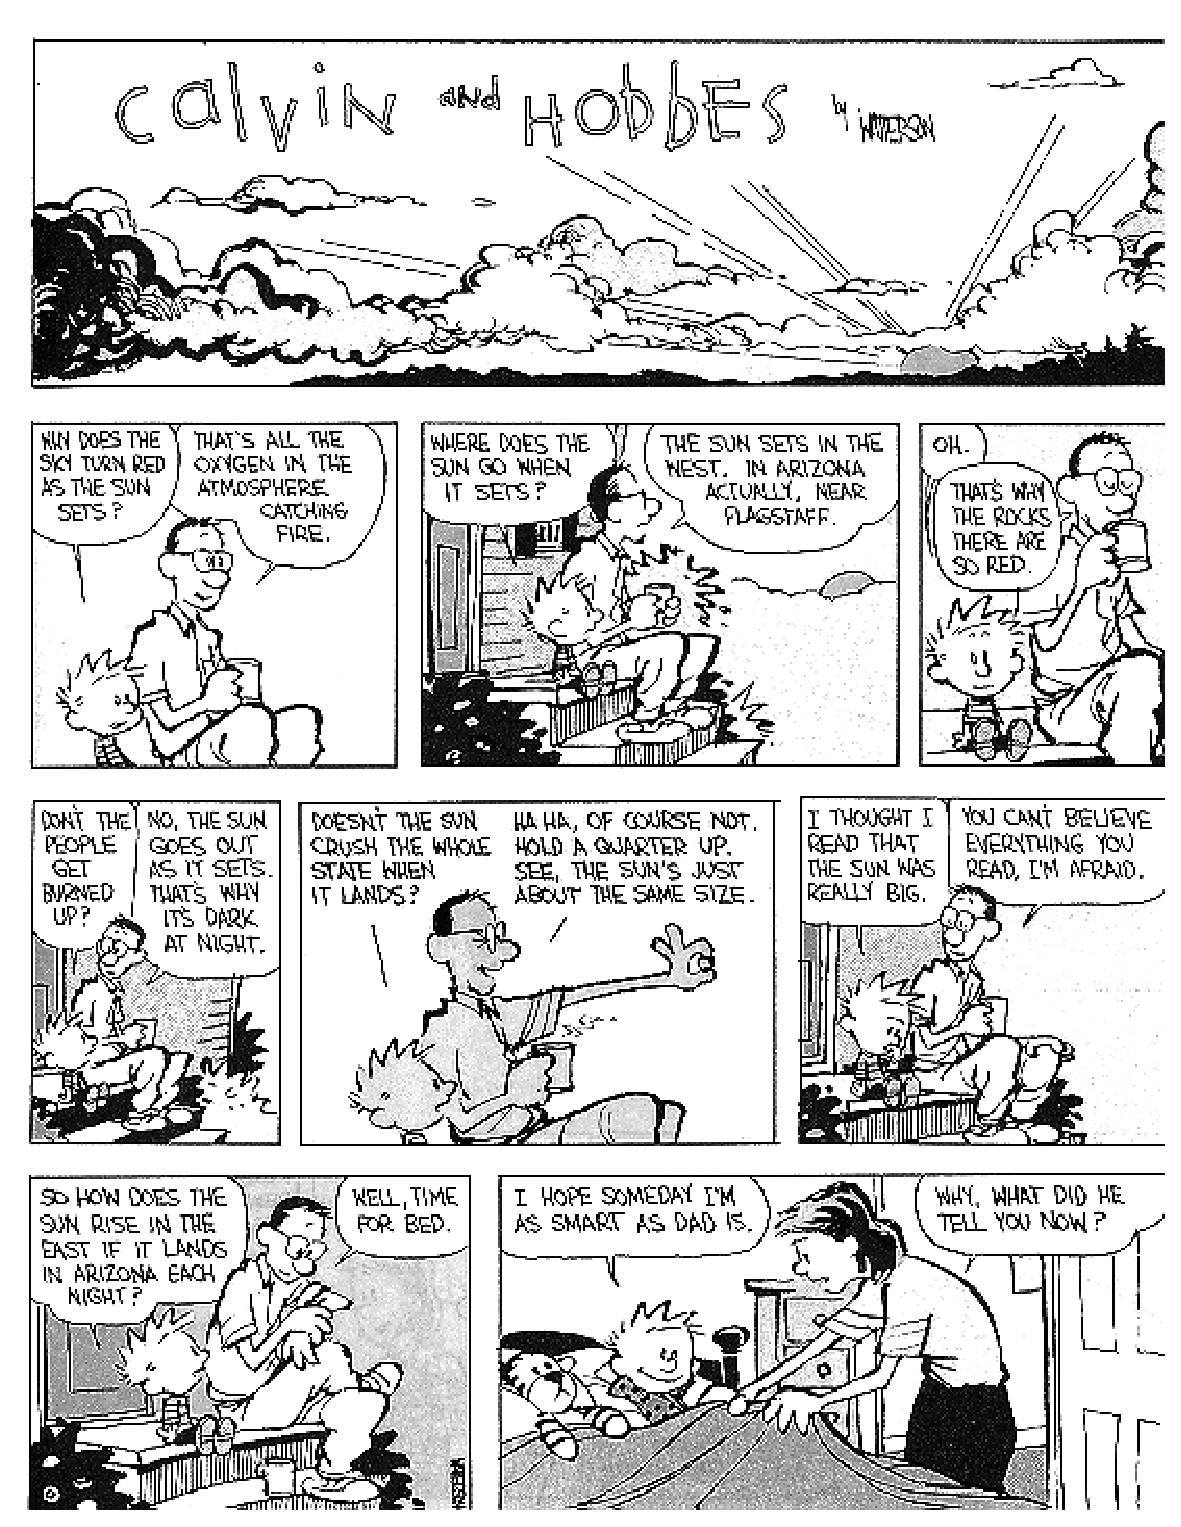
\includegraphics[width=3in]{localdistance/calvin-sun.eps}\par}
\centerline{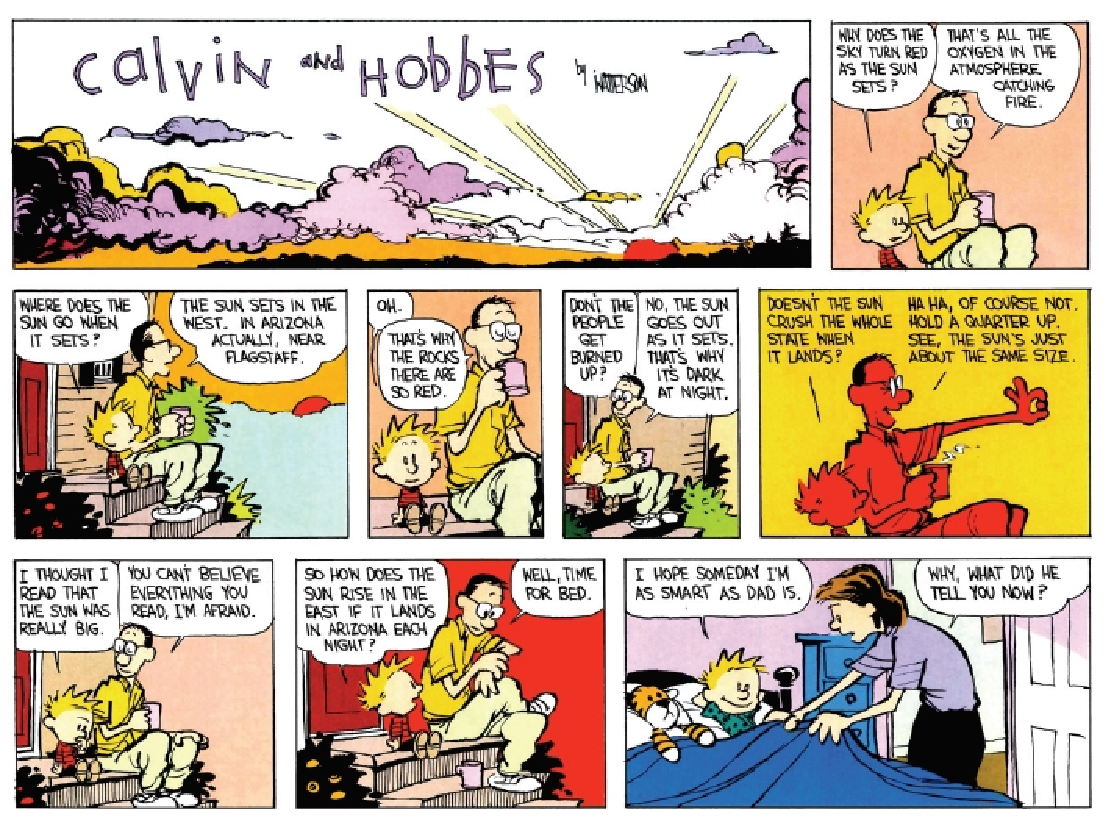
\includegraphics[width=\textwidth]{localdistance/calvin-sun-color.pdf}}
\answerspace{0.5in}

One of the most important things to know about an astronomical
object is its distance from us.  Unfortunately, measuring distances
is often very hard.  There's no one method that works for
finding the distances to all astronomical objects, so 
astronomers have come up with a number of different
methods that work in different circumstances.

One method is based on the familiar observation that a 
faraway object looks smaller than an identical nearby object.
One way to gauge the distance to an object, then, it to measure
its apparent size.  The smaller the apparent size, the greater
the distance.

\pagebreak[4]

For instance, suppose you wanted to know the distance to a faraway
galaxy.  Also, suppose that there's a much closer object of the
same apparent size (like the Sun and the quarter Calvin's Dad is holding).
If the two objects have the same apparent size, then the nearby one
can just block the view of the faraway one, like this:

%\centerline{\epsfxsize 6in\epsfbox{localdistance/localdistance1.eps}}
\centerline{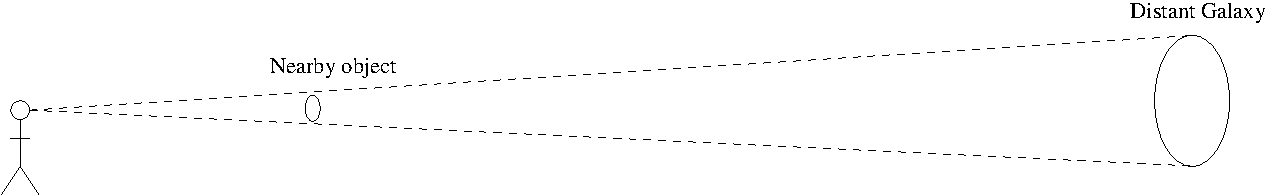
\includegraphics[width=6in]{localdistance/localdistance1.pdf}}

Let's give some names to the sizes and distances in this picture:
\begin{itemize}
\item $s_1$ is the size (diameter) of the nearby object.
\item $d_1$ is the distance from the observer to the nearby object.
\item $s_2$ is the size (diameter) of the distant galaxy.
\item $d_2$ is the distance from the observer to the distant galaxy.
\end{itemize}

Indicate these four distances on the diagram above.  Then write down 
an equation giving the mathematical relationship between these
quantities.  (Hints: You might want to think in terms of 
proportions and ratios.  You might possibly want to think back to 
what you learned about similar triangles in geometry class all those years ago.
If you're stuck on this --- or anything else --- ask me.)

\vskip 1in

If we can somehow manage to determine the size and distance of
the nearby object, and the size of the faraway galaxy, we can 
use this relationship to find the galaxy's distance.

To see how this works in practice, you're going to use this
technique to measure the distance to a nearby building on campus.

\begin{enumerate}

\item You have a sheet of transparent plastic with lines of different
thicknesses marked on them.  Take the sheet outside and find a place
where you have a clear view of one of the windows of a nearby 
building (Gray Court and the Modlin Center are the best choices).  Bring
a length of string and a meter stick with you.

\item One partner should hold up the plastic sheet with the lines
oriented horizontally and adjust the sheet so that one of the lines just
blocks the window in the distant
building (that is, so that the apparent thickness
of the line is the same as the apparent height of the window).
The other partner should measure the distance from the person's eye to
the line.  (I suggest you stretch the string between the eye and
the plastic sheet, then measure the length of the string.)
Write down those values here.  Also, write down the thickness of the
line that you used.

{\bf Note:} Whenever you write down a measurement,
you must also write down its units.

\answerspace{1in}

\pagebreak[2]
\item To determine the distance to the other building, you'll need one more bit
of information: the actual size of the window.  We're going to make
an assumption (which may not be correct) that the windows in the other
building
are the same size as the windows in our classroom.  Go back
to the classroom, measure the height of the window, and record it here.

\answerspace{1in}

\item Using the relationship between $s_1,d_1,s_2,d_2$, together
with the values you just recorded, determine the distance
from here to the other building:

\answerspace{1in}

To see how well you did, determine the distance using
the aerial photograph from Google maps that I'll hand out. Here's how.

\item The scale bar at the lower left of the photograph
shows the distance on the page that corresponds to 50 meters of
actual distance. Measure the length of this bar, and use the result
to determine how many meters of actual distance correspond to 1 cm
on the page.

\answerspace{1in}

\item Mark on the page your approximate location when you made the
measurement and the location of the window. Measure the distance between
the two points on the page in centimeters.

\answerspace{1in}

\pagebreak[3]
\item Use this information to determine the distance from your
observation point to the other building in meters.

\answerspace{1in}

\end{enumerate}

Are your two determinations of the distance significantly
different?  If so, what do you think the main reasons are?  Which
measurements might have been inaccurate?  What assumptions might
have been incorrect?

\answerspace{2in}

%\newpage
%
%\begin{center}
%{\bf Lab: Apparent Size and Distance}\\
%{\bf Summary of Key Results}
%\end{center}
%
%\vfil
%
%{\bf NAMES:}
%
%\vfil
%
%Distance from eye to sheet:
%\vfil
%
%Thickness of line on sheet:
%\vfil
%
%Height of window in lab:
%\vfil
%
%Distance to building determined from the above numbers:
%\vfil
%
%Scale of photograph: how many meters corresponds to 1 cm on page?
%\vfil
%
%Distance to building as measured on page:
%\vfil
%
%Distance to building as determined from the above numbers:
%\vfil
%\eject
%
%
%

\chapter{Angular Measurements}


In astronomy, we often talk about the ``angular size'' of an object.
This is just a way of expressing how big the object appears to be, or
in other words how much of our field of view it takes up.  For
instance, in the picture below (which is the same as the picture in
your previous lab), the two objects have the same angular size,
because they ``fill up'' the same angle in the observer's
field of view.

\medskip
\centerline{\epsfxsize 6in\epsfbox{figs/localdistance1.eps}}
\medskip

The angular size is related to the actual size of the object and the
object's distance.  That relationship is going to be extremely useful
to us, so I want you to spend a little while right now working it out.

Here's a picture of an object.  The angular size is the angle $\alpha$
on the left.  The distance from the observer to the object is $d$, and
the actual size of the object is $s$.  Our goal is to relate the
three numbers $\alpha,s,d$.

\medskip
\centerline{\epsfbox{figs/angularsizefig1.eps}}
\medskip

(Note: Your textbook uses the symbol $D$ instead of $s$ for
the size of the object.  I don't like that, because I think it's
too easy to mix up $d$ and $D$, so I'm going to call it $s$ instead.)

We can use trigonometry to relate these three numbers, but the
mathematics is a bit annoying.  Fortunately, as long as the angle
$\alpha$ is very small (which it almost always is
in astronomical observations), there is a simplified
relationship between these numbers that doesn't involve
any trig.  Here's how it works.

In the picture below, the straight line on the right
represents the
object.  The length of this line is the exact value of $s$, the object's
size.  The picture also shows a curved line.  That curve is an arc
of a circle centered on the observer.  Because it's curved and not straight,
the length of this arc is not quite the same as $s$.  On the other hand,
if the angle $\alpha$ is very small, then this curve is almost the same
length as the straight line.  For this reason, {\it we are going to allow
ourselves to pretend that the length of that curved arc is the
same as $s$.}  To figure out the length of the straight line, we'd
need trig, but we can figure out the length of the arc with just
geometry.


\medskip
{\epsfbox{figs/angularsizefig2.eps}}
\medskip

Here's yet another picture of the situation.  Now the observer is at
the center.  The solid arc represents the size of the object being observed,
and $d$ is the distance from observer to object.  The dashed circle
is an imaginary circle centered on the observer.

\medskip
\centerline{\epsfxsize 2.5in\epsfbox{figs/angularsizefig3.eps}}
\medskip

Well, let's get started.



1. Suppose that the angle $\alpha$ is one degree.  What fraction
of the whole circle is covered by the arc $s$?

\vskip 1in

2. Remember that the circumference of a circle is $2\pi$ times the
radius.  What is the length of the arc $s$, in terms of the distance
$d$?  Continue to assume that $\alpha$ is one degree.
(Your answer here should say $s=$ something times $d$.)


\vskip 1in


Repeat steps 1 and 2, but this time assume that $\alpha=2^\circ$.


\vskip 1.5in

Repeat steps 1 and 2, but this time don't assume any particular
value for $\alpha$.  Instead, your answers will be algebraic
expressions including $\alpha$ as an unknown variable.
Your final result should say $s=$ something involving both $\alpha$ and $d$.


\vskip 2in

Once you've got this expression worked out, show it to me.  This
extremely useful fact is known as the ``small-angle formula.''

Now that you know the small-angle formula, what do you use it for?
The main thing is that any time you know two of the numbers $\alpha,s,d$,
you can use the formula to get the third one.  Try these out:

The Moon is 3476 kilometers in diameter, and it's 380\,000 kilometers
away.  What is the angular size of the Moon?

\vskip 1in

The Sun's angular size is 0.53 degrees, and the Sun is 150 million
kilometers away.  What's the Sun's diameter in kilometers?

\vskip 1in

Most of the time, angles in astronomy are much smaller even than one degree.
For this reason, astronomers usually measure angles in units called
{\it arc-minutes} and {\it arc-seconds}.  One arc-minute is one-sixtieth
of a degree:
$$
1' = \left({1\over 60}\right)^\circ.
$$
($'$ means ``minute''; $^\circ$ means ``degree.'')
One arc-second is one-sixtieth of a minute:
$$
1''=\left({1\over 60}\right)'.
$$
($''$ means ``second.'')

How many arc-seconds are in one degree?

\vskip 1in

A decent astronomical telescope can see things whose angular size is
as small as $1''$.  How far away would your lab partner have to be in
order for the angular distance between their eyes to be equal to
$1''$?  You'll have to measure the distance between your partner's
eyes to answer this.  (If your partner is any further away than this,
then the telescope would no longer be able to see your partner's eyes
as two separate objects; they'd be blurred into one blob.)


\vskip 1in

Optional question:
If you know and remember your trig and feel like it, try answering
the last question using trig instead of the small-angle formula.  Does
it make a significant difference in the final result?


\chapter{Resolution of the Human Eye}

Everyone knows that there are limits to how well we can see. Some
objects are too small or too close together for our eyes to distinguish
them. The same goes for any telescope or other observing device we
might use: even the Hubble Space Telescope has limits to the level of fine
detail it can ``see.''
We define the \textit{resolution} of an observing device (an eye
or a  telescope,
for instance) to be the \textit{angular size} of
the smallest details it can see. The smaller the resolution, the
better the device is at seeing fine details.
In this lab, you will measure the resolution of your own eyes.

You will be given a piece of paper that has a pair of black dots on it,
along with a single oval-shaped blob that's about the same size as the
pair of dots. If you look at the paper from a short distance, it's
easy to tell the pair of dots apart from the single blob, but from
a great distance you can't tell which is which.
We say that you can \textit{resolve} the pair of dots if you
can tell that the two dots really are two dots, not one.

\paragraph{Measurements.}
Take the sheet with the dots on it and move quite far away (10 meters
or so) from your lab partner. Hold the sheet up either right-side up
or upside-down, but don't tell your partner which. From this
distance, your partner should not be able to tell the difference
between the pair of dots and the single blob.
Your partner
should then walk slowly toward you until he or she can tell which 
one is pair of dots. Measure the distance between the two of you
at the moment your partner can first tell with confidence
which is which.

Repeat this procedure at least three times. Switch the orientation
of the paper randomly, so that your partner doesn't know the ``right''
answer. Switch roles, so that each partner is the ``observer'' 
at least three times.
List the individual measurements below, and
also compute the average distance for each partner.

\vfil\eject
%\line{\ }

%\vskip 2.5in

The resolution of your eyes is the angular separation between the
two dots when you can just barely tell that there are two of them.
To figure out this number, you need to know the 
separation between the two dots (to be precise, the separation between
their centers). Measure this separation.

\vskip 1in

Use the above information to calculate the resolution of each
partner's eyes. Give your answer in degrees and also in
arc-minutes. Remember that one arc-minute ($1'$) is $1\over 60$ of
a degree.

\vskip 2.5in

Once you've got your answers, record them on the whiteboard,
so that everyone can see the range of resolutions.

Now suppose that you repeated the experiment using dots that
were twice as big, and twice as far apart.
What would you expect the distance between partners to come out to be?

\vskip 1in

What would you expect the resolution to come out to be?

\vskip 1in

The back of the page contains dots that are twice as large.
Try the experiment and see. (You don't need to do 3 repetitions per partner
this time; just one is fine.) Are the results consistent with
your predictions?

\vskip 1in

\paragraph{Questions.}

Here are some questions to test whether you know what you're doing
with all this stuff. Some of these questions have to
do with resolution, and some are other applications of
the small-angle formula.
You don't have to turn these in, but 
you just might have a quiz some time soon that asks questions very similar
to these.

Note that I've obnoxiously used a variety of different units here.
If you need to look up unit conversions, go ahead. 
In some cases, I may have deliberately left out a number you need, in which case
you should estimate it as best you can.

(In case you're wondering, on a quiz or exam, I will not expect you to know 
numbers such as the number of meters
in a light-year or the distance from Earth to Sun.
You should know the basic
metric-system prefixes, like the number of centimeters in a meter
or meters in a kilometer.)

\begin{enumerate}

\item The Moon is 384\,000 kilometers away. There are two large
craters on its surface, which you can just barely distinguish from
each other with the naked eye. How far apart are the craters?

\item At the Battle of Bunker Hill, the rebels were supposedly
told, ``Don't shoot until you see the whites of their eyes.''
How close would the British be at this point?

\item You're standing on a deserted road, late at night. A vehicle
is approaching you. At first, you can't tell whether it is a car (with
two headlights) or a motorcycle (with one). How close will the vehicle
be before you can tell? 

\item The resolution of the Hubble Space Telescope is about $0.1''$ (that's
0.1 arc-seconds). How many times better than your eye is this?

\item The two dwarf planets Pluto and Charon (formerly known as the planet
Pluto and its moon) are about 20\,000 kilometers
apart. They are about 29 astronomical units from the Earth. What is
the resolution of a telescope that can just barely resolve these two
bodies? Give your answer in arc-seconds.

\item Suppose that another star somewhere nearby has a planet
orbiting it at exactly the same distance as the Earth is from the Sun.
How close would the star have to be in order for the Hubble
Space Telescope to be able to see the planet and star as separate
objects? Give your answer in light-years.\footnote{Actually,
seeing other planets is even harder than this question suggests.
Looking for something very faint right next to something
very bright is extremely difficult.}
The closest star is 4.2 light-years
away. Is this close enough?

\item One of the stars in the handle of the Big Dipper is actually
a pair of stars called Alcor and Mizar. The two stars have
an angular separation of about $12'$ and are about 1 light-year
away from us. How far are the two stars from each other?
Give your answer in meters and in astronomical units.

\item The supergiant star Betelgeuse has an angular diameter of $0.044''$
 and is 427 light-years from Earth. What is Betelgeuse's
diameter? If the Sun suddenly swelled up until it was as big as Betelgeuse,
which of the planets of the solar system would it engulf?


\item A typical distance between neighboring galaxies is 2 million
light-years. A good ground-based telescope has a resolution of about $2''$.
How far away must a galaxy be if an observer using this telescope
has difficulty resolving it (that is, telling it apart from its
neighbors)? Because the Universe is not infinitely old, there's
a maximum distance we can see of about 50 billion light-years (light
from greater distances hasn't had time to reach us). Bearing this
in mind, is there ever a problem telling galaxies apart from their
neighbors with a telescope like this?

\item 
\begin{quote}
``Riders!'' cried Aragorn, springing to his feet. 
``Many riders on swift steeds are coming towards us!''

``Yes,'' said Legolas, ``there are one hundred and five. 
Yellow is their hair, and bright are their spears. Their leader is very tall.''

Aragorn smiled. ``Keen are the eyes of the Elves,'' he said.

``Nay! The riders are little more than five leagues distant,'' said Legolas.

{\hfill J.R.R. Tolkien, \textit{The Two Towers}}
\end{quote}

Roughly what is the resolution of Legolas's eyes? 


\end{enumerate}

%\newpage

\paragraph{Answers.} 

For purposes of the answers below, I'll assume that the resolution
you found for your eye was $2'$ (two arc-minutes). 

\begin{enumerate}

\item 220 km.
\item I'll estimate that the white of your eye is about 1 centimeter
across (from the edge of your iris to the edge of your eye). Something
about that size can be resolved at a distance of about 20 meters.
\item $2'$ is $120''$, which is 1200 times bigger than $0.1''$, so 
the Hubble space telescope has a resolution about 1200 times better than
your eye.
\item Assuming the headlights are about 2 meters apart, the distance
comes out to about 3.4 kilometers.
\item About $0.95''$.
\item 33 light-years. So the nearest star is close enough.
\item $3.3\times 10^{13}$ m, or 220 AU.
\item The diameter is $8.6\times 10^{11}$ m or 5.7 AU. All
planets within half this distance, or about 2.85 AU, 
of the Sun would be engulfed. That's Mercury, Venus, Earth, and Mars. 
(Jupiter's orbit is about 5 AU in radius.)
\item About $2\times 10^{11}$ light-years. This is about 200 billion
light-years, which is much bigger than the maximum distance
we can see, so telling galaxies apart from their neighbors
isn't generally a problem even for very distant galaxies.
\item We've got to make some estimates here. Let's say that
Legolas can resolve features that are as small as 0.1 meters. (If
his resolution were much worse than this, then I don't think he could
tell a tall person from a short person. Naturally, if you used
a somewhat different number, that's fine.) 
Five leagues is about 15 miles, or about 25 km.
The resolution corresponding to these numbers is $0.0002^\circ$, or $0.85''$.
Legolas does about as well as a good astronomical telescope.

\end{enumerate}

\setcounter{chapter}{3}
\setcounter{page}{14}
\chapter{Daily Motion of Stars}
% (Stellarium version)}

This lab has a few purposes:
\begin{itemize}
\item To get used to some features of the {\it Stellarium}
program.
\item To identify some prominent constellations and asterisms
that can be seen from our location.
\item To see how stars move in the night sky.
\end{itemize}

\bigskip

{\bf A. Messing around.}

Start up {\it Stellarium}, and spend a few minutes playing around with
some of its features. Appendix \ref{app:stell} lists a bunch of things
you can do. Here are some specific things you should try. Refer
to the Appendix for details about how do do these things.

\begin{enumerate}
\item Adjust the time and date. When you first start the 
program, it will show the sky at the current time.  It's much
more interesting to see the sky at night. You can
also examine what things look like at different times of year.

\item Speed up the flow of time by a large amount, so that
a day goes by in just a few seconds.

\item Initially, the program is showing you the view of the sky
from here in Richmond. Switch to some other locations.

\item Click on a star or other astronomical object.
Information about that body should appear on the screen.
Some of that information may not make sense yet, but it will!

\item Drag the image around (hold down the left mouse button
and move the mouse around) to look at different parts 
of the sky.

\item Zoom in to look at a small patch of the sky, then
zoom back out
(using the mouse wheel or the page-up/page-down keys).
Note the display at the bottom that says ``FOV.'' This stands
for ``field of view,'' and it indicates the size of the patch of sky
that's visible on the screen at that moment. Watch how the FOV changes
as you zoom in and out.

\item Click on the ``find'' icon and search for various celestial
objects. 
Try Uranus, for example, or Polaris (which
is the name of the North Star).


\item The pop-up menus in the lower left
contain a bunch of buttons you can click to change
the appearance in various ways. I've listed the ones I think
are most useful in the Appendix. Try these out. Some are harder
to understand than others.

\end{enumerate}

\bigskip

{\bf B. Big Dipper, Mizar, and Alcor.}

Once you're done messing around, set your location back to Richmond,
looking north, with a nice, large field of view (say $90^\circ$ or so).
Set the
time to 10:00 tonight.

You should see the Big Dipper in the northeast.
Turn
on the constellation labels and lines.  Notice that the Big
Dipper is not a full constellation; it's just part of the larger constellation
Ursa Major (the Great Bear).  A group of stars like the Big
Dipper, which is easily
identifiable and has a name, but which isn't a whole constellation,
is called an ``asterism.''  

The second star in the handle of the Big Dipper is called Mizar.
Click on this star to select it, and move it into the center
of the field of view. 
Then zoom in on this star until you can see
another star called Alcor right near it.  Find the angular separation
between these two stars.
What is the angular separation?

\vskip 1in

This separation is visible to the naked eye, if you have good eyesight.
Next time you're out on a clear night, look to see if you can spot both
Alcor and Mizar.

Zoom in on Mizar still further, and you'll eventually see that it
splits into two stars. Amazingly enough, although \textit{Stellarium}
might not tell you this, each of those two stars is itself a double
star system.
Unfortunately, these two pairs are too close together for us to 
see them separately, even with our best telescopes.  (How do we know
that they're there, then?  Good question! We'll answer it eventually.) 
In fact, in 2009 it was discovered that Alcor is actually a double
star system as well.
So when you look at Mizar you're really seeing four stars,
and if you look at both Alcor and Mizar, you're seeing six stars.

What is the angular separation between Mizar and its companion (not
Alcor -- the closer one)?

\vskip 1in

Select Mizar by clicking on it (if it's not still selected). 
You'll see some information about it in the upper left corner,
including the distance to the star in light-years. 
Use the small-angle formula to determine the separation between
Mizar and its companion.  The small-angle formula will give you
an answer in light-years.  Convert this to meters and to astronomical
units.


\vskip 2in

 
Zoom back out to the largest field of view, look toward the north again.

\bigskip

{\bf C. Other Constellations.}

Identifying constellations isn't a big part of this course (after
all, there's no science involved in constellation-spotting).  Still, it's
good to know where a few prominent constellations are.

The two stars at the end of the bowl of the Big Dipper (Merak and Dubhe)
are called the pointer stars.  Draw an imaginary line from Merak to Dubhe,
and extend it about six times the separation between those stars.
You'll hit the star Polaris, which is the tail end of the
Little Dipper (the constellation Ursa Minor).  Polaris is also known
as the North Star.  Polaris isn't a terribly bright star -- in fact,
none of the stars in Ursa Minor are very bright -- but it's still
important.  It's the one star in the sky that all the others seem
to rotate around.  (More on this later.)

Look to the West from Polaris to find the constellation Cassiopeia.  It
looks like a W (on its side at the moment).  The stars in Cassiopeia
are quite bright, and Cassiopeia is easy to spot in the night sky pretty
much all the time.  Cassiopeia and the Big Dipper are probably the most
useful constellations to use when orienting yourself to the night sky.

In the winter, the other easy constellation to spot is Orion. Find
it in the southern sky.

That's enough with constellations for now; we'll do more when we actually
do some observing.

\bigskip

{\bf D. Daily Motion of Stars.}

Make sure you're looking North, with a large field
of view (at least $90^\circ$).  Turn off the effects of Earth's 
atmosphere.
This will make it so that the sky is dark during the day, so that
you can see the stars all the time.  (Astronomers would love
it if this were possible in real life!)

Set time to go at much faster than the normal rate,
so that a day takes only a a few seconds.
Observe how the stars move.
The stars move in circles, with the star Polaris at the center.
Note that some of the stars move in circles that always stay
above the horizon, while others rise and set below the horizon.
Stars that never set below the horizon are called ``circumpolar.''

Of course, whether a star sets below the horizon or not depends on
the exact shape of the horizon. To keep things simple, let's assume that
we're looking at the stars from a location with a nice, flat horizon
(no hills or trees to get in the way). Here's one way to make this happen
in \textit{Stellarium}: click on ``Sky and viewing options'', then
the ``Landscape'' tab, then check the ``Ocean'' box. As you'll
see, that shows you what things would look like if you were surrounded
by a nice, flat ocean.

How many of the seven main stars in the
Big Dipper are circumpolar? (Here I'm counting all of
Alcor and Mizar as one star.)


\vskip 1in

Now change locations to Boston, Massachusetts.  How many of the stars
in the Big Dipper are circumpolar when viewed from Boston?

\vskip 1in

When Santa looks at the stars from the north pole, how do they
appear to move?  What percentage of the stars he sees are circumpolar?
Make a prediction first, then try it.

\vskip 1in

Now switch your location to Santiago, Chile.  Find the center of the
circles that stars appear to move in from this location (hint: look South).
What constellation is this in? (There are several constellations right near
this point. Astronomers have defined precise boundaries between the
constellations. To see which one this point is in, figure out how to turn
on the ``constellation boundaries'' in \textit{Stellarium}.)

\vskip 1in

Note that there is no bright star right at the center of these circles:
Polaris is the North Star, but there is no South Star.

Go back home to Richmond.
Pick a star that's not circumpolar (that is, one that rises and sets).
Record the time that this star rises on one day, and the time it
rises on the next day.  Make sure your times are accurate to the minute.
How much time elapses between successive risings of the star?

\vskip 1in

Repeat for a few other stars.  Is the result always the same?

\vskip 1in


The length of time between successive risings of a star is called a
``sidereal day.''  How different is a sidereal day from  an ordinary
day?


%\chapter{Daily Motion of Stars}

This lab has a few purposes:
\begin{itemize}
\item To get used to some features of the {\it Sky Safari}
app.
\item To identify some prominent constellations and asterisms
that can be seen from our location.
\item To see how stars move in the night sky.
\end{itemize}

\bigskip

{\bf A. Messing around.}

Start up {\it Sky Safari}, and spend a few minutes playing around with
some of its features. Appendix A lists a bunch of things
you can do. Here are some specific things you should try. Refer
to the Appendix for details about how do do these things.

\begin{enumerate}
\item Adjust the time and date. When you first start the 
program, it will show the sky at the current time.  It's much
more interesting to see the sky at night. You can
also examine what things look like at different times of year.

\item Speed up the flow of time by a large amount, so that
a day goes by in just a few seconds.

\item Initially, the program is showing you the view of the sky
from here in Richmond. Switch to some other locations.

\item Tap a star or other astronomical object, and then hit ``Info.''
Information about that body should appear on the screen.
Some of that information may not make sense yet, but it will!

\item Drag the image around 
to look at different parts 
of the sky.

\item Zoom in to look at a small patch of the sky, then
zoom back out
Note the display at upper right that lists two numbers in 
degrees (something like $124.4^\circ \times 95.4^\circ$).
That indicates the 
``field of view,'' which is the size of the patch of sky
that's visible on the screen at that moment. Watch how the field of
view changes as you zoom in and out.

\item Tap the ``search'' icon and search for various celestial
objects. 
Try Mars, for example, or Polaris (which
is the name of the North Star).


\item The ``Settings'' button at the bottom will take you to a
bunch of options that you can use to change the appearance in
various ways.
I've listed the ones I think
are most useful in the Appendix. Try these out. Some are harder
to understand than others.

\end{enumerate}

\bigskip

{\bf B. Big Dipper, Mizar, and Alcor.}

Once you're done messing around, set your location back to Richmond,
looking north, with a nice, large field of view (say $90^\circ$ or so).
Set the
time to 10:00 tonight.

You should see the Big Dipper in the northeast.
Turn
on the constellation labels and lines (if they're not already on).  
Notice that the Big
Dipper is not a full constellation; it's just part of the larger constellation
Ursa Major (the Great Bear).  A group of stars like the Big
Dipper, which is easily
identifiable and has a name, but which isn't a whole constellation,
is called an ``asterism.''  

The second star in the handle of the Big Dipper is called Mizar.
Select this star and move it into the center
of the field of view. 
Then zoom in on this star until you can see
another star called Alcor right near it.  Find the angular separation
between these two stars. (As always, see the Appendix for details.)

What is the angular separation?

\vskip 1in

This separation is visible to the naked eye, if you have good eyesight.
Next time you're out on a clear night, look to see if you can spot both
Alcor and Mizar.

Zoom in on Mizar still further, and you'll eventually see that it
splits into two stars. Amazingly enough, 
each of those two stars is itself a double
star system (You can find this in the detailed Object Info for
Mizar, if you don't believe me).
Unfortunately, these two pairs are too close together for us to 
see them separately, even with our best telescopes.  (How do we know
that they're there, then?  Good question! We'll answer it eventually.) 
In fact, in 2009 it was discovered that Alcor is actually a double
star system as well.
So when you look at Mizar you're really seeing four stars,
and if you look at both Alcor and Mizar, you're seeing six stars.

\vskip 1in

Bring up the information screen for Mizar, and 
find the distance to the star in light-years. The
angular separation between the two stars that make up Mizar is about
$14''$ (for some reason, \textit{Sky Safari} gave me a different
number, but this is the right one).
Use the small-angle formula to determine the separation between
Mizar and its companion.  The small-angle formula will give you
an answer in light-years.  Convert this to meters and to astronomical
units.


\vskip 2in
Zoom back out to the a nice, large field of view, say $60^\circ$ or more
across, and
look toward the north again.

\bigskip

{\bf C. Other Constellations.}

Identifying constellations isn't a big part of this course (after
all, there's no physics involved in constellation-spotting).  Still, it's
good to know where a few prominent constellations are.

The two stars at the end of the bowl of the Big Dipper (Merak and Dubhe)
are called the pointer stars.  Draw an imaginary line from Merak to Dubhe,
and extend it about six times the separation between those stars.
You'll hit the star Polaris, which is the tail end of the
Little Dipper (the constellation Ursa Minor).  Polaris is also known
as the North Star.  Polaris isn't a terribly bright star -- in fact,
none of the stars in Ursa Minor are very bright -- but it's still
important.  It's the one star in the sky that all the others seem
to rotate around.  (More on this later.)

Look to the West from Polaris to find the constellation Cassiopeia.  It
looks like a W (on its side at the moment).  The stars in Cassiopeia
are quite bright, and Cassiopeia is easy to spot in the night sky pretty
much all the time.  Cassiopeia and the Big Dipper are probably the most
useful constellations to use when orienting yourself to the night sky.

In the winter, the other easy constellation to spot is Orion. Find
it in the southern sky.

That's enough with constellations for now; we'll do more when we actually
do some observing.

\bigskip

{\bf D. Daily Motion of Stars.}

Make sure you're looking North, with a large field
of view (at least $90^\circ$).  Turn off the effects of Earth's 
atmosphere.
This will make it so that the sky is dark during the day, so that
you can see the stars all the time.  (Astronomers would love
it if this were possible in real life!)

Set time to go at much faster than the normal rate,
so that a day takes only a a few seconds.
Observe how the stars move.
The stars move in circles, with the star Polaris at the center.
Note that some of the stars move in circles that always stay
above the horizon, while others rise and set below the horizon.
Stars that never set below the horizon are called ``circumpolar.''

Of course, whether a star stays above the horizon or not depends on
the detailed shape of the horizon. To keep things simple, let's assume
we're looking from a location with a nice, flat horizon (no
hills or trees to block our view). To set this up, go to
``Settings,'' and then to ``Horizon \& Sky,'' and choose to display
the horizon as an ``Opaque area.''
With  this setup, how many of the seven main stars in the
Big Dipper are circumpolar? (Here I'm counting all of
Alcor and Mizar as one star.)

\vskip 1in

Now change locations to Boston, Massachusetts.  How many of the stars
in the Big Dipper are circumpolar when viewed from Boston?

\vskip 1in

When Santa looks at the stars from the North pole, how do they
appear to move?  What percentage of the stars he sees are circumpolar?
Make a prediction first, then try it. (The North pole isn't one
of the listed locations in \textit{Sky Safari}, but you can go there
by typing in its latitude, which is $90^\circ$ north.)

\vskip 1in

Now switch your location to Santiago, Chile.  Find the center of the
circles that stars appear to move in from this location (hint: look South).
What constellation is this in?

\vskip 1in

Note that there is no bright star right at the center of these circles:
Polaris is the North Star, but there is no South Star.

Go back home to Richmond.
Pick a star that's not circumpolar (that is, one that rises and sets).
Record the time that this star rises on one day, and the time it
rises on the next day.  Make sure your times are accurate to the minute.
How much time elapses between successive risings of the star?

\vskip 1in

Repeat for a few other stars.  Is the result always the same?

\vskip 1in


The length of time between successive risings of a star is called a
``sidereal day.''  How different is a sidereal day from  an ordinary
day?


%% Solar cell makes a circuit with a 100-ohm resistor. Measure voltage
%% across resistor. Power is proportional to voltage. (Not voltage squared --
%% we must be current-limited.)
%%
%% Use PASCO Basic Optics light source. Round stand with angles
%% marked on it at the other end of the short PASCO optical bench.
%% Same setup should work tolerably well for inverse square law, or 
%% are we better off using the other light sensors there?


\section{Intensity of Solar Radiation}

\makelabheader

\bigskip
There are two main reasons winter is colder than summer:
\begin{itemize}
\item The Sun is up for fewer hours per day in the winter.
\item The Sun is lower in the sky in winter.  This means
that sunlight strikes Earth's surface at a shallow
angle, which lowers the intensity
of the radiation striking the Earth's surface.
\end{itemize}

In this lab, you'll verify these statements. In particular,
you'll find out the amount of time the Sun is up at different
times of the year,
you'll see how high the Sun rises in the sky in summer and winter,
and you'll check that radiation striking a surface at
a shallow angle deposits less energy than radiation that is
closer to perpendicular.

\bigskip

{\bf A. Amounts of sunlight at different times of the year.} 

Start up \textit{Stellarium}, and set the date to June 21, the 
first day of summer. Determine the times of sunrise and sunset on that
day, by running time forward and backward and watching the position of the Sun.
(Use a flat horizon.)
How many hours of daylight are there on that day?

\answerspace{1in}

Repeat this procedure on December 21, the first day of winter.

\answerspace{1in}

What is the ratio of these two values? That is, how many times
greater is the amount of sunlight on June 21 compared to December 21?

\answerspace{1in}

\pagebreak[2]
{\bf B. Angle made by the Sun in summer and winter.}

\medskip


Set the time to noon on June 21 (the first day of summer).
Make \textit{Stellarium} draw the \textit{meridian}, which is a line 
in the sky going from due north, directly overhead, to due south.
On any given day,
the moment the Sun crosses the meridian is the moment when it's
highest in the sky.  
At what time does the Sun cross the
meridian on this date?

\answerspace{1in}

Why doesn't the Sun cross the meridian at exactly noon?  (There
are several reasons.)

\answerspace{1.5in}

Select the Sun and view the information on it. Find the
Sun's \textit{altitude}.
This is the angle indicating the Sun's height above
the horizon. (90$^\circ$ would be directly overhead,
and 0$^\circ$ would be right on the horizon.)  What is the Sun's
maximum altitude on this date?

\answerspace{1in}

Repeat this procedure to find the Sun's maximum altitude on 
December 21, the first day of winter.

\answerspace{1in}



{\bf C. Effect of angle on the amount of solar radiation.}

\medskip

Next, you'll check to see how much of an effect this difference in angles
makes to the amount of radiation striking the Earth.  The light
bulb on your table will represent the Sun.  You will use a solar
cell to represent a small piece of the Earth's surface.
Your goal is to see how the
amount of radiation from the bulb changes as the
angle of the cell is varied. In particular, how much more radiation strikes
the cell when the light is beating down on it from almost directly above
(like sunlight in summer),
compared to the amount when the light strikes it at a shallower angle
(like sunlight in winter)?

Place the bulb at one end of the optical bench, and place
the round platform with angle markings at the other end.
We'll call the center of the round platform
the ``observer's location,'' and we'll call the bulb the ``Sun.''

Start the program called 
``solarcell.cap'' on the lab computer.  
This program allows the computer to display the amount of radiation striking
the solar cell.

Place the solar cell at the observer's location,
facing directly towards the Sun. The surface of the cell
should be perpendicular to a line going from the cell to the Sun.
In the picture below, the cell should be oriented along the
line marked ``Perpendicular.''

\centerline{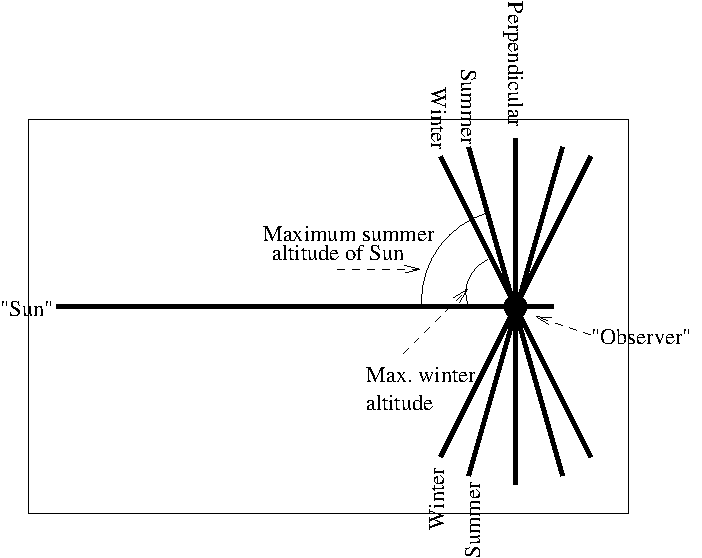
\includegraphics{solarcell/solarcellfig.pdf}}

Turn on the light bulb, and hit the ``Record''
button 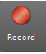
\includegraphics[width=0.2in]{solarcell/capstone-record.pdf} on the
computer screen.  You should see a graph showing the amount
of radiation striking the solar cell as time passes.  Try placing
your hand in front of the solar cell to block the light.  The
reading should go down.

Let the computer record data for about 20-30 seconds.  
We want to know the average amount of light striking the solar
cell. To find this out, you need to select a range of
data where the graph looks reasonably flat.
Hit the button that looks like this, near the top of your screen:
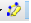
\includegraphics[width=0.2in]{solarcell/capstone-select.pdf}.
That'll create a rectangle that you can move to select the
region of data you want to use.
Once you've highlighted a stretch of data, the computer should
display the average (``Mean'') of those numbers.  This is the 
average amount of radiation striking the solar cell during
this time period.  Record this value:

\answerspace{0.25in}

This represents the amount of power that strikes the solar cell
if it were lying flat on the ground, and the Sun was beating down
on it from directly overhead. In fact, though, the Sun is never
directly overhead (at least, not from a location like Richmond).
The highest the Sun ever gets in the sky is the altitude you found
for the first day of summer in part B.

Rotate the solar cell so that it the angle it makes with
the line to the Sun corresponds to the altitude of the
Sun on that date. (This means orienting the cell so that it
lies along one of the lines marked ``Summer'' in the picture above.)

\answerspace{1in}

\pagebreak[2]
Repeat the procedure with the solar cell aligned on the other ``summer''
line.  

\answerspace{1in}

The last two values should be close to the same.  Average them
together:

\answerspace{1in}

Repeat this procedure with the two winter lines to end
up with an average amount of radiation striking the cell
when it's at the winter angle:

\answerspace{2in}

You should have found that the amount of radiation is greatest
when the cell is perpendicular, a bit less when it's at the summer
angle, and much less when it's at the winter angle.

How many times more intense is the midday solar radiation in summer
than in winter?

\answerspace{1in}

Let me repeat the main point. Part A and this part 
show two different reasons why it's hotter in summer: there are more
hours of daylight in summer, and the sunlight is more intense.




\setcounter{chapter}{5}
\setcounter{page}{22}
\chapter{Celestial Navigation}
% (Stellarium version)}

In the old days, before GPS, sailors figured out where they were
by looking at the positions of the stars. In this lab, you'll
see how that worked. To be specific, you'll look at the question
of how to use the positions of celestial 
objects to determine your latitude and longitude.

Our reason for doing this is not that I expect you to find yourself
lost at sea without access to GPS (although anything's possible,
I guess). It's because
figuring out how celestial navigation works is a good way to make
sure you understand how things move in the night sky.

\section*{Latitude}

As it turns out, determining your latitude (i.e., how far north or
south of the equator you are) is much easier than determining your longitude.
The easiest way is to observe the location of the star Polaris.
As you know, Polaris is very close to the North Celestial Pole, or in
other words almost directly above the Earth's North Pole. For
purposes of the questions below, you can assume that Polaris is
exactly at the North Celestial Pole.

Suppose you were standing at the Earth's North Pole, which is at a latitude
of $90^\circ$ north. In which direction would you have to look
in order to see Polaris?

\vskip 1in

Now suppose you measured the \textit{altitude} of Polaris. 
As we've seen, the 
altitude of an object is the angle that describes how far above
the horizon that object is located. To be specific, draw an imaginary
line from you to Polaris, and draw an imaginary horizontal line (pointing
toward the horizon) directly below Polaris. The altitude means
the angle between those two lines.

If you were at the north pole, what would the altitude of Polaris be?

\vskip 1in

Now suppose you were at the equator (which is at a latitude
of $0^\circ$). In which direction would you have to look in order to see
Polaris?

\vskip 1in

What would the altitude of Polaris be?

\vskip 1in

Based on the above considerations, you can guess that there might
be a \textit{very} simple rule relating the altitue of Polaris
to the observer's latitude. What do you think that relationship is?

\vskip 1in

We could test this observation using actual observations of Polaris at
night, but instead let's test it with \textit{Stellarium}. 

Start up \textit{Stellarium}. 
Find the star Polaris and select it. Look at the information in
the upper left, and find the star's altitude. What is the altitude of
Polaris?

\vskip 1in

What is our latitude here in Richmond? (You can find this out by looking
at ``Location'' in \textit{Stellarium}, or I'm sure Google knows it.)
\vskip 1in

Do the two values you just found agree, at least roughly, with your
expectations? (If the degrees agree but there's a discrepancy in the
arc-minutes, that's close enough.)

\vskip 1in

If you're ever lost at sea, you now know how to find your latitude,
by observing how high Polaris is in the sky.

\section*{Longitude}

Suppose you wake up one night and find yourself in a boat tossing about
in the middle of the ocean. Using the method above, you figure out
your latitude. Now how are you going to find your longitude? As we'll see,
this
turns out to be a much harder problem than finding latitude.

Suppose your
latitude comes out to be $20^\circ$ north. 
To keep things (relatively) simple, let's suppose that there
are just two possibilities
for longitude: either you're at a longitude of $25^\circ$ west,
or you're at a longitude of $55^\circ$ west. 

Set the time in \textit{Stellarium} to about 10:00 tonight,
and set your location to be a latitude of $20^\circ$ north and
a longitude of $25^\circ$ west. (You can type these numbers
directly into the Location box. Just enter the
number of degrees, and leave out the minutes and
seconds.) Orient your view so that you're looking north,
with the horizon at the bottom and a pretty large 
field of view (about $60^\circ$ or so). Note a couple of
landmarks to orient yourself in the sky. You should be able
to see the Big Dipper (upside-down) and the bright star Capella, for
instance.

Once you've got this set, take a screen shot by hitting control-S.
Check that the screen shot was saved. (I think
it end up in your Pictures folder.)
Open it up and take a look at it to make sure it looks
the way you expect. 
Once you see that the file looks right, go back to \textit{Stellarium}.

Now change your location to $55^\circ$ west longitude (keeping
the latitude and the time the same).
Take a screen shot of the sky from this new location.

Now advance the time by two hours, from 10:00 pm to midnight.
Take one more screen shot.

At this point, you should have three screen shots.
\begin{enumerate}
\item Longitude: $25^\circ$. Time: 10:00 pm.
\item Longitude: $55^\circ$. Time: 10:00 pm.
\item Longitude: $55^\circ$. Time: midnight.
\end{enumerate}
Incidentally, I should mention that the times in \textit{Stellarium}
are always times in our actual location (Richmond). That is, 10:00 pm
means 10:00 pm Eastern time, regardless of the observer's location.

Two of these three images should look almost identical, and one
should look significantly different. Which one is not like the others?

\vskip 1in

\newpage

Now, let's get back to your plight as you sit bobbing in your boat
in the middle of the ocean. Suppose that you have a timekeeping
device (wristwatch cell phone, etc.) that is set to Eastern
time. Using this, along with your observation of the night
sky, can you tell which longitude you're at? If so, explain
briefly how. If not, explain briefly why not.

\vskip 3in

Suppose that you \textit{don't} have an accurate timekeeping device
on board the boat. Can you tell what longitude you're at by
observing the sky? If so, explain
briefly how. If not, explain briefly why not.

\vskip 3in

In the 18th century, the British government offered large
cash prizes for anyone who could figure out an accurate way
to determine the longitude of a ship at sea. 
In 1765, John Harrison was awarded a \pounds 10\,000 prize
for solving this problem. (It's hard to
figure out precise equivalents, but this is 
equivalent to  millions of dollars today.) 
What do you think Harrison invented?

\vskip 1in

Back to you on your boat. Suppose that you had a clock with you
on your boat, but it wasn't very accurate. Suppose that you use the clock
to determine your longitude, but unbeknownst to you the clock is off by
two hours. (For instance, you think it's midnight, when really it's 10:00
pm.) By how many degrees will your longitude determination be off?

\vskip 1in

Suppose that your clock were only off by one minute instead. How far
off will your longitude determination be?

\vskip 1in

One degree of longitude corresponds to an actual distance of about 50 
kilometers. If your clock were off by one minute of time, 
how far off would your determination of your location be (in kilometers)?

\vskip 1in

If you were a ship's captain 
trying to avoid hitting undersea rocks
and shoals, this level of inaccuracy would be a real problem.


\section{The Moon}

\makelabheader

\bigskip

In this lab, you'll check a bunch 
of things about the motion and phases of the Moon.
%Although most of the things in this lab can be done in \textit{Sky
%Safari}, there are one or two things that can't, so we'll 
%use the more powerful \textit{Stellarium} on the lab PCs.



%% \medskip

%% {\bf A. Getting familiar with Stellarium}

%% Since we haven't ued \textit{Stellarium} yet in class, 
%% spend a few minutes playing around with it to learn how it works.
%% Pretty much everything you've done so far in \textit{Sky Safari} can
%% also be done in \textit{Stellarium}. In particular, try out the following.
%% Consult Appendix B for details about how to do these things.

%% \begin{enumerate}
%% \item Adjust the time and date. When you first start the 
%% program, it will show the sky at the current time.  It's much
%% more interesting to see the sky at night. You can
%% also examine what things look like at different times of year.

%% \item Speed up the flow of time by a large amount, so that
%% a day goes by in just a few seconds.

%% \item Initially, the program is showing you the view of the sky
%% from here in Richmond. Switch to some other locations.

%% \item Click on a star or other astronomical object.
%% Information about that body should appear on the screen.
%% Some of that information may not make sense yet, but it will!

%% \item Drag the image around  to look at different parts 
%% of the sky.

%% \item Zoom in to look at a small patch of the sky, then
%% zoom back out
%% (using the mouse wheel or the page-up/page-down keys).
%% Note the display at the bottom that says ``FOV.'' This indicates
%% the field of view, which as you know 
%% indicates the size of the patch of sky
%% that's visible on the screen at that moment. 

%% \item Click on the ``find'' icon and search for various celestial
%% objects. 
%% Try Mars, for example, or Polaris.


%% \item The pop-up menus in the lower left
%% contain a bunch of buttons you can click to change
%% the appearance in various ways. I've listed the ones I think
%% are most useful in the Appendix. Try these out. Some are harder
%% to understand than others.

%% \end{enumerate}


\bigskip

{\bf A. Sidereal and Synodic Months}

A {\it sidereal month} is the length of time it takes the
Moon to make one complete motion around the sky with respect to the
stars.  In other words, at the end of a sidereal month, the Moon
appears in the sky next to the same stars as it did at the beginning
of the month.
A {\it synodic month} is the time it takes the Moon to go through one
full cycle of phases (from full Moon to full Moon, for example).
You'll use {\it Stellarium} to measure the length of both sidereal and
synodic months.

Start up {\it Stellarium}.  Make the ground transparent and turn
off the Earth's atmosphere, so that we can see what the Moon
is doing at all times. This makes our lives much easier
than the real-life observers who first figured all this stuff out:
they could only see the Moon when it was above the horizon at night.
Again, consult the Appendix to see how to do these things, and of course
ask me if you can't figure it out.

First, step forward in time until the Sun and Moon are right
next to each other in the sky. This is the next time when
the phase of the Moon will be new.
Determine, to within an accuracy of about an hour or so, the
moment when the Moon and Sun are closest to each other in
the sky.
Record the date and time:

\answerspace{1in}

Now let time run forward for a bit less than a month, until the phase of the Moon is nearly new
again.  Just as before, find the moment, accurate to the nearest hour,
when the Moon and Sun are closest together.  Record the date and time:

\answerspace{1in}

Based on these results, what is the length of a synodic month?
Give your answer as a decimal number of days, with at least
one digit after the decimal point.

\answerspace{1in}

\pagebreak[1]
Now you'll figure out the length of a sidereal month.  Click on a star
that's very near the Moon, and keep the field of view centered
on that star. Record the date and time
when that star passes closest to the Moon, accurate to the
nearest hour.  

\answerspace{1in}

Then let the time advance
for a bit less than a month, until you see the marked star pass close to the Moon
again.  Record the time it passes closest to the Moon, accurate
to the nearest hour.

\answerspace{1in}

Find the length of a sidereal month as a decimal number of days.

\answerspace{1in}

The year is 365.24 days long.  How many synodic months are there 
in a year? (Give your answer as a decimal number with at least one
digit after the decimal place).

\answerspace{1in}

How many sidereal months are there in a year?

\answerspace{1in}

You should find that the difference between these two numbers is
very close to 1.  (If you don't find this, let me know.)  This
is a general rule relating sidereal and synodic periods for
all satellites.  You might enjoy trying to figure out why
it's true.  (Then again, you might not.)

\bigskip

\pagebreak[1]

{\bf B. Phases of the Earth}

\medskip

{\bf Question:} 
Suppose the Moon is in a waxing crescent phase as seen from the
Earth.  An astronaut on the Moon looks at the Earth.  What
phase of the Earth does she see?

I want you to figure out the answer to this question on your
own first, and then test it with {\it Stellarium}.

Draw a diagram showing Earth, Sun, and Moon when the Moon is
a waxing crescent.  Indicate the directions of the Earth's orbit
around the Sun and the Moon's orbit around the Earth.

\answerspace{2in}

Based on this diagram, what is the answer to the question above?
(Your answer should be something like ``full Earth,'' ``waning
crescent Earth,'' ``waxing gibbous Earth.'')

\answerspace{1in}

Now test your answer.  Adjust the time until the phase of the Moon
is waxing crescent.  Then click on the Location icon, and
change the location to the Moon.
Adjust the view until you see the 
Earth.  Does its appearance agree with your prediction?  (For
instance, if you predicted the Earth would be in a crescent phase, is it?)
Allow time to run forward.  Is the Earth waxing or waning?
Does this agree with your prediction?


\chapter{Apparent Motion of the Planets}

The motion of the stars in the night sky is pretty simple: they
go in circles about the north celestial pole, making one complete
circuit per sidereal day. The motion of the Sun and Moon are a bit
more complicated: they share in the daily motion of the stars, but
they gradually drift from west to east relative to them. In other words,
as the stars race around the north celestial pole, the Sun
and the Moon gradually fall behind.

The motion of the planets has a lot in common with the Sun and Moon,
but it's a bit more complicated. One of the most important scientific
advances in all of human history was Copernicus's correct
explanation of why the planets seem to move the way they do. 
To understand what Copernicus figured out, we first have
to examine how the planets appear to move in the sky.

\paragraph{Jupiter's daily motion.}
The first thing to realize is that, on any particular day, the
planets seem to move in pretty much the same way as the stars: they
circulate about the north celestial pole, rising in the east and setting
in the west, taking about one day to go all the way around. Let's start
by making sure of this.

%% Start up \textit{Sky Safari}.\footnote{If you prefer, you 
%% can do everything in this lab using \textit{Stellarium.} The main thing
%% to remember there is that the ``equatorial and horizon coordinate systems''
%% in \textit{Sky Safari} correspond to the ``equatorial and azimuthal
%% mount'' in \textit{Stellarium}.}
Start up \textit{Stellarium}.
Locate the planet Jupiter. If it's not up above the horizon during the night
time, shift time forward a month at a time until it is. Once you've
reached a time when Jupiter is up at night,
let
time run rapidly for several days, 
and observe Jupiter's motion. You
should find that, if you don't look too closely anyway, it moves in
pretty much the same way as the stars it's next to.

Determine, to an accuracy of about a minute or so, the time when Jupiter sets
on two successive days. How much time elapsed between these two occurrences?

\vskip 1.5in

If you did the same thing with a star (i.e., measured the difference between
two times  the star set), what would you find? You can try it if you want,
but I hope you know what the answer is.

\vskip 1in

The two answers should be very similar. Depending on how carefully you 
measured, you may or may not have found a small difference between them.
Now let's examine that small difference more carefully.

\paragraph{Jupiter's slow drift with respect to the stars.}
Over the course of a few days, Jupiter (and the other planets) seem to
move in approximately the same ways as the stars, but there are 
small differences, which build up to become quite important
over longer periods of time. To examine those differences,
it helps to ``turn off'' the daily motion of everything.
To do this, switch to the ``equatorial mount.''
You should also turn off the effects of daylight,
so that you can watch the planets at all times.


Set the time to the present, locate Jupiter, and center it in the field
of view. Set time running forward \textit{very} rapidly, so that a year goes by
every few seconds. You should see Jupiter generally drift from right
to left with respect to the stars, but sometimes reverse itself
and drift from left to right.\footnote{If you're keeping Jupiter 
centered in the field of view, of course, it won't actually move at all.
When I say you'll see Jupiter go from right to left
with respect to the stars, what I really mean
is that you'll see the stars slip past it from left to right.}
When we look at the sky in the equatorial (stationary-sky) point of view, 
east is always on
our left and west is on our right, so we say that Jupiter
usually goes from west to east, but sometimes reverses direction and
goes from east to west.

The times when Jupiter goes ``backwards'' (east to west) are called
periods of \textit{retrograde motion}. The next thing we want to 
do is look for patterns in when Jupiter goes into retrograde motion.

Set the time back to the present, and start it running forward
rapidly. Find the beginning and end of the next three time periods
when Jupiter is in retrograde motion. It's hard to spot the
exact moment when retrograde begins or ends. You don't
have to get the exact date right -- just determine the month and
year. To get you started, I'll tell you that Jupiter will
next go into retrograde motion in about April 2019.


While you're at it, find all the times 
when Jupiter will be
in \textit{conjunction} with the Sun during this period (from
now through the end of the third retrograde period). 
This means the time when
it passes right next to the Sun in the sky.

List your results (three time periods when Jupiter is in retrograde
and all the moments when it's in conjunction) below.

\vskip 3in

On a blank sheet of paper, make a time line covering the entire
range of all these times, and the periods of retrograde and conjunction.

Summarize your results in a sentence or two.

\vskip 1in

\paragraph{Motion of other planets.}
Try the same thing with the planets Mars and Venus.
To be specific, identify the next three times when the planet is 
in retrograde, and all the times of conjunction from now until the end of those
three
retrograde periods. Make a time line for each.

\vskip 5in

Which of these two planets shows a pattern very similar to Jupiter?
Which is different?

\vskip 1in

Make a guess about why one of these planets is not like the others.

\vskip 1in




\section{Sidereal and Synodic Periods}

\makelabheader

\medskip

\paragraph{Part 1. An example.}
Imagine two runners, Ellen and Peter,
running around a circular track, starting out
next to each other. Each runner runs at a constant speed, but one 
is faster than the other: Ellen takes 8 minutes to go around the track
once, and Peter takes 10 minutes. Let's call these two times
$E$ and $P$ respectively: $E=8$ minutes and $P=10$ minutes.


Eventually, Ellen will ``lap'' Peter -- that is, she will have gone around
the track one time more than him, so that she's right
next to him again. I want
you to figure out how much time it takes for this to happen.
There are different ways to do this, but one thing that might help
is to figure out where Ellen and Peter are after 10 minutes have gone by.
By how much (what fraction of a lap) will Ellen will be ahead of 
Peter? How many times would you have to repeat this until Ellen
had lapped Peter?

Your final answer should be a number of minutes. This is the amount
of time it takes for the two runners to go from a particular configuration
(right next to each other) to the same configuration again. If Peter and Ellen
were planets, this would be called the ``synodic period'' of the two planets.

\answerspace{2in}


We're going to want a general relationship giving the synodic period
in terms of the ``sidereal periods'' $P$ and $E$. It turns
out that the relationship is simplest if we express it in terms
of the reciprocals of these numbers.

What are the reciprocals of the three numbers $P$, $E$, $S$ for
this situation? (Express them as decimals, not fractions.)
$$
\frac{1}{P}=
\hspace{1.7in}
\frac{1}{E}=
\hspace{1.7in}
\frac{1}{S}=
\hspace{ 1.7in}
$$

Can you spot a relatively simple mathematical relationship
between these three numbers? Write it down in the form of an equation
involving $\frac{1}{P}$, $\frac{1}{E}$, $\frac{1}{S}$.


\answerspace{2in}


\paragraph{Part 2. The general rule.}
The rule you wrote down in the previous part turns out to apply
no matter what $P$ and $E$ are. We're going to check that this
is true algebraically now. In this section, you should forget 
the specific numerical values for $P,E,S$ (that is, the 10 minutes, 8 minutes,
etc.). We're going to work out an expression that is true
for different possible values of these quantities.

As before, $E$ stands for the time that Ellen takes to go around
the track once, and $P$ stands for the time that Peter takes. $S$
stands for the ``synodic period'' -- that is, the time it takes for
Ellen to pull ahead of Peter by one full lap.

After a time $S$ has gone by, how many laps has Ellen run? Your
answer will be an algebraic expression involving $E$ and $S$.\footnote{If
you don't know what to do, try thinking it through with a particular
number in mind. For instance, suppose that it takes Ellen 2 minutes
to run a lap (so $E=2$ minutes), and suppose $S=20$ minutes. How
many laps will Ellen have run in those 20 minutes? 
Write down whatever you did to get your answer, but use the letters
$S$ and $E$ in place of 20 and 2, and you have the expression I want.}

\answerspace{1.5in}

After a time $S$ has gone by, how many laps has Peter run?
Your answer will be an expression involving $S$ and $P$. 

\answerspace{1.5in}

\pagebreak[4]

By definition, $S$ is the time at which Ellen has run one more
lap than Peter. That means that your answers to the two previous
questions must differ by one. Write down that last sentence in
the form of an algebraic equation.

\answerspace{1in}

Do some algebraic manipulations on that equation until
it looks like the equation you wrote down at the end of Part 1.



\vfil

You're done! You've just derived the general rule relating sidereal
and synodic periods. When we apply this in astronomy, $E$ will
be the sidereal period of the Earth (one year), $P$ will be the sidereal
period of another planet (the length of a year on that planet), and 
$S$ will be the synodic period.

A couple of quick notes:
\begin{itemize}[nosep]
\item In this derivation, we assumed that Ellen was faster than Peter.
That means that the formula we derived only works if the other
planet has a longer period than the Earth. That turns out to be true
for all of the planets further out than the Sun (Mars, Jupiter, etc.).
The planets Mercury and Venus, go faster than the Earth, so the
final formula looks slightly different. You could work it out by the
same sort of reasoning if you wanted to, or you can look it up in
your textbook.
\item In this expression, we usually give all of the periods in years, but
you don't have to. You can use any unit of time you want, but it has
to be the same unit for all three quantities.
\item The main reason this relationship is useful is in determining
sidereal periods for other planets. After all, we know $E$ (one year),
and $S$ is easy to measure -- just observe the time it takes between
two successive times the planet goes into opposition. So the
most common use of this rule is to find the one remaining quantity,
namely $P$.
\end{itemize}





\section{Kepler's Third Law}

\makelabheader

\answerspace{1in}

Kepler's third law says that the period of a planet's orbit
(the time to orbit once, called $P$) and the radius
of its orbit (called $a$) are related like this:
$$
P^2=ka^3.
$$
Here $k$ is a constant.  Its numerical value depends on what units
we choose for $P$ and $a$, but it's the same for all of the planets.

Jupiter and its moons look like a mini-solar system: the moons orbit
Jupiter in pretty much the same way that the planets orbit the Sun.
So it's natural to wonder whether Jupiter's moons obey Kepler's third
law.  In this lab, you'll use 
{\it Stellarium} to simulate
observations of the moons to test Kepler's third law.

Start up \textit{Stellarium}. Turn off the effects of Earth's
atmosphere/daylight, and make the Earth transparent, so that we can see
Jupiter all the time. (Once again, we're making our lives a bit easier than
it is for real astronomers: in reality, we could only make
the sort observations in this lab at certain times of the year.)
Set the program to the equatorial (stationary-sky) mount.
Find Jupiter, center it in the field
of view, and set the field of view to a size where you can clearly 
see Jupiter and its four Galilean moons (Io, Europa, Callisto, Ganymede).

Let time run forward at a pretty high speed and observe the orbits of 
the moons.  The orbits are really very close to circular, but we're
viewing them from the side, so the moons appear to move back and forth.

Pick one of the moons, and run time forwards and backwards until the
moon is at its greatest separation from Jupiter.  (Be as accurate as
possible; you can probably determine the time to within about 10 minutes
for the fastest-moving moon and less than an hour for the slowest one.)
Measure the angular separation between Jupiter and the moon at this moment.
Repeat the procedure for all four moons.  Record your results in the table
on the last page.  You'll initially get the angular separation
in arc-minutes and arc-seconds.  Convert your answer to a number of 
arc-seconds.  For instance, if you got a value of $2'$ and $20''$, you
would record $140''$ (because $1'$ is $60''$, and $2\times 60+20=140$)..

How far is Jupiter from us at the time these observations are being taken?
Record the distance in A.U. here:

\answerspace{1in}

Use the small-angle formula to convert the angular separations
for all four moons into actual separations.  These will be the
maximum distances the four moons get from Jupiter; in other words,
they'll be the radii of the moons' orbits.  Record them in the data table,
along with their units. (Be sure to keep at least a couple of significant
figures for these numbers.)

Now that you know the radii of the orbits, the next step is to find the
periods.  The most accurate way to do this is to measure the time between
moments when the moon passes in front of or behind Jupiter.

Set the date back to today, and then advance time
forwards or backwards until one of the moons is just
passing in front of the edge of Jupiter from the left.  (Aim for
an accuracy of about 5 minutes.)  Record
the date and time, and also the ``Modified Julian Date (MJD).''
See Appendix \label{app:stellarium} for details on how to do this.

Let time advance until that moon
is just passing in front of the left edge of Jupiter again (one complete
orbit later).  Record the date, time, and MJD again.  

Next, you should determine the time that elapsed
between these two measurements.  This is the period of the moon's orbit.
Give the result as a decimal number of days. (You can do this by working
out the difference between the two dates and times, but it's much easier
using the MJDs. In fact, that's what MJDs are for!)

Repeat this procedure for all four moons. Each time you start working on a
new Moon, set the time back to the present day.

Now that you know the period and the radius of all four moons,
you can test Kepler's third law.  Square all of the periods to get $P^2$,
and cube all the radii to get $a^3$.  Take the ratio $P^2/a^3$.
Kepler's third law says that this should be the same for all four
moons.  Is it?

\answerspace{1in}

A couple of follow-up questions:

1. Is the numerical value of $k$ for Jupiter's moons the same
as the value for the planets orbiting the Sun?  To answer this,
figure out the value of $k$ for the Earth's orbit around the
Sun using the same units as you used for Jupiter's moons.

\answerspace{2.2in}

2. Why did we have to use the moons of Jupiter for this lab,
instead of using Earth's Moon?



\begin{center}
\begin{tabular}{|l|l|l|l|l|}
\noalign{\hrule}
{\bf MOON} & Io & Callisto & Ganymede & Europa \\
\noalign{\hrule}
Max. angular separation & \qquad\qquad\qquad\qquad & \qquad\qquad\qquad\qquad &
\qquad\qquad\qquad\qquad &\qquad\qquad\qquad\qquad \huge\strut\\
from Jupiter ($'$ and $''$) & & & &\huge\strut \\
\noalign{\hrule}
Max. angular separation & & & & \huge\strut\\
from Jupiter ($''$) & & & & \huge\strut\\
\noalign{\hrule}
Radius of orbit & & & & \huge\strut\\
& & & & \huge\strut\\
\noalign{\hrule}
Date/time of first & & & & \huge\strut\\
crossing of Jupiter &  & & & \huge\strut\\
\noalign{\hrule}
MJD of first crossing  & & & & \huge\strut\\
& & & & \huge\strut\\
\noalign{\hrule}
Time of second & & & & \huge\strut\\
crossing of Jupiter &  & & & \huge\strut\\
\noalign{\hrule}
MJD of second crossing  & & & & \huge\strut\\
& & & & \huge\strut\\
\noalign{\hrule}
Orbital period & & & & \huge\strut\\
& & & & \huge\strut\\
\noalign{\hrule}
$P^2$ & & & & \huge\strut\\
& & & & \huge\strut\\
\noalign{\hrule}
$a^3$ & & & & \huge\strut\\
& & & & \huge\strut\\
\noalign{\hrule}
$k$ & & & & \huge\strut\\
& & & & \huge\strut\\
\noalign{\hrule}
\end{tabular}
\end{center}


\documentclass[twoside]{report}
\renewcommand{\chaptername}{Lab}
\usepackage{graphicx}
\usepackage{epsf}
\textwidth 6in
\textheight 9in
\topmargin -0.2in
\oddsidemargin 0.3in
\evensidemargin -0.3in
\parindent 0pt
\parskip 6pt





\begin{document}
\chapter*{Lab 6$1\over 2$ \\ Phases of Venus}


One of the most important things Galileo observed with his telescope is that
Venus has phases like the Moon.   This was the ``smoking gun'' that showed
that the earth-centered (pre-Copernicus) system couldn't possibly be right,
so it went a long way toward convincing people that the Earth really did
go around the Sun.  We're going to examine the phases of Venus to see what
Galileo saw and why it mattered.

Start up {\it Starry Night}, and configure it as follows:  
\begin{itemize}
\item Set the time to noon today.  Set the time step to ``days.''
\item Turn off 
daylight, so that it's possible to see the stars and planets when the
Sun is up.  (Remember that you can do this by clicking on the ``View Options''
tab on the left and unchecking the ``Daylight'' option under ``Local View.'').
\item Turn on labels for the planets by checking the ``Labels'' box next to
``Planets-Moons'' in the ``View Options'' menu.  
\item Set the view to be centered on the Sun (right-click on the Sun and 
choose ``centre'').  
\end{itemize}

Let time run forwards and backwards for a year or two and observe the
motion of Venus.  Note that it swings back and forth past the Sun,
never getting more than a certain angular separation from the Sun in the sky.
Once you've done this, reset the date to today.

Here's one preliminary question before we look at the phases of Venus.  If
you wanted to observe Venus today, at what time of night should you observe?
Specifically, find a rough time when Venus is above the horizon but the Sun
is below the horizon.  The easiest way to do this is to set the time step
to hours and step forward or backward one hour at a time.

Best time to observe Venus these days:

\vskip 0.7in

Note that you've got a fairly narrow window of time when the Sun is
down but Venus is up, so it'd be pretty hard to observe Venus right
now.  The easiest time to observe Venus is when its as far away from
the Sun in the sky as possible.  This is called the time of ``maximum
elongation.''  Set the time back to noon, set the time step to days,
and run time backwards until you find the most recent time of maximum
elongation.  (Hint: it's some time in March 2006.)  Measure the angular
separation between
Venus and the Sun at that time.  (Remember that you can do that by 
dragging the mouse from one object to the other, but be sure the pointer
looks like an arrow, not a hand, when you start.)

Maximum angular separation between Sun and Venus:

\vskip 0.7in

Here's a diagram showing the Earth's and Venus's orbits around the
Sun.  Suppose that the Earth is at the uppermost point in its orbit as
shown, and suppose that Venus is at maximum elongation from the Sun
(so that it appears as far from the Sun as possible in the sky).  Draw
a circle to mark the position of Venus in its orbit.  (There are
actually two possibilities.  One corresponds to the case where Venus
is to the East of the Sun and one to the case where it's to the West.
If you assume everything orbits
counterclockwise, you can figure out which which, although
it's a bit tricky.  For the moment, it doesn't matter which one you choose.)

\begin{figure}[h]
\centerline{\epsfxsize 3in\epsfbox{figs/venus1.eps}}
\end{figure}


Venus, like the Moon, shines by reflected sunlight.  That means that
the only part of Venus we'll see is the part that's illuminated by the 
Sun.  In the diagram above, shade in the half of Venus that's lit up by
the Sun, and then use the diagram to predict the phase of Venus
at this time.  (That is, will Venus appear like a crescent, like
a ``full'' Venus, or what?)

\vskip 0.7in

After you've made your prediction, use {\it Starry Night} to test it.
Center the view on Venus and zoom in to enlarge the image of Venus.
Does it have the phase you predicted?

\vskip 0.7in

Now set the date back to today, and 
zoom in on Venus to observe its phase.  What is the phase of Venus today?

\vskip 0.7in

Based on your observation, is Venus in front of the Sun or behind the Sun
today?

\vskip 0.7in

Zoom back out again, and center the field of view on the Sun.  Let time
run forward until Venus has gone through about half of one orbit.  You
should see it pass by the Sun, go out to maximum elongation, and then come
back until it approaches near the Sun again.  At this point, when
Venus's path is about to cross past the Sun again, is Venus in front
of the Sun or behind the Sun?  (Don't use {\it Starry Night} to answer this; 
use what you know about the orbits.)

\vskip 0.7in

Based on your answer to the previous question, what do you expect the 
phase of Venus to be?

\vskip 0.7in

What do you expect about the angular size of Venus: should it be bigger
or smaller than the last time you looked at it?

\vskip 0.7in

Center the view on Venus and zoom in to test these two predictions.
Did they come out right?

\vskip 0.7in

Keep the field of view centerd on Venus and zoomed all the way in.  Let time
run forward fast for a year or two.  The main things to note are that
Venus goes through a full set of phases (from crescent to full and back),
and that its angular size changes along with its phase.

Earlier, I said that this observation provided strong proof that
the old Earth-centered theory was wrong.  Let's see why.  Remember that
in the old theory the Earth was at the center, the Sun went around the
Earth, and Venus moved on an epicycle between the Earth and the Sun like this:

\begin{figure}[h]
\centerline{\epsfxsize 3in\epsfbox{figs/venus2.eps}}
\end{figure}

At each of the points A,B,C,D in the diagram, what would the phase
of Venus be, according to this model?

A:

B:

C: 

D:

What phases of Venus would {\it never} occur in the earth-centered
model?

\vskip 0.7in

The fact that Venus is observed to have those phases is the ``smoking
gun'' I referred to.

One more thing.  Now that you've measured the maximum elongation of
Venus, you can use it to figure out the radius of Venus's orbit.
Sketch a picture showing Earth, Sun, and Venus at the moment of 
maximum elongation (this will look the same as the diagram on the
second page).  

\vskip 2in

Connect these three bodies with straight lines to form a triangle.
When Venus is at maximum elongation, this triangle will have a right
angle at Venus.  The angle at the Earth is the angular separation
between Venus and Sun (that is, the angle you determined on the second page).
Indicate both of those angles on the diagram.

We also know the length of one side of the triange: the distance from
the Earth to the Sun is 1 AU.  Mark this on your triangle as well.

Now you have a right triangle, and you know one angle (other
than the right angle) and one side.
That means you can use trigonometry to find the lengths of the
other sides.  Determine the radius of Venus's orbit trigonometrically.
(If you don't remember how to do this, ask me.)


\end{document}
\chapter{Finding Masses with Kepler's Third Law}


Newton's version of Kepler's third law goes like this:
$$
P^2=\left[4\pi^2\over G(m_1+m_2)\right]a^3
$$
Here $P$ is the period of an orbiting body, $a$ is the semimajor axis
of the orbit, and $m_1$ and $m_2$ are the masses of the central body
and the orbiting body.  $G$ is a constant whose value is
$$
G=6.67\times 10^{-11}\,{\rm m^3/(kg\,s^2)}.
$$
All the stuff after the $10^{-11}$ is just the units of $G$.
It signifies that we're using seconds for our times, kilograms for
our masses, and meters for our distances.

One incredibly useful thing about this form of Kepler's third law
is that it lets you determine the masses of things.  In fact, most
of the time, if we know the mass of an astronomical object, we figured
it out using this law.

The point of this little ``lab'' is to write this law in a convenient
form for determining masses and then use it to figure out 
masses of some astronomical objects.

The first thing to realize is that usually the mass of the central
body ($m_1$) is much, much larger than the mass of the orbiting
body ($m_2$).  That means that, to an excellent approximation, we can
ignore $m_2$ in Kepler's third law and just write it
$$
P^2={4\pi^2\over Gm_1}a^3.
$$
Since $G$ is a universal constant (always the same known value), 
we can use this to determine the mass of any object, as long as we 
can measure the period and radius of the orbit of something
that's going around that object.

Use this formula to figure out the mass of the Sun in kilograms.  To do this,
consider the orbit of the Earth around the Sun.  What is $P$?
What is $a$?  (Remember that the value of $G$ given above requires
these quantities to be in seconds and meters.)

\vskip 2in

When using Kepler's third law, astronomers usually don't use kilograms,
meters, and seconds.  Instead, they usually measure periods in years,
lengths in A.U., and masses in units of the Sun's mass (``solar masses'').
In these units, the arithmetic becomes a bit simpler.

Consider the Earth's orbit around the Sun again.  In these new units,
what are $P$, $a$, and $m_1$?  (Hint: you don't need your calculator for
this step!)

\vskip 1in

In these units, what is the numerical value of the constant ${4\pi^2\over G}$?
(Plug the values you just wrote down into Kepler's law to see what happens.)

\vskip 1in

Remember that $G$ is a universal constant, as are 4 and $\pi$. 
So the combination ${4\pi^2\over G}$ will always have this simple
numerical value, no matter what orbiting system we're considering (as
long as we're using units of A.U., solar masses, and years).

For instance, let's use Kepler's third law to determine the mass
of the Earth.  Remember that the Moon's orbital period is 27.2 days.
What is this in years?

\vskip 1in

The radius of the Moon's orbit is 384,000 km.  What is this in A.U.?

\vskip 1in

Use these values to determine the Earth's mass in units of solar masses.

\vskip 1.5in

Earlier, you determined how many kilograms there are in a solar mass.
Use this value to convert your answer for Earth's mass into kilograms.

\vskip 1in

The solar system orbits the center of the Milky Way Galaxy in a circular
orbit with a radius of 8.5 kiloparsecs (kpc).  How many meters is this?

\vskip 1in

How many A.U. is it?

\vskip 1in

The solar system's speed in its orbit around the Galaxy is about 220 km/s.
How much time does it take the Sun to make one complete orbit?  (Hint:
how far does it have to travel during one orbit?)  Give your answer in
seconds and in years.

\vskip 2in

Using your values for the period and radius of the solar system's
orbit, determine the mass of the Milky Way Galaxy in solar masses.

\vskip 2in

People have done surveys of all the visible material in the Milky
Way Galaxy (stars, gas, and dust).  They estimate that all the
visible stuff has a combined mass of about $1.0\times 10^{10}$ solar
masses.  What percentage of the total mass of the Galaxy is visible
stuff?  What percentage is stuff we don't see?  (The latter
stuff is called ``dark matter.'')



\chapter{Spectra of Light Sources}

\bigskip\bigskip

In this lab 
you will use a small portable spectroscope to examine several sources
of light.  The spectroscope consists of a slit at one end that lets
light through and a ``grating'' at the other end that splits the light
up into the various colors.  We'll worry a bit later about exactly
how the grating works.

To set up the spectroscope, hold it so that the slit is vertical.  Point
it at a bright light source and look through the other end.  Rotate
the grating end (keeping the slit vertical) until you see horizontal
bands of color on either side of the slit.  These are the colors that
make up the light coming through the slit.

Examine the following light sources with the spectroscope:

\begin{enumerate}

\item The white light coming from the overhead projector.
\item The light from a candle flame.
\item The light from one of the two gas discharge lamps.
\item The light from the other gas discharge lamps.
\item The light from the fluorescent lights in the hallway.
\item The light from the Bunsen burner flame, while someone is placing
a small amount of the white crystalline stuff in it.

\end{enumerate}

Sketch the spectra of all the light sources, then
answer the following questions:.


\begin{enumerate}
\item Which sources have ``continuous'' spectra, meaning that the
light consists of all colors from red to blue?

\vskip 1in

\item For the sources with continuous spectra, can you notice
a difference in the relative amounts of the various colors?
For instance, does one have more red light relative to yellow
or blue, as compared with the other?  (This may be hard to discern,
because the total intensity of the sources is different.)

\vskip 1in

\item Using a chart of spectra that I'll give you, try to determine what gases
are in the two discharge tubes.  Also try to determine
what's in the white powder.

\vskip 1in

\end{enumerate}


\section{The Diffraction Grating}

\makelabheader

\answerspace{1in}

All sorts of waves, including light, do a couple 
of strange things:
\begin{enumerate}
\item Waves bend (a bit) around corners, and spread
out (a bit) when passing through holes. 
This phenomenon is called {\it diffraction}.
\item When two waves meet each other, they
can cancel each other out (if ``peaks'' of the
first wave run into ``valleys'' from the second), 
or they can reinforce each other (if peaks meet up with peaks).
This is called {\it interference}.
\end{enumerate}

A diffraction grating is a device
that takes advantage of both of these phenomena.  They turn
out to be very useful in measuring the wavelength
of light and in splitting light up into its constituent
wavelengths.  

A diffraction grating is just a piece of glass (or something similar)
with many thin parallel lines ruled on it.  When light passes through
the small gaps between these lines, it diffracts.  Light that passed
through the various gaps can then interfere with each other.  In some
directions, the waves that passed through the various gaps cancel each
other out, and in other directions they reinforce each other.  The
result is a pattern of alternating bright and dark patches.

Suppose we take light with wavelength $\lambda$ and
shine it through a diffraction grating.  We then
project the light on a wall and measure the 
positions $x$ of the bright spots (relative to the
center of the diffraction pattern) as shown.  The theory of 
interference tells us that 
\begin{displaymath} n\lambda = {dx\over \sqrt{L^2+x^2}}.  \end{displaymath}
Here $d$ is the separation between lines in the grating and $L$
is the distance from the grating to the wall.  $n$ is called the
``order'' of the spot; it's just an integer: $n=1,2,3,\ldots$.

Note that there are four different quantities in this expression that
have units of length.  One common source of error is to
use incompatible units for these things.  The safest thing is
to use the same units for all four.

One nice thing we can do with all this is measure the wavelength of light.

\bigskip
%\centerline{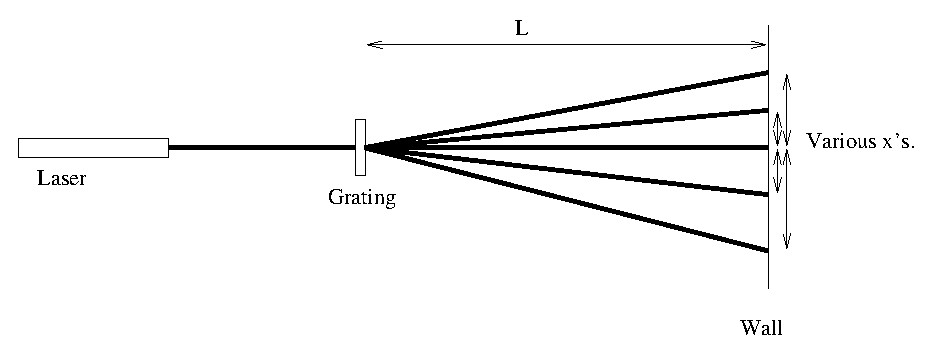
\includegraphics{figs/difffig.eps}}
\bigskip

\begin{enumerate}
\item Record the separation between grating lines: \( d= \)
\item Turn on the laser, being careful to avoid looking directly into the
beam or shining it at anyone. Aim the light beam through the diffraction
grating so that a horizontal series of dots appears on the wall. Adjust
the positions of the laser and grating until you easily see at least
two dots on either side of the brightest (central) dot.
\item Are the dots of the interference/diffraction pattern the same intensity?
Describe the pattern you observe.\answerspace{15mm}

\item Measure the distance from the grating to the wall, $L$,
as well as the distances from the central dot to the first dot to
the right, $x$, and the first dot to the left, $x'$. Compute the average
of these $x$ values and record it as $x_{ave}$. Record all of these
values in the table below.
\item Use the equation above to find the wavelength $\lambda$.
Because these are the first two spots (other than the central dot),
use the value $n=1$.
\item Repeat the procedure using the second dot to the right
of center and the second dot to the left.  This time, use $n=2$ 
when finding the wavelength.
\item If you can see the third pair of dots clearly, repeat the
procedure with $n=3$.
\item Move the laser to a new location (that is, change the
value of $L$) and repeat the procedure for a couple of values
of $n$.  In the end, you should end up with at least
five different determinations of $\lambda$.
\item Compute the average of your determinations of the laser light's
  wavelength and compare it to the expected value, which is printed on the
  laser.
\answerspace{15mm}

\end{enumerate}
\answerspace{0.3cm}
\begin{center}
\begin{tabular}{|c|c|c|c|c|}
\hline 
\( L \) (cm)&
\( x \) (cm)&
\( x' \) (cm)&
\( x_{ave} \) (cm)&
\( \lambda  \) (nm)\\
\hline
\hline 
&
&
&
&
\\
&
&
&
&
\\
\hline 
&
&
&
&
\\
&
&
&
&
\\
\hline 
&
&
&
&
\\
&
&
&
&
\\
\hline 
&
&
&
&
\\
&
&
&
&
\\
\hline 
&
&
&
&
\\
&
&
&
&
\\
\hline
\end{tabular}\answerspace{0.3cm}

\end{center}


Suppose that we shone white light instead of laser light
through the grating.  What would the resulting pattern look
like?

\section{The Spectrum of Hydrogen}

\makelabheader

\answerspace{1in}

In this lab, you will use a spectrometer to measure the wavelengths of 
the spectral lines of hydrogen.  The spectrometer consists of a slit
through which light passes, a diffraction
grating, and a small telescope to focus the light that comes out
of the grating.  The telescope can be rotated in a circle centered
on the diffraction grating.  By measuring the angles at which the
spectral lines appear in the telescope, you can determine the
wavelengths of the lines.

The relationship between the angle and the wavelength is
$$
d\sin\theta = n\lambda.
$$
Here $d$ is the spacing between lines on the diffraction grating, 
and $\theta$ is the angle through which the light from a spectral
line is bent by the grating.
In this spectrometer, we are always seeing the ``first-order'' diffraction
pattern, so $n=1$.
If you don't know or don't remember your trigonometry, don't worry
about it: all you need to know for this lab is how to make your
calculator tell you the sine of an angle.

(Incidentally, this formula is essentially the same as the formula
you used in an earlier diffraction lab, although that one was
written in non-trigonometric form.)

The first thing you'll need to know is $d$, the spacing between
lines on the grating.  The grating should be labeled with a number of
lines per inch or a number of lines per millimeter.  Use this 
to determine the distance between lines in either
meters or centimeters.
(If your
grating is labeled in lines per inch, it may help you to know that one
inch is 2.54 cm.)

\answerspace{2in}

Now that you know $d$, you can determine the wavelength of any spectral
line just by measuring the angle $\theta$ through which the light is bent.

Set up the spectrometer with the hydrogen lamp right against the slit.
Put the grating at the center, so that it is oriented perpendicular to
the direction from the slit.  Look through the telescope, and
gradually move the telescope around until you see the spectral lines
from the lamp.  You don't want the bright spot that you see when the
telescope is lined up pointing straight at the lamp; the spectral
lines you're interested in are visible when it's off to the side.

You should be able to see three spectral lines clearly: one red,
one greenish-blue, and one blue one. I'm going to call the red one
``line 1,'' etc., but note that if you start from the center and
move out from there, you'll see them in reverse order.

For each of the three brightest spectral lines, determine
the wavelength as follows.  

\begin{enumerate}
\item Adjust the spectrometer so that each spectral
line is centered in the telescope, and measure the angle $\theta$
corresponding to each spectral line on both the left and the right.
Note that the angles marked on the spectrometer have $180^\circ$
for light that is not deflected at all.  We'd rather
call that angle $0^\circ$ instead of 180$^\circ$, so you should
subtract $180^\circ$ from your angles.

Measure the angles as accurately as possible.  Note that there is 
a ``Vernier scale'' allowing you to measure an extra decimal place.
I'll explain in class how to read it.

\item For each of the three lines, average the two measurements of
$\theta$ together, and use the resulting value to determine $\lambda$.

\item For each of the spectral lines, record the energy of a photon,
using the rule 
$$
E={hc\over\lambda}.
$$
Planck's constant has the value $h=4.135\times 10^{-15}$ eV s, and
the speed of light is $c=3.00\times 10^8\,{\rm m/s}$.  If you use these
values, and if the wavelength is measured in meters, your energy
will come out in units of electron volts (eV).
\end{enumerate}


\begin{center}
\begin{tabular}{|c|c|c|c|c|c|}\hline
Line        & $\theta_{left}$     & $\theta_{right}$     & $\theta_{average}$ & Wavelength  & Photon Energy \\ 
\hline
& & & & & \\
Line 1 (reddest)  &                             &                              &                    &                    &   \\ \hline
& & & & & \\
Line 2   &                             &                              &                    &                    &   \\ \hline
& & & & & \\
Line 3 (bluest)  &                             &                              &                    &                    &   \\ \hline
\end{tabular}
\end{center}

It turns out that there is a pattern in the energy levels of hydrogen.
The energy levels are of the form
\begin{eqnarray*}
E_1&=&-{A\over 1^2},\\
E_2&=&-{A\over 2^2},\\
E_3&=&-{A\over 3^2},\\
&\ldots&
\end{eqnarray*}
Here $A$ is a constant, whose value you are to determine.

The longest-wavelength visible spectral line of hydrogen
(the red one) occurs when an atom jumps from energy level $n=3$
down to $n=2$.  So the energy of one of those red photons should be
$$
E_3-E_2=-{A\over 3^2}-\left(-{A\over 2^2}\right)=-{A\over 9}+{A\over 4}.
$$
Set this expression equal to the energy you determined for the red spectral
line, and solve for the value of the constant $A$.  Show me the
result when you're done.

\answerspace{2.5in}

Once you know the value of $A$, use it to determine the energy of a photon
emitted when a hydrogen atom jumps from level 4 to level 2:

\answerspace{1in}

From level 5 to level 2:

\answerspace{1in}

These should look similar to the energies you measured for the other
two spectral lines.  If they don't, talk to me.

What is the energy of a photon corresponding to the next spectral line
(a jump from level 6 to level 2)?  What is the wavelength of 
this spectral line?

\answerspace{1.5in}

Using the formula $d\sin\theta=\lambda$, predict the value of $\theta$
at which this spectral line should appear in the spectrometer.
[Note to the trig-averse: to do this, you'll need to use the ``inverse
sine'' (or ``arcsine'' or ``sin$^{-1}$'') function on your calculator.]
Now that you know where to look, see if you can see this spectral line
in the spectrometer.

\answerspace{1in}

One final question: Why do all of these spectral lines correspond
to jumps down to the second energy level?  Why not the first or third,
for instance?



\section{Refraction and Lenses}

\makelabheader 

Over the next few classes, we're going to examine how telescopes work,
but first, we need to figure out some aspects of the behavior of light
when it passes through transparent materials such as glass.

The apparatus for this lab consists of a light source that produces a set
of parallel beams from lasers, along with a variety of transparent and
reflective objects for the light to interact with.  All of these objects
can be attached magnetically to a small whiteboard, so that they can be
easily positioned in various ways.

\paragraph{Part 1: Refraction.}
Plug in the light source and attach it to the whiteboard.  Put
the clear plastic rectangle in front of the source, so that
the light rays hit it at an angle like this:

\answerspace{0.1in}
%\centerline{\epsfxsize 3in\epsfbox{figs/lensfig1.eps}}
\centerline{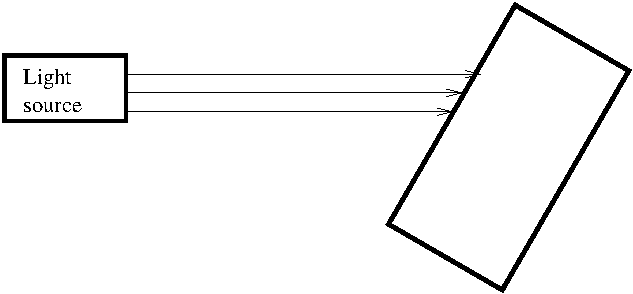
\includegraphics[width=3.5in]{lenses1/lensfig1.pdf}}


Put a piece of paper under the rectangle.  Trace the outline of the rectangle
on the paper.  Also, trace the path of one of the rays as it enters
the rectangle, and the same ray as it exits the other side.  Use
a straightedge to make sure your lines are straight.
Then remove the paper, and draw a straight line connecting the points
where the ray entered and exited the rectangle. 
You should end up
with a picture like this:

\answerspace{0.1in}
%\centerline{\epsfxsize 3in\epsfbox{figs/lensfig2.eps}}
\centerline{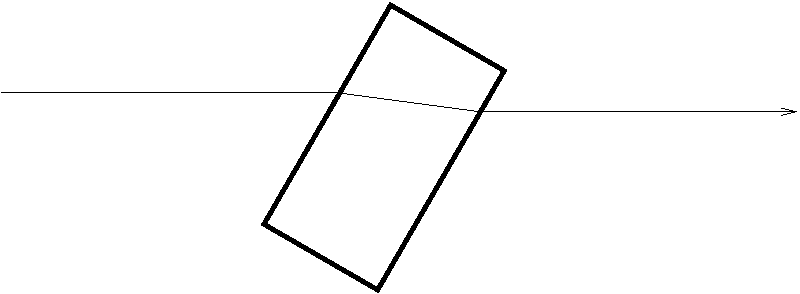
\includegraphics[width=4.5in]{lenses1/lensfig2.pdf}}



The light ray bends when it enters the plastic.  This phenomenon is
called {\it refraction}.  There is a rule called Snell's Law that
describes the amount of bending:
$$
\sin\theta_i=n\sin\theta_r.
$$
In this law, $n$ is a constant called the {\it index of refraction} of 
the material.  The angles $\theta_i$ and $\theta_r$ are called the
angle of incidence and angle of refraction.  They're defined to be the
angles the light ray makes with a line perpendicular to the surface
where the light ray entered the material, like this:

\answerspace{0.1in}
%\centerline{\epsfxsize 3in\epsfbox{figs/lensfig3.eps}}
\centerline{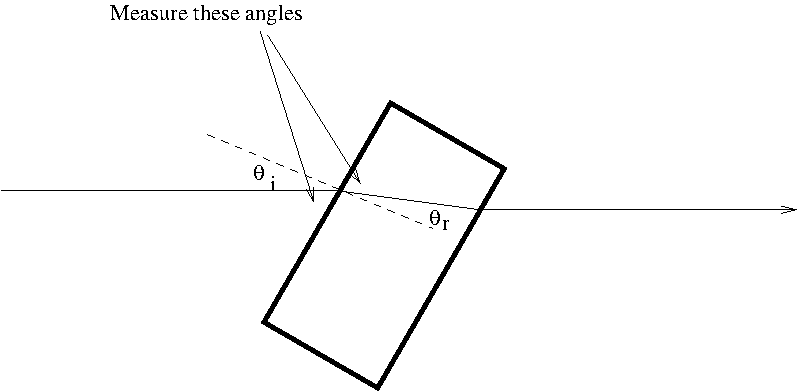
\includegraphics[width=4.5in]{lenses1/lensfig3.pdf}}

It's easier to measure the angles that the light ray makes with
the \textit{edge} of the rectangle, instead of the angle that it makes with
the \textit{perpendicular line}.  So measure the two angles
indicated by the arrows in the picture, and use them
to determine the angles $\theta_i$ and $\theta_r$.

\answerspace{1.5in}

Now use these angles in Snell's Law (the equation above) to determine
the value of the index of refraction $n$.

\answerspace{1.5in}

The value of $n$ is supposed to be the same no matter what incident angle
you choose.  To test this, rotate the rectangle so that the light
rays hit it at a different angle.  Repeat the procedure above to determine
$\theta_i$, $\theta_r$, and $n$.  Do you get roughly the same value of $n$ as
before?

\answerspace{3.0in}

\paragraph{Part 2: Total internal reflection.}
Once the light ray has entered the surface, it has to bend again
in order to get back out.  (That's why the rays that leave the rectangle
end up parallel to the ones that go in.)  Sometimes the rays can't bend
enough to make it back out, and in this case, they are reflected, bouncing
back and forth inside the material.  To see this, take the long, thin
rectangular piece of plastic, and arrange it so that one of the light
rays enters at a slight angle like this:

%\centerline{\epsfxsize 3in\epsfbox{figs/lensfig4.eps}}
\centerline{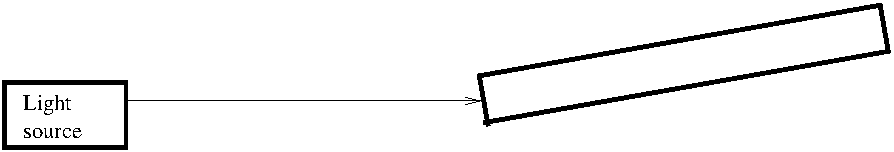
\includegraphics[width=5in]{lenses1/lensfig4.pdf}}



If you adjust the angles right, you should be able to see the light ray
bounce back and forth from side to side inside the plastic.  
Using total internal reflection, 
light signals can be transmitted over very great distances through
fiber optic cables.

\paragraph{Part 3: Lenses.}
A curved piece of refracting material can act as a lens, bringing
light to a sharp focus.  Lenses are found in your eyes, as well as
corrective lenses (eyeglasses or contact lenses), cameras,
microscopes, etc.  For this course, of course, the most important
application of lenses is in telescopes.  We'll examine how telescopes
work in future classes.  For the moment, let's just figure
out some general properties of lenses.

Take one of the three lenses labeled 1,2,3, and place it in front
of the light source.  You should see the light rays bending to
come (approximately) to a {\it focal point} on the far side of the lens.  
The {\it focal length} of a lens is defined to be the distance from the center
of the lens to the focal point.  Determine the focal lengths of all
three lenses.  (The easiest way to do this is to mark the focal point
on the white board, and also to mark the edges of the lens.  Then
you can remove the lens and measure the distance from the focal
point to the middle of the lens.)

\answerspace{2.5in}

These three lenses are all called {\it converging} lenses, because
they cause the light to converge to a point.  There are also {\it diverging}
lenses, which generally have concave rather than convex surfaces.  Put
the lens labeled 5, which is a diverging lens, 
in front of the light source and see what it does.
A diverging lens causes the light rays to spread out {\it as if} all the
rays were coming from a focal point on the same side of the lens
as the light source.

To see how this works, trace the paths of several of the rays 
after they exit the lens.  Also, mark the positions of the edges
of the lens.  Now remove the lens and, using a straightedge, extend
the rays {\it backward} until they come together at a single point.  
The distance from the center of the lens to this focal point is
called the focal length of the lens.  Measure the focal length
of this diverging lens.

\answerspace{1.0in}

\paragraph{Part 4: Combinations of lenses.}
Put one of the converging lenses (1,2,3) in front of the light source, and
then put another one of the converging lenses right in front of the first
one.  The two lenses should behave approximately like a single lens.
Is it a converging or a diverging lens?  How does the focal length of
the combined lenses compare with the focal length of the original
lenses?  (I'm not looking for a measurement here, just a general
observation.)

\answerspace{1.4in}

\pagebreak[2]
Try the same thing with a combination of a converging and a diverging
lens.  Does the combination behave like a converging lens or a diverging
lens?  

\answerspace{1.4in}

Remove the other lenses and place the lens labeled 4 in front
of the light source.  Is this a converging lens or a diverging lens?
Is its focal length larger or smaller than those of lenses 1,2,3,5?

\answerspace{1.4in}

Place the diverging lens (5) right in front of lens 4.  Does the combination
of lenses 4 and 5 behave like a converging lens or a diverging lens?

\answerspace{1.4in}

By now, you should have seen that sometimes a combination of a converging
and a diverging lens acts like a converging lens, and sometimes it
acts like a diverging lens.  There is a general rule for predicting,
for any given pair of lenses, which way the combination of the two
will behave.  Can you guess what this general rule might be?

\answerspace{0.7in}


\chapter{Image formation by lenses}


In this lab, you will examine how lenses form images.  In particular,
you will test the relationship between the location of the object
whose image is being formed and the location of the image.  Theoretically,
we expect that relationship to be
$$
{1\over p}+{1\over q}={1\over f}.
$$
Here $p$ is the {\it object distance} (distance from object to lens),
$q$ is the {\it image distance} (distance from image to lens, and $f$
is the {\it focal length} of the lens.

\bigskip

{\bf Part 1: Focal Length of a Lens}.

\begin{enumerate}

\item Arrange the light source appartus to produce parallel
rays of light across the surface of a piece of paper.
\item Place a convex lens in front of the
light rays.  Mark the lens position on a piece of paper, and trace
the path of the rays.
\item What is the distance from the center of the lens to the focal
point?  This is the focal length of the lens.

\vskip 1in

\end{enumerate}

\bigskip

{\bf Part 2: Image Formation}

\begin{enumerate}

\item Attach the light source to one end of the optical bench,
and place the lens partway down the bench.  Arrange the light
source so that the side with a circle and arrow drawn on it is
facing the lens.  This will be the ``object'' whose image we will
be examining with the lens.

\item Measure the length of the arrow.  We will call this $h_o$, meaning
``the height of the object.''

\vskip 1in

\item Adjust the lens and an index card until you see a clear, in-focus
image of the object on the card.  Measure the height of the image
$h_i$, the distance from lens to object $p$, and the distance from
lens to image $q$.  Record them in the table below.

\item Move the lens about 5 cm toward or away from the object, and move the
card until you get a clear image again.  Measure $h_i,p,q$ again.
Repeat until you have five sets of measurements.  For some, the image should
be closer to the lens than the object ($q<p$) and some should be 
the other way around ($p<q$).  (Note: make sure that the object
is always further away from the lens than the focal length.)

\vspace{0.3cm}
{\centering \begin{tabular}{|c|c|c|c|c|c|}
\hline 
~~~~~~~\( p \)~~~~~~~&
~~~~~~~\( q \)~~~~~~~&
~~~~~~~\( h_{i} \)~~~~~~~&
~~~~~~~\( \frac{h_{i}}{h_{0}} \)~~~~~~~&
~~~~~~~\( \frac{q}{p} \)~~~~~~~&
~~~~~~~\( f \)~~~~~~~\\
\hline
\hline 
&
&
&
&
&
\\
\hline 
&
&
&
&
&
\\
\hline 
&
&
&
&
&
\\
\hline 
&
&
&
&
&
\\
\hline 
&
&
&
&
&
\\
\hline
\end{tabular}\par}
\vspace{0.3cm}

\item For each observation, calculate and record the ratio of
image and object heights, $h_i/h_o$, and the ratio of image and
object distances, $q/p$.  Record these
in the table.  What can you conclude about these
quantities?

\vskip 1in

\item For each observation, use the formula at the beginning
of this lab to calculate the focal length of the lens, and record
it in the last column of the table.  Do these results appear consistent
with your measurement of the focal length in part 1?

\vskip 1in

\item Move the lens closer to the object, so that the object distance
is less than the focal length.  Note that there is nowhere you can
place the card to get a clear image.  Look through the lens at the
object.  Does the image appear to be larger or smaller than the actual
size of the object?  Does it appear to be closer or further away?

\vskip 1in

\item Suppose the object is extremely far away from the lens.
Based on your results, where would you expect the image to form?
(In other words, about what would you expect $q$ to be?)  Would
you expect the image to be large or small?

\vskip 1in

\item If the Sun is shining, take the lens outside along with
a piece of white paper, and try to form an image of the Sun on the
paper.  Are the results consistent with your predictions?

\vskip 1in

\end{enumerate}



\section{Refracting Telescopes}

\makelabheader

\bigskip
{\bf Part 1: Theory}

Suppose that you have a telescope made of two lenses.  The ``objective''
lens has a focal length of 10 centimeters, and the ``eyepiece'' lens
has a focal length of 1 centimeter.  A refracting telescope is constructed
so that the two lenses are separated from each other by a distance
equal to the sum of their focal lengths (11 cm in this case).  That
way, one of the focal points of the objective matches up with one
of the focal points of the eyepiece
The setup is something like this:

\medskip

%\centerline{\epsfbox{figs/telescopefig1.eps}}
\centerline{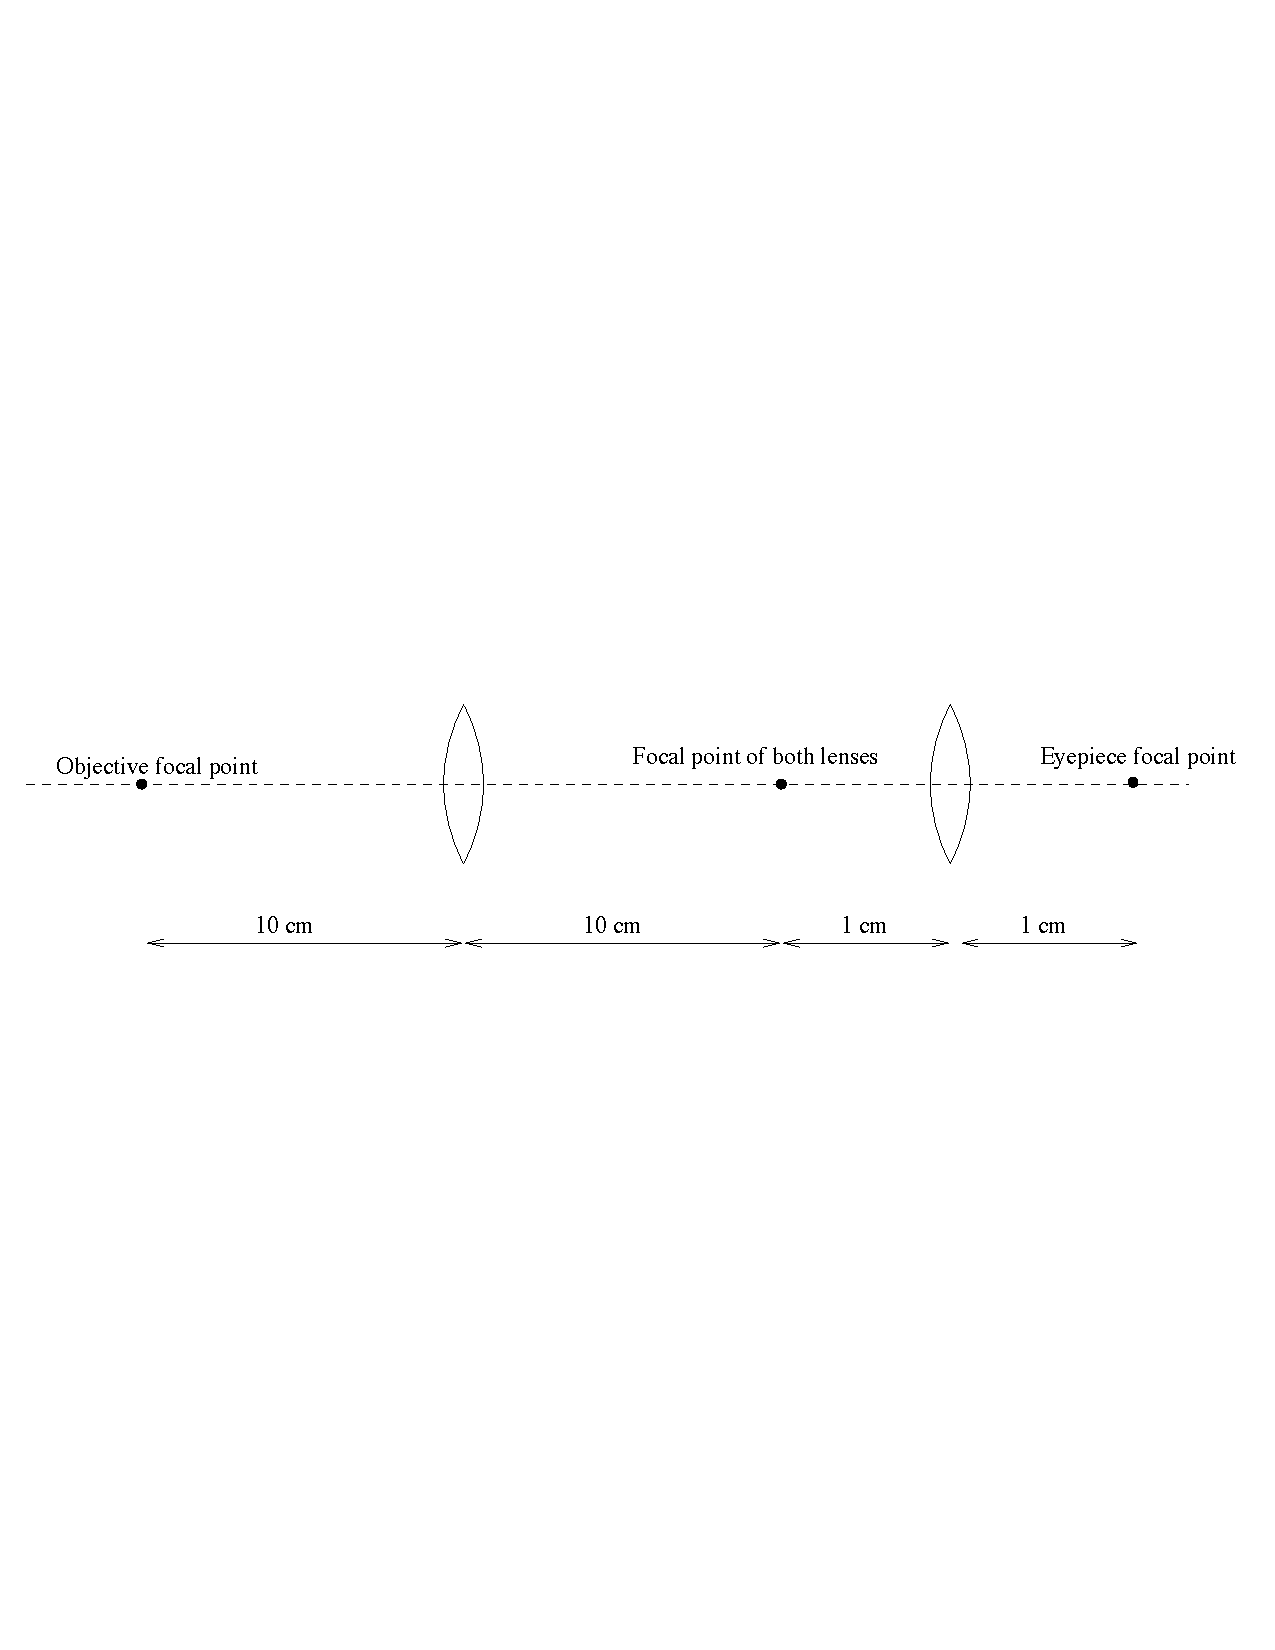
\includegraphics[width=\textwidth]{telescope/telescopefig1.pdf}}

\medskip

(Note that this picture is not to scale.)  The objective lens is on the
left, and the eyepiece is on the right.  The observer looks through
the eyepiece (not surprisingly) at a faraway object off to the left.

Suppose that you are using this telescope to look at an object that is
100 meters ($10^4$ centimeters) away.  We will work out where the
image of this object is produced, and how much it appears to be magnified.

The key facts that we'll need to do this are the rules you checked
in your last lab.  First, there's the relationship between the object 
position, the image position, and the focal length:
\begin{equation}
\frac{1}{p} + \frac{1}{q} = \frac{1}{f}.
\end{equation}
Second, there's the rule for the {\it linear magnification} of an image:
$$
\frac{h_i}{h_o}=\frac{q}{p}.
$$
Here $h_i$ is the height of the image produced by the telescope,
and $h_o$ is the height of the actual object.  The ratio of these two
is called the linear magnification $M$, so we'll write simply
\begin{equation}
M=\frac{q}{p}.  
\end{equation}
[Note: Often, the expression for the magnification is written with a minus sign
in it: $\displaystyle M=-\frac{q}{p}$.  It doesn't really matter for our purposes, though.]

In the calculations you're about to do, you'll be using known values of $p$ 
and $f$ and trying to find $q$.  So to make life simpler, take equation
(1) and solve it for $q$ in terms of $f$ and $p$.  (That is, rearrange
it so that it says $q=\ldots$.)  If you simplify this expression
as much as you can, you'll be less likely to make mistakes later.
(A good strategy is to isolate $\frac{1}{q}$ on one side of the equation,
then put the stuff on the other side over a common denominator, and
finally take the reciprocal.)  If you're not sure whether you've
got the right expression, show it to me.

\answerspace{2in}

Now suppose we have an object that is 100 m to the left of the telescope
above (so $p= 10^4$ cm).  The light passes through the objective lens
and forms an image (ignore the eyepiece for now).  Where is this
image?  Specifically, how far is it from the objective lens?  Also,
is it a real image or a virtual image?  When figuring out the
location of the image, record an answer in centimeters with at least
three digits after the decimal point.  (In other words, record
your answer to an accuracy of 0.001 cm.)

\answerspace{1in}

Mark the approximate location of this image with an $X$ on the diagram
above.
How far is this image from the eyepiece lens?  Again, record your answer
to an accuracy of 0.001 cm.

\answerspace{1in}

Calculate the linear magnification of this image using equation (2).
This should be a number between 0 and 1.  It indicates the factor
by which the image is smaller than the original object.

\answerspace{1in}


Now we want to figure out the effect of the eyepiece lens.  The big
idea here is that we treat the {\it image} produced by the objective
lens as if it were the {\it object} for the eyepiece lens.  That is,
we pretend that the image is a real thing that the eyepiece is examining.
That means that the answer to the previous question (distance
from the image to the eyepiece lens) becomes the new {\it object distance}
$p$.

Is the image produced by the eyepiece a real image or a virtual image?

\answerspace{1in}

How far away is the image produced by the eyepiece?
(When you calculate this, your answer for $q$ will come out negative.
That's OK: you can ignore the minus sign.  It just indicates that
the image is virtual.)

\answerspace{1in}

Now you know where the image will appear to be when you look through
the eyepiece.  Calculate the ratio of the distance to the original
object to the distance to the final image.  This is how many
times closer the telescope makes the object appear.

\answerspace{1in}

Use equation (1) to calculate the linear magnification of the image produced by 
the eyepiece.  This should be a number greater than 1.  It indicates
the factor by which the eyepiece has magnified the image.

\answerspace{1in}

The {\it overall linear magnification} of the telescope is the product
of the magnification produced by the objective lens and the magnification
produced by the eyepiece lens.  What is the overall 
linear magnification of this
telescope?

\answerspace{1in}

This number tells you how many times larger or smaller the final image
is than the original object.  
You should have found that this number is less than 1, which means
that the final image is actually {\it smaller} than the object.
That may seem surprising since we expect a telescope to make
things look bigger, not smaller.  What's going on here?

The point is that this linear magnification tells you how the
actual size of the image and object compare.  If you want to know
how big an object {\it looks}, you need to consider their
angular sizes.  The ratio of the angular size of the
final image to the angular size of the original object
is called the {\it angular magnification}.
What is the angular magnification of this telescope?

Hint: The angular size depends on both the actual size and the
distance.  You've already worked out what effect the telescope has on
the distance of the image (as compared to the object), and what effect
it has on the size of the image (as compared to the object).


\answerspace{1.5in}

There is a general rule that says that the angular magnification
of a telescope is equal to the ratio of the focal lengths $f_{\rm objective}/
f_{\rm eyepiece}$.  Is that true in this case?

\answerspace{1in}


{\bf Part 2: Constructing a Telescope}

In this part of the lab, you will use two lenses and some cardboard tubes
to construct a telescope.  

Determine the focal lengths of the two lenses, by any means you 
can think of.

\answerspace{1in}

According to the rule at the end of the last part, the angular
magnification of a telescope is the ratio of the focal lengths.
What is the angular magnification of a telescope constructed with
these lenses?

\answerspace{1in}

Insert the lenses into the tubes and adjust the distance between the lenses
until the telescope gives a sharply-focused image of faraway objects.

What is the orientation of an object as seen in the telescope?  Are
they upside-down?  Are they reversed left-to-right?

\answerspace{1in}

\pagebreak[2]

Stand in a location where you can see the eye chart posted on the wall.
Adjust your distance from the eye chart until you can just barely
read the F at the top of the chart (without using the telescope).
Now look at the chart with the telescope.  Which row is the
smallest row you can read using the telescope?  How many times
smaller is this row than the F at the top?  (The sizes of the letters
in each row are printed at the right of the chart.)
Compare this ratio with the angular magnification you calculated
for the telescope.  Do the results make sense?

\answerspace{1in}


\section{Stefan-Boltzmann Law}

\makelabheader


\paragraph{Introduction.}
Stars (and other astronomical objects) emit a lot of their energy
in the form of \textit{thermal radiation}. To understand how these objects
work, we need to know how much energy they emit. In this lab, you'll
examine the relationship between the amount of \textit{power} (that is,
energy per time) emitted
by an object and the object's \textit{temperature}.

The apparatus for this experiment consists of a lamp and a radiation sensor.
The lamp will be hooked up to a power supply, and the radiation sensor
is attached to a meter that indicates the intensity of light
striking it.

\centerline{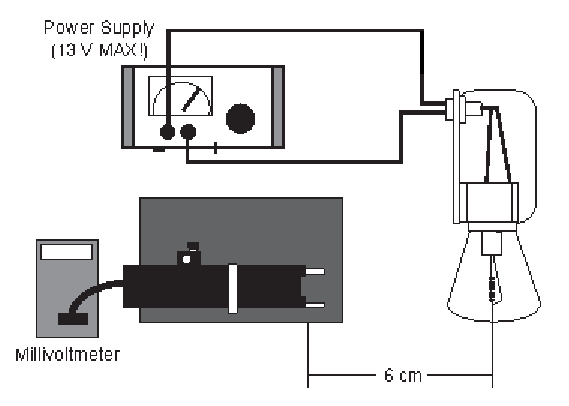
\includegraphics{stefan/stefan1.pdf}}

By changing the voltage being applied to the lamp, we can change its
temperature. The radiation sensor then tells us how much power is being
emitted at any given temperature.

We're going to want to know how the power depends on the temperature of the
lamp filament. We can't conveniently attach a thermometer to the filament,
so we have to get the temperature another way, namely by measuring
the filament's \textit{resistance}, which depends on the temperature
in a known way. Here's how this works.

Suppose we apply a certain number of volts $V$ to the lamp. That voltage
will cause electric current to flow through the lamp. We'll measure
the amount of current, which is traditionally called $I$ (for some reason). 
The resistance is the ratio of these two:
$$
R=\frac{V}{I}.
$$
The value of $R$ increases in a known way as the temperature goes
up, so by keeping track of $R$ we'll be able to keep track of the
temperature.

\pagebreak[3]

\paragraph{Gathering the data.}
The first thing you'll need to know is the resistance $R$ of the filament
when it's at room temperature. We'll do this by applying a small voltage
to the lamp, and recording the amount of current that flows. If we keep
the voltage small, we can assume that the lamp won't heat up very much,
so we can use these values to figure out the resistance at 
room temperature.

Connect the lamp to the power supply as shown in the diagram.
Turn the voltage knob all the way to zero (counterclockwise), and turn
the current knob up (clockwise). Now turn on the power supply.
The voltage display on the power supply should read zero. Turn up the voltage
knob gradually until it reads about 0.5 volts.

At this point, the power supply is supplying a small amount of energy to push
a small amount of current through the lamp. It's not enough to heat up
the filament significantly or to make the lamp glow. 
Record the voltage ($V$) and current ($I$) readings on the power supply here. The voltage 
should be 0.5 V, and the current is some number of ``amperes'' (A).

\answerspace{0.3in}
$$
V=\qquad\qquad\qquad\qquad\qquad
I = \qquad\qquad\qquad\qquad\qquad\ 
$$

\answerspace{0.3in}

Use the rule $R=\frac{V}{I}$ to determine the resistance. 
The unit of resistance is called the ``ohm'' and is written $\Omega$.

\answerspace{0.3in}
$$
R_{300\,{\rm K}}=
$$
\answerspace{0.3in}

You might wonder why we call it by the strange name $R_{300\,{\rm K}}$.
The reason is that this is the value of the resistance at room temperature, 
which corresponds to a 
temperature of about 300 kelvin. 

Now that you have this, you can start taking measurements when the lamp
is actually glowing. First, make sure that the lamp is at the same height
as the radiation detector, and the distance between the two is about 6 cm.
The exact distance doesn't matter, but it's important that it not 
change once you start measuring. Make sure that the detector is facing
directly toward the lamp and there are no other bright light sources
in its path. The radiation sensor should be hooked up to the
voltmeter's inputs labeled COMMON and V/$\Omega$, and it should 
be set to read DC voltage. That setting on the meter's dial will
probably look like a V with straight lines (not a wavy line) 
next to it or above it.
Check with me to see if you've got everything wired up correctly.

Once you're ready, turn up the voltage dial gradually until it reads 2 volts.
You should see the lamp glowing faintly.

In the data table at the end of this lab, record the voltage $V$ (which is 2 V),
the current $I$ from the display on the power supply,
and the reading on the voltmeter
attached to the radiation sensor. The last number is a measure
of the power being radiated by the lamp, so we'll call it $P$. 
Record these values
in the first row of the table on the last page of this lab. (Leave
the other columns in this table blank for now.)

Once you've done this, repeat for voltages of 4, 6, 8, 10, 12 V.

You should expose the radiation sensor to the lamp light only briefly
when you're making each power measurement. In between measurements, place 
sheets of insulating foam between the lamp and the sensor, with the silvered
surface facing the lamp, so that the temperature of the radiation sensor
stays fairly constant.


\paragraph{Analyzing the data.}
You'll need to determine the temperature of the filament during each of these
measurements, by filling in the remaining columns in the data table. Here's
how. 

First, find the value of the resistance for each row, using the rule $R=\frac{V}{I}$. 

The temperature is determined by how this resistance compares with its
value at room temperature, so compute the ratio ${\frac{R}{R_{300\,{\rm K}}}}$
for each row.

The graph near the end of the lab 
shows how this ratio is related to temperature.
For each row in the table, use the graph to determine the value of 
temperature corresponding to the resistance ratio you've determined.
(Read across the graph at the height corresponding to the ratio.
When you hit the curve, go straight down to get the temperature.)

Once you've done this, the data table should be filled in.
Now we want to graph it, using \textit{Excel}. Appendix B of your
lab manual contains some information about making graphs in \textit{Excel}.
Create an \textit{Excel} data table with two columns, $T$ and $P$. (Put
$T$ on the left.) Following the instructions in Appendix B.2, make
a graph showing how $P$ depends on $T$. 

You should find that the power goes up as the temperature goes up.

We want to see what sort of mathematical relationship matches this graph. 
Try adding a ``trendline'' to the chart, following the instructions
in Appendix B.3.
This shows the straight line
that matches the data as well as possible. Does a straight line look
like a good fit to this set of data?

\answerspace{1in}

Double-click on the trendline to get various options to customize it.
You should see various options such as ``Exponential,'' ``Linear,'' etc.
These replace the straight-line relationship with various other 
mathematical relationships. You can try all of these out to see
which ones look like a good match to the data.

In the end, we'll be most interested in the one called ``Power.'' Select
this trendline option, and also check the box that says ``Display
equation on chart.'' What this does is to find the best-fitting mathematical
relationship of the form $y=\mbox{(something)}\times x^{\mbox{(something)}}$
between the two quantities in the graph. In our case, $x$ and $y$
are $T$ and $P$ respectively.

According to \textit{Excel}, what is the best-fitting value
of the exponent (the power of $x$) in this relationship?

\answerspace{1in}

What do we expect this exponent to be, according to the Stefan-Boltzmann
Law? (If you don't remember this from your reading, you can look it up.)

\answerspace{1in}

Do your data agree reasonably well with the Stefan-Boltzmann Law?

\answerspace{1in}


\centerline{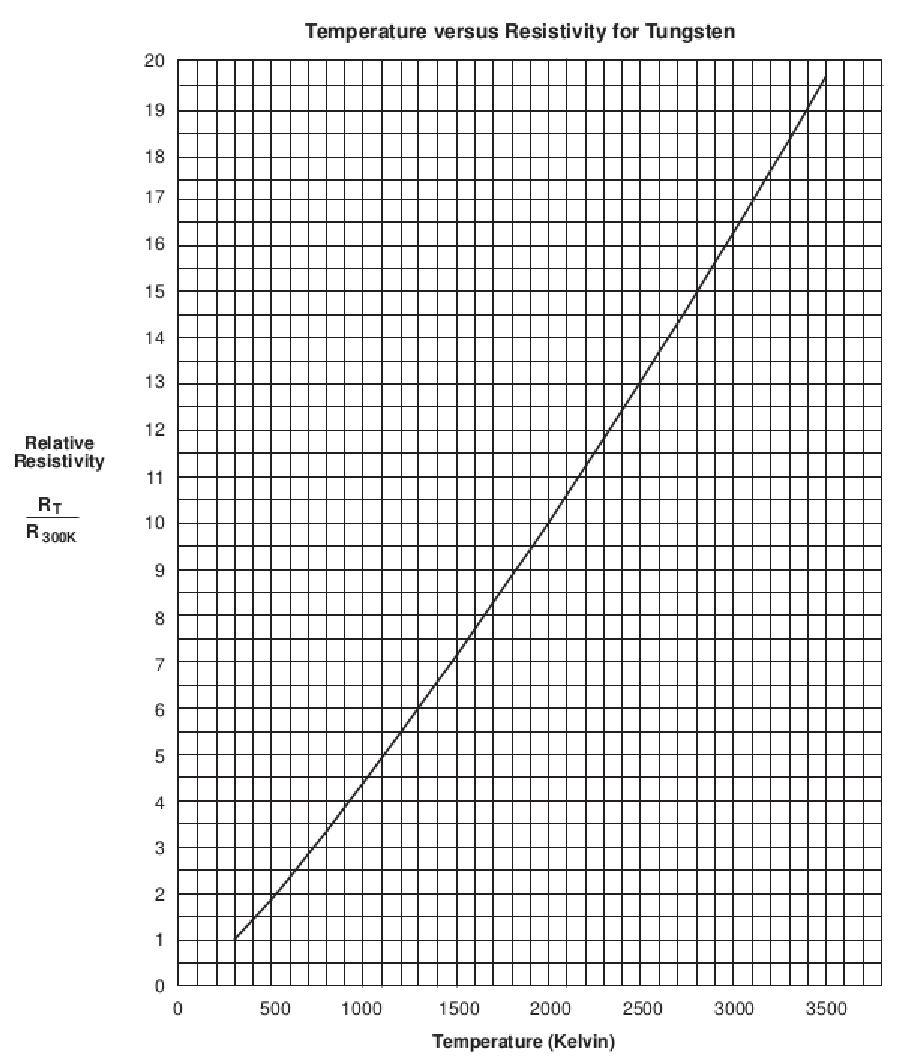
\includegraphics{stefan/stefan2.pdf}}

\vfill
\pagebreak[4]


\begin{center}
\begin{tabular}{|p{0.8in}|p{0.8in}|p{0.8in}|p{0.8in}|p{0.8in}|p{0.8in}|} \hline
$V$ (volts) & $I$ (amps) & $P$ (mV) & $R$ ($\Omega$) & $R/R_{300
\,{\rm K}}$\ & $T$ (K) \\ \hline
\ & \ & \ & \ & \ & \ \\
\ & \ & \ & \ & \ & \ \\
\ & \ & \ & \ & \ & \ \\
\ & \ & \ & \ & \ & \ \\ \hline
\ & \ & \ & \ & \ & \ \\
\ & \ & \ & \ & \ & \ \\
\ & \ & \ & \ & \ & \ \\
\ & \ & \ & \ & \ & \ \\ \hline
\ & \ & \ & \ & \ & \ \\
\ & \ & \ & \ & \ & \ \\
\ & \ & \ & \ & \ & \ \\
\ & \ & \ & \ & \ & \ \\ \hline
\ & \ & \ & \ & \ & \ \\
\ & \ & \ & \ & \ & \ \\
\ & \ & \ & \ & \ & \ \\
\ & \ & \ & \ & \ & \ \\ \hline
\ & \ & \ & \ & \ & \ \\
\ & \ & \ & \ & \ & \ \\
\ & \ & \ & \ & \ & \ \\
\ & \ & \ & \ & \ & \ \\ \hline
\ & \ & \ & \ & \ & \ \\
\ & \ & \ & \ & \ & \ \\
\ & \ & \ & \ & \ & \ \\
\ & \ & \ & \ & \ & \ \\ \hline
\end{tabular}
\end{center}

\section{Solar Radiation and the Greenhouse Effect}

\makelabheader

\bigskip

The Earth (like the other planets) is warmed by
sunlight.  The Earth also radiates energy into
space, mostly in the form of infrared radiation.
On average, the amount of radiation received from the Sun
must equal the amount of radiation emitted by the planet.  After 
all, if the Earth emitted less radiation into space than it 
received from the Sun, then its temperature would keep going up;
and if it emitted more radiation than it received, it would keep
cooling down.  Since the temperature of the Earth is fairly stable
over the years, the radiation coming in from the Sun must balance
the radiation being emitted.

Note: You've doubtless heard about global warming, so you may
wonder how I can get away with saying that the temperature
of the Earth is fairly stable. Global warming does mean there's
an imbalance between the incoming and outgoing radiation, but
it's very slight. Although that slight difference is enough to have
major consequences for the climate, it's small enough that we can safely
ignore it in the calculations we're about to do.

In this lab, you will use this idea to form an estimate of the
temperature of the Earth.  Specifically, you will calculate
the total amount of solar power striking the Earth's surface.
Then you will assume that the Earth radiates that same amount
of power back into space.  Assuming that the Earth radiates
as a blackbody, you can use the Stefan-Boltzmann law to 
relate the radiated power to the temperature and so calculate
the temperature of the Earth.

This calculation depends on one important assumption: that the
Earth radiates like a blackbody.  That assumption is wrong,
so our calculated temperature will not match the actual
temperature of the Earth.  In particular, a phenomenon
known as the ``greenhouse effect'' blocks some of the
Earth's radiation from escaping into space.  The results
of this calculation will give an indication of how important
the greenhouse effect is here on Earth.

Let's get started.
Remember that the Sun's luminosity is
$$
L_{\odot}=3.86\times 10^{26}\,{\rm W}.
$$
A watt (W) is a unit of power equal to a joule per second.
This is the total amount of power emitted by the Sun in all directions.
The first thing we want to do is to figure out how much of this
power strikes the Earth.

Consider an imaginary sphere centered on the Sun with a radius
of 1 A.U.  All of the radiation that leaves the Sun must pass through
this sphere.  Calculate the amount of radiation that strikes each square
meter of this imaginary sphere's surface by dividing the Sun's luminosity
by the sphere's surface area.  Remember that the surface area of a sphere
of radius $R$ is
$$
A=4\pi R^2.
$$
Remember that an A.U. is $1.49\times 10^{11}$ meters.
Give your answer in units of watts per square meter (W/m$^2$).

\answerspace{1in}

\pagebreak[4]
Now work out how much solar radiation strikes the Earth.  To do this,
note that the Earth covers up a small circular patch of that great big
imaginary sphere.  The amount of radiation striking the Earth will equal
the amount striking that small circular patch.  Recall that the area
of a circle is $\pi R^2$.  The radius of the Earth is 6380 kilometers.
What is total amount of solar radiation
striking the Earth?  Give your answer in watts.

\answerspace{1.5in}

The Earth doesn't actually absorb all of that energy; some of it
is reflected into space.  The fraction of energy that is reflected
by an object is called the object's {\it albedo}.  Measurements of Earth
from space have shown that the Earth's albedo is 0.35, meaning that it
reflects 35\% of all the radiation that hits it back into space and absorbs
the rest.  

What is the total amount of solar radiation {\it absorbed} by the Earth?

\answerspace{1in}

This number must equal the amount of radiation emitted by the Earth.
Assume for the moment that the Earth emits radiation as a blackbody.
That means that it obeys the Stefan-Boltzmann law,
$$
F=\sigma T^4.
$$
Recall that $\sigma=5.67\times 10^{-8}$ W/(m$^2$ K$^4$).
Also, remember that the flux $F$ in the Stefan-Boltzmann law
is the power radiated per area (watts per square meter).  To get
the total power radiated by the Earth, therefore, we should
multiply the flux by the surface area of the Earth.  As noted
earlier, the surface
area of a sphere is $4\pi R^2$, so the total
power radiated by the Earth
is
$$
L_{\oplus}=4\pi R^2\sigma T^4.
$$
Here $\oplus$ is the symbol for the Earth.  $L$ stands
for ``luminosity,'' which is what we always call the total
amount of power emitted by an object.  $R$ is the radius
of the Earth, and $T$ is the temperature.

Set this expression equal to the total amount of solar power
being absorbed by the Earth and solve for the temperature $T$.
Your answer will come out in kelvin.  Subtract 273 to convert 
it to degrees Celsius.

\answerspace{1.5in}

Does this seem like a reasonable estimate of the Earth's 
actual average temperature?

\answerspace{1in}

The main thing that went wrong in this calculation is the assumption
that the Earth radiates as a blackbody, also known
as a  ``perfect radiator.''
Suppose that something in the Earth's atmosphere is blocking
radiation from getting out, so that it's not a perfect radiator.
Then the amount of radiation leaving the Earth will be less than 
the amount calculated from the Stefan-Boltzmann law.  This
alters the balance between incoming and outgoing radiation, resulting
in an increase in temperature.

Carbon dioxide and other gases in the Earth's upper atmosphere reflect some of
the Earth's infrared radiation back down to the planet, preventing it from
escaping into space.  This ``greenhouse effect'' means that
the Earth is not a perfect radiator, and it is why
the Earth is warmer than your calculation above would indicate.

The greenhouse effect is responsible for climate change, so
we think of it as a bad thing these days,
but without it, the Earth would be uninhabitably cold!  The
problem we face now is that human activity has led to
an {\it increase} in the
greenhouse effect, altering the balance that existed for 
many millennia before we started altering the composition of the
atmosphere.

Venus is an interesting example of the greenhouse effect.
Follow the same steps as above to figure out what
the surface temperature of Venus would be in the absence of
a greenhouse effect.  Here's some useful information about Venus:

\begin{itemize}
\item Distance from Sun to Venus: 0.723 A.U.
\item Radius of Venus: 6050 km.
\item Venus's albedo: 0.65.
\end{itemize}

You'll also need to know the luminosity of the Sun ($3.86\times 10^{26}$ W)
and the number of meters in an A.U. ($1.49\times 10^{11}$ m).

\vfil

Probes of Venus indicate that its surface temperature is about 700 K
(430~$^\circ$C, or 800~$^\circ$F).  Would you say that the
greenhouse effect is more important on Venus than on Earth or 
vice versa?

\answerspace{1in}
\eject





\section{Energy Flow in the Sun}

\makelabheader

In this lab, you will examine how the energy produced in the core
of the Sun makes it out to the surface.  The nuclear reactions in
the core of the Sun produce photons, which eventually make their way
to the surface of the Sun.  This process takes a long time because
the photons undergo frequent collisions with ionized atoms
in the solar interior.  These collisions cause the photons to
bounce around in random directions instead of zooming
straight out.

You will use simulation software to examine the process by which
these photons make it out of the Sun.
If it's not already running, 
start up the ``energy flow out of the Sun'' application on the lab
PC and log
in.  It doesn't matter what you enter for names and table number.\footnote{For 
boring technical reasons, this program has to run inside of a 
``virtual machine'' that's set up on the lab computers. I'll make sure
that it's all set up before class. This may mean that the application
may run in a window inside of another window, which looks a little funny
but doesn't make a difference in the end. }

\medskip

{\it Part 1: Photons moving through a gas.}

Select ``Interaction'' under the ``Simulation'' menu, and click
``Run.''  This shows what happens to photons as they pass through a
dense gas.  The stationary circles represent atoms in the gas, and the
smaller white circles represent photons.  You should imagine that
there is a source of photons off to the left somewhere, sending
photons into the gas.  These photons have the correct amount of energy
to correspond to one of the spectral lines of the atoms.  That means
that when a photon hits an atom, it is very likely to be absorbed,
sending the atom into an excited state.  The atom quickly drops
back down to its original state, re-emitting the photon in a new direction.
The end result is that the photon undergoes a ``random walk'': instead
of moving in a straight line, it bounces around making frequent
changes in direction.

Stop the simulation.  Under ``Photon Type,'' select ``Continuum,'' and
restart the simulation.  With this setting, the photons now have an
energy that does {\it not} correspond to a spectral line of these
atoms.  This means that the atoms cannot absorb the photons, so the
photons usually just pass right through.  

On rare occasions, a photon
with the wrong energy can bounce off of an atom, as you'll see if you 
let the simulation run for a while.

The {\it mean free path} is the average distance that a photon travels
before it bounces off of an atom.  Which has a longer mean free path,
the continuum photons or the line photons?

\answerspace{1in}

If the continuum photons {\it never} bounced off of atoms (as opposed
to rarely doing so), what would their mean free path be?

\answerspace{1in}

Here's an important thing to realize for the rest of the lab:
Throughout most of the interior of the Sun, the gas is ionized,
meaning that the electrons are stripped off of the protons.  Ionized
gas is capable of interacting with photons of {\it all} wavelengths,
not just specific ones.  That means that {\it in the interior of the
Sun, all photons behave like the ``line'' photons in this simulation.}

{\it Part 2: Photon Diffusion in the Sun}.

Click ``Return'' to get back to the main menu.  Under ``Simulation,'' 
go to ``Flow'' and then to ``1 Photon.''  
This simulation shows the path of a single photon as it makes its
way out from the center of the Sun.  Click ``Run'' a few times to 
see how the photons behave.  Go to ``Parameters'' and check the ``Yes''
box under ``Trails.''  This will cause the photon's path to be
visible as it makes its way out.

In the ``Parameters'' menu, you can also vary the size of the Sun.
Select \# of Layers.  It should initially be 20.  Change that value to 40
and try running the simulation again.  You should see that the Sun
has gotten larger, and not surprisingly, it takes more time for the photons
to make their way out.

In this model of the Sun, each ``layer'' of the Sun has a thickness
equal to the mean free path of the photons.  That is, on average,
a photon can make it in or out of the Sun by only one layer between
bounces.  The more layers there are, the more times a photon is likely
to bounce on its way out, and so the longer it will take to get out.
In fact, there is a general rule relating the number of layers to the
time it takes photons to get out, which you will now determine.

Because the photons bounce around randomly, some get out faster than others.
We're going to be interested in the time it takes the \textit{average}
photon to get out, so we'll want to run the simulation with a bunch of photons
all at once. Go to the ``Simulation'' menu, and click ``Flow'' and then
``Diffusion.'' This will behave just like the simulation, but with many photons.


Under ``Parameters,'' you can set the number of layers and the number of
photons. Set the number of layers to 10, and the number of photons to 200.
Start the simulation, and let it keep going until all 200 photons have escaped
from the Sun.
record
the average number of interactions required for a photon to make it out.

\answerspace{1in}


Repeat the process for a 20-layer Sun.  


\answerspace{1in}



Do it one more time, this time for a 30-layer Sun. This one will take
a little while!

\answerspace{1in}

Based on these results, take a guess about the mathematical relationship
between the number of layers and the average number of interactions
taken to get out:

\answerspace{1in}

Ask me if you're not sure whether your guess is right.

This relationship only tells you about the {\it average} time it takes
a photon to get out.  As you've seen,
some photons are faster than average, and some
are slower. Let's do one more simulation to get a feel for this.

Set the number of layers to 25, and the number of photons to 1000,
and start the simulation running.  After how many interactions
does the first photon make it out?

\answerspace{1in}

Wait until most of the photons have escaped.  What is the average number
of interactions of all the photons?  Is this consistent with your
expectations based on the mathematical relationship you guessed above?

\answerspace{1in}

The graph in the lower part of the window shows the number of photons
escaping the Sun as a function of time.  The yellow line is the time
when the number of interactions is $n^2$ (the square of the
number of layers).  Sketch a copy of the graph below.

\answerspace{1in}

This graph shows that quite a few photons (well over half) make it out
in less than the average time, but some take much, much longer than that.

\medskip

{\it Part 3: Numbers for the actual Sun.}

In these simulations, the number of layers is very small.  In the actual
Sun, the photons can travel only a very short distance before
scattering (that is, the ``mean free path'' is small).  Since a ``layer''
is supposed to be only as thick as the mean
free path, a realistic model of the Sun would have many, many layers.
In this portion of the lab, you'll work out some rough numbers for
the actual Sun.

Based on the physical laws governing interactions between photons
and electrons, scientists estimate that the mean free path
of photons inside the Sun is about a tenth of a millimeter ($10^{-4}$ meters).
The Sun's radius is about 700,000 kilometers.  If
each ``layer'' has a size equal to the mean free path, how many layers
does the Sun consist of?

\answerspace{1in}

Based on the relationship you found earlier between the number of layers
and the number of interactions (bounces), how many interactions
will an
average photon undergo on its way out of the Sun?

\answerspace{1in}

The average distance a photon travels between interactions
is equal to the mean free path, and of course, photons travel at the
speed of light (300,000 km/s).  What is the average time between
interactions for a photon in the Sun?

\answerspace{1in}

From the average time between interactions and the total number of
interactions, determine how much time it takes the average photon to
make it out of the Sun.  Convert your answer into years.

\answerspace{1.5in}

If the nuclear fusion reactions powering the Sun were to somehow stop
tomorrow, would we notice an immediate reduction in the Sun's
luminosity?

\answerspace{1in}

Is there any way we could tell if the nuclear reactions in the Sun
stopped tomorrow?



\section{Parallax}

\makelabheader

{\bf Introduction.}

Parallax is the method used to find the distances to the closest
stars.  It is the first step in the ``distance ladder'' used to find
distances to other stars and ultimately to other galaxies.  In this
lab, you will use the method of parallax to determine the distance to a
nearby object: one of the classroom windows.

Here's the big idea behind parallax measurements.  Suppose you want
to measure the distance to the star in the drawing below.
You observe
the apparent position of the star from two locations A and B.  The directions
you have to look in order to see the object from the two locations
are slightly different, and the amount of difference can be represented
by the angle $\theta$.  If you can determine $\theta$, then you can
use the small-angle formula to determine the distance to the object.

The small-angle formula says that
$$
s = \left(\frac{2\pi}{360^\circ}\right)\theta D.
$$
Here $s$ is the distance between the two observation points, and 
$D$ is the distance to the object.\footnote{This is the version 
of the small-angle formula that has $\theta$ in degrees.  That's
the version that's most useful in this lab.  If you measure angles
in arc-seconds instead, then you use the version of the
formula that has the number $206\,265$ in it.}

(By the way, when we first learned the small-angle formula, we said
that $s$ was the separation between two different objects being
observed, not the separation between two different observation points.
We're now applying the formula to a different situation, but since the
geometrical setup is the same, the same formula works.)

The next question is how to measure $\theta$.  {\it In principle}, we could
measure $\theta$ like this:
\begin{enumerate}
\item Put the telescope at point A and point it at the star.
\item Move the telescope from point A to point B, being {\it very careful}
not to rotate it as you move it.
\item Once the telescope is at point B, rotate it until it is again pointing
at the star.  Measure the angle through which you had to turn the
telescope.  This is $\theta$.
\end{enumerate}
Here's a picture of the various angles:

\centerline{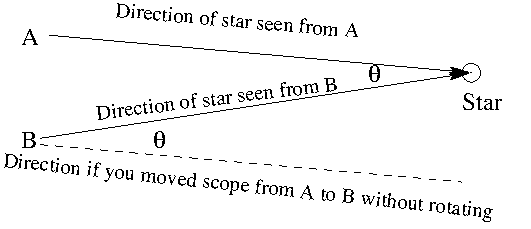
\includegraphics[width=4in]{parallax/parallax.pdf}}

Although there is nothing wrong with this method in principle,
in practice, it's quite inaccurate.  The reason is step 2: it's very hard
to make sure that you didn't jostle the telescope and rotate it just a little
bit when you were moving it.  Since parallax angles are very small, even
a slight error in this step will ruin the method.  So {\it the method above
is no good in practice}.

\pagebreak[2]

To make the method work, we need to measure the shift in the angular
position of the star by comparing it to some much more distant background
objects.  Here's the idea:
\begin{enumerate}
\item Put the telescope at point A.  Point the telescope at the
star.
\item Rotate the telescope until it points at a particular {\it background
object}.  Measure the angle through which you had to turn the telescope
to do this.  The result is the {\it angular separation} between the
star and the background object.  Let's call this angle $\alpha$.
\item Move the telescope to point B (without worrying about whether
you're rotating it as you go).
\item Point the telescope at the star, then at the same background
object as before.  Measure the angular separation this time, and call
it $\beta$.
\item The parallax angle $\theta$ is just the difference between
$\alpha$ and $\beta$.
\end{enumerate}
The picture below illustrates the various angles in this
method.  The main point is that
the background object is presumed to be extremely far away (much further
than the star).  This means that the lines of sight to the background
object from the two locations are essentially parallel to each other.

\centerline{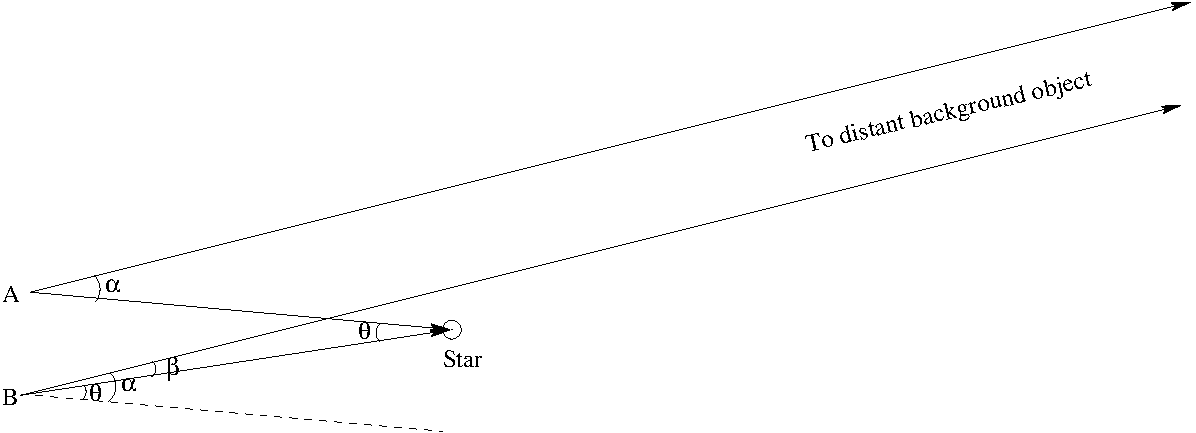
\includegraphics[width=6in]{parallax/parallax2.pdf}}


\bigskip

{\bf Procedure.}

The ``star'' in this lab will be the vertical divider separating
two panes of the windows at the side of the classroom.  Arrange
the telescopes so that you have a clear view of the ``star.''
Put down a couple of pieces of masking tape to mark the location
of the telescope.  You'll need these later when you determine
how far you moved the telescope.  You can mark the locations
of any convenient points on the telescope base.

(Incidentally, the telescopes we're using here are the ones on the
spectroscopes.  We're not using the ``slit'' side of the spectroscopes
at all in this lab; we're just using the ``telescope'' side.  So 
just set up the apparatus so that the slit is off out of the way, and
ignore it.)

Rotate the telescope until the ``star'' is centered in the field of view.
Use the crosshairs to make sure it's lined up accurately.
Record the angle made by the telescope.  If you forget how to read
the Vernier scale on the telescope base, ask me.

\answerspace{1in}

Look through the telescope, and choose a faraway ``reference object.''
This should be something easily identifiable and far away (outside
of the building, and preferably across the street).  It should also
be close to, but not quite, the same direction as the ``star.''
Good choices are tree trunks, signs, or lamp posts.

Rotate the telescope until the reference object is centered on the crosshairs,
and record the angle made by the telescope now.

\answerspace{1in}

Subtract these two angles from each other.  The result is $\alpha$,
the angular separation between the ``star'' and the reference
object.  (If I were you, I would convert the angles from degrees
and minutes into a decimal number of degrees before subtracting.
For instance, I'd convert $42^\circ\ 20'$, into $42.33^\circ$,
by using the fact that a minute is $\frac{1}{60}$ of a degree.)

\answerspace{1in}

Move the telescope over about 15 centimeters or so.  (The exact amount
doesn't matter.)  Move it in a direction perpendicular to the direction
of the ``star,'' not towards or away from the star.
Mark the new position with masking tape again.

Look through the telescope.  You should notice that the position
of the ``star'' relative to the background objects has shifted
a bit.  That's parallax.

Repeat the procedure above: Measure the angular position of the
star and the angular position of the reference object (same object
as last time!).  
\answerspace{1.8in}

\pagebreak[3]
What is the parallax angle $\theta$?

\answerspace{1in}

Using a ruler and your masking tape marks, measure the distance between
the two observation points A and B.

\answerspace{1in}

Now you have all the information you need to determine the distance to
the ``star.''  What is it?

\answerspace{1in}

Use a tape measure to determine the actual distance.

\answerspace{1in}

Do you think your results are reasonably accurate?  What
do you think the main sources of error are in this method?







%\chapter{Stellar Parallax}

This lab uses the Virtual Astronomy Laboratory software to perform
simulated observations of stellar parallax.  In fact, the writeup
is lifted (with permission, of course) straight from the manual
that came with the software.

Start up the 
{\it Virtual Astronomy Laboratory} application,
and select option 19, {\it Stellar
Parallax}.  We'll be skipping the Preliminary Exercises and going
straight to the Stellar Parallax part.  

\newpage

\hskip-0.5in
\includegraphics[height=10in]{val/parallax1.eps}

\hskip-0.5in
\includegraphics[height=10in]{val/parallax2.eps}

\hskip-0.5in
\includegraphics[height=10in]{val/parallaxp65.eps}

\hskip-0.5in
\includegraphics[height=10in]{val/parallax3.eps}

\hskip-0.5in
\includegraphics[height=10in]{val/parallax4.eps}




\section{The Hertzsprung-Russell Diagram}

\makelabheader

In this lab, you'll use the data from the Hipparcos satellite
to construct a Hertzsprung-Russell diagram.  The data you'll
use is the real stuff returned by the satellite; all I've done
for you is to convert it from archaic astronomy units (such as
magnitudes) into standard modern physics units (such as watts per
square meter).

The full Hipparcos data set contains 100,000 stars, but you'll be 
working with only the approximately 
1000 closest stars and the approximately 1000 brightest stars.

\begin{enumerate}

\item There are two Excel files on Blackboard (in the ``Downloads for Labs'' 
section) containing Hipparcos data
on the closest and brightest stars.  Download these files to the desktop,
and open the file containing the brightest stars.  It contains
about 1000 rows and four columns: Catalog number, Parallax angle, 
temperature, and brightness.  Note that the units of the various
quantities are indicated on the second line (except for the catalog
number, which doesn't have any units). 
You will be adding a bunch of new columns to the spreadsheet.  As you
do, use those first two lines indicate what quantity is in each column
and what its units are.

\item For each of these stars, you will need to determine its luminosity
and radius.  Since there are 1000 stars, you wouldn't want to do it by
hand, so you'll use Excel formulae instead.  However, it's good to 
calculate at least one by hand in order to check the Excel calculation
you're going to do.  So for the first star in the list, calculate
the following things:
\begin{enumerate}
\item Distance in parsecs.
\item Distance in meters.
\item Luminosity.
\item Radius.
\end{enumerate}

\answerspace{3in}

\item Now use Excel formulae to repeat these calculations.
Column E will contain the distances to the stars in parsecs.  Indicate
this in the first two rows of the column.  Then, in cell E3, enter
a formula that calculates the distance to the first star.  
(Appendix C contains advice on how to do this.)  If your
formula agrees with the result you calculated above, then drag
the formula down to fill in the distances to the rest of the stars.

\item In the next three columns, use formulae to determine distance
in meters, luminosity, and radius.  

\item Create a Hertzsprung-Russell diagram for this set of stars.
This is just a graph with temperature on the horizontal axis and
luminosity on the vertical axis.  (See Appendix C if you need
advice on making graphs in Excel.)  

When you first make your graph,
it will probably not look right.  One reason for this is that H-R diagrams
traditionally have {\it logarithmic} $y$ axes.  This means that
the numbers on the $y$ axis are spaced out in powers of 10.  
Double-click on the $y$ axis of your graph to get the ``Format Axis''
window, and check the box that says ``Logarithmis scale.''
In
that same window, you can
adjust the minimum value on the axis so that the points aren't all
crowded together near the top.

Also, by annoying, stupid tradition, H-R diagrams are plotted with
high temperatures on the left instead of the right.  So double-click
on the $x$ axis and check the ``values in reverse order'' box.

By the time you're done, your graph should look something like a
normal H-R diagram.  In particular, the main sequence should be clearly
visible running from upper left to lower right.  Also, the $x$ and $y$ 
axes should be labeled to indicate both what quantity
is being plotted ({\it e.g.}, ``Temperature'') and what units it's
in ({\it e.g.} ``K'').

\item Print out your graph.  Mark one more point on it by hand
to indicate the Sun.  The Sun's temperature is 5800 K and its
luminosity is $3.86\times 10^{26}$ W.  The Sun should lie
on the main sequence; if it doesn't, something has gone wrong.

\item Follow the same steps to create an H-R diagram for the data
set consisting of the closest stars.  Print out this graph as well.

\item Which of the two data sets contains more white dwarfs?
Explain why this makes sense.

\answerspace{1in}

\item Which of the two data sets contains more giants?  Explain why
this makes sense.

\answerspace{1in}

\item For the
closest stars, make a graph showing the temperatures of the stars on the $x$
axis and the radii on the $y$ axis.  Use a logarithmic scale on the
$y$ axis, and make sure the ranges on the axes are set so that the points
aren't all crowded together at one end.  As in your previous graphs,
be sure the axes are clearly labeled, including units.
Print out the graph.

\item What is the radius of a main-sequence star with a temperature of 5000 K?
What is the radius of a white dwarf star with a temperature of 10,000 K?
What is the radius of the largest star in this sample?

\answerspace{1in}


\end{enumerate}





%\chapter{Binary Stars}


\paragraph{Introduction}.

The most important thing about binary star systems is that they provide
a way to determine the masses of stars.  In this lab you will use
simulated observations of a binary star system to calculate stellar
masses.

The star system in this lab is a visual binary system, which means that
the two stars can be resolved separately in a telescope.  From Earth,
our view of the orbits of the stars is ``edge-on'' -- that is, we're seeing
the orbit from the side, rather than looking down on it.  In a system
like this, the orbits of the two stars are sometimes moving towards
us and sometimes away from us.  This is good, because it allows us
to use the Doppler effect to measure the stars' speeds.

(Incidentally, when a binary star system is viewed from a {\it perfectly}
edge-on perspective, the two stars pass directly in front of each other,
creating an eclipsing binary system.  In today's lab, we'll assume that
the alignment of the system is not quite perfect enough to cause eclipses
like this.)


\paragraph{Procedure.}

Start up the {\it Virtual Astronomy Laboratory} software, and select
{\it Visual Binary Stars} (number 22).  You should see an animation
of two stars orbiting each other.  Use the {\it Viewing Angle}
menu to switch back and forth between two viewing perspectives
on this system.  We'll assume that our view from Earth is the ``Planar''
or ``Side View'' perspective.  Select that view.  Also, go to
the {\it Grid} menu and turn on the grid.

To analyze this system, we'll need to know how far away it is from us.
We'll assume that that has already been measured.  For some reason,
this information is contained only in the {\it Check your answers}
window, so click on {\it Check your answers} (even though we don't have any
answers yet) to find out the distance to the star.  Another useful
bit of information in this window is the angular scale of the grid.  For
future reference, record both the distance to the star and the
number of arc-seconds corresponding to each square on the grid here:

\vskip 1in

Close the {\it Check your answers} window for now.

The next thing we'll need to know is the radius (semimajor axis)
of the stars' orbits.  To find this out, stop the animation when the stars are
at their maximum separation from each other.  Use the grid to 
estimate as accurately as you can the stars' angular separation
from each other.  Then use the small-angle formula to determine
the actual separation between the stars.  This final result is
the radius (semimajor axis) of the orbit (the thing we usually call $a$).

\vskip 1.5in

The natural next step would be to measure the period of the stars'
orbit (that is, the time it takes them to go once around).  Then we could
use Kepler's third law to determine the total mass.  We're going
to use a different line of attack, though: we're going to determine
the stars' speeds instead, and use that to figure out the masses.

Make sure that the animation is stopped at a time when the two stars
are at their maximum separation from each other.  Click on
one of the two stars.  You should see a graphic indicating the spectrum
of the star.  The colored bars represent the four main hydrogen lines
in the spectrum.  (This spectrum is misleading in appearance: 
it makes it look like the star has an emission spectrum, when in
reality these would be absorption lines.)  

We want to measure the
Doppler shift in the spectral lines.  The shift is very small, so 
to see it we have to zoom in on the a part of the spectrum right near
one of the lines.  Click on any one of the four spectral lines to do this.
You should see two copies of this spectral line.  
The one on the top
is a spectrum measured in the lab (with no Doppler shift), and the
other is the spectrum of the star.  
(If you don't
see both of these, it's possible that the star's spectral line
is shifted all the way off the scale in this view.  If that
happens, choose another spectral line.)

Use the grid to measure the
difference in wavelength $\Delta\lambda$ between these two lines,
and then use the Doppler effect formula
$$
{\Delta\lambda\over\lambda_0}={v\over c}
$$
to determine the star's speed.

\vskip 2in

Repeat the procedure with one of the other spectral lines.  You should
get a different $\Delta\lambda$, but you should end up with
(very nearly) the same speed $v$.

\vskip 2in

Repeat the procedure for the other star: use two of its spectral lines
to determine its speed twice, and make sure the two speeds you get
are consistent with each other.

\vskip 2in

Before proceeding further, you might want to check your results
so far.  In the {\it Check your answers} window, 
you can enter your value of $a$ and the speeds of the two stars.
Leave the masses blank for now.  If the computer doesn't
confirm that you've got the correct answers, talk to me.

Now let's get back to finding the stars' masses.
Call the speeds of the two stars $v_1$ and $v_2$.  Add them together
to get the speed of one star relative to the other:
$v_{\rm rel}=v_1+v_2$.   (If you called one of the two $v$'s negative
because of the direction the star was moving, ignore that minus sign
and just add the magnitudes together.)

\vskip 1in


The speed $v_{\rm rel}$ is what you would measure if you stood
on the surface of one star and measured how fast the other star was
going relative to you.  That speed is related to the radius $a$ 
and the period $P$ of the
stars' orbits like this:
$$
v_{\rm rel}={2\pi a\over P}.
$$
The reason is that, from star 1's point of view, star 2 moves around
in a circle of radius $a$.  The distance the star travels during one
complete orbit is the circumference $2\pi a$.  Dividing distance by time
gives speed.

Using
the speed $v_{\rm rel}$ and the radius $a$, which you've already determined,
find the period $P$ of the stars' orbit:

%\vskip 2in
\vfil\eject


Now you can use Kepler's third law, in the form
$$
P^2={4\pi^2 a^3\over G(m_1+m_2)}
$$
to determine the total mass $(m_1+m_2)$ of the two stars:

\vskip 2in

The last thing we want to do is to decide how this total mass is distributed
between the two stars.  To do that, we go back to the speeds.
The more massive star is the one that moves less in its orbit,
and the less massive star moves more.  In fact, the speeds of the
two stars scale inversely with their masses (if one is twice
as heavy, it moves half as fast). Mathematically, we can express
this by saying that the product of mass and speed is the same
for the two stars:
$$
m_1v_1=m_2v_2.
$$
Use this fact, along with your determination of the total mass $m_1+m_2$,
to figure out the masses $m_1$ and $m_2$.  

\vskip 2in

Use \textit{Check your answers} to see if you got the masses right. If
not, talk to me.


\chapter{Spectroscopic Binary Stars}


\paragraph{Part 1: Determining the masses of spectroscopic
binary stars.}

%In your last lab, you worked through one method of determining
%the masses of the stars in a binary system. That method involved
%observations of the stars' spectra (to get the Doppler shifts) and
%also images of the stars (to determine how far apart they were).
For many binary star systems, we can't actually resolve the two stars (i.e,
see
them as separate objects); all we can do is observe the combined light
from both of them. 
%In that case, the method you used last time
%doesn't work. Today, 
In this lab, you'll work through a calculation to figure
out the masses of a pair of \textit{spectroscopic binary} stars,
in which we can observe the spectra of the pair of stars together
but can't see each of the stars individually.

Suppose that you measure the spectra of such a binary star system, and you
find that it has a pair of spectral lines, both very close to the wavelength
656.28 nm, which is the wavelength of a prominent spectral line in hydrogen.
At any given moment, one is redshifted to a longer wavelength,
and the other two is blueshifted to a shorter wavelength. As time passes,
each line cycles back and forth between redshift and blueshift.

You make some measurements of the spectral lines and observe the 
following facts:

\begin{enumerate}
\item At a moment when the lines have the largest Doppler shifts,
one of them has a wavelength of 656.72 nm, and the other
has a wavelength of 655.40 nm. 
\item Half a cycle later (i.e., 5 hours later),
the  wavelengths are 655.84 nm and 657.16 nm.
\item Another 5 hours later, the spectral lines are back at the wavelengths
they were at at the first moment. In other words, the time
it takes for the lines to cycle all the way around and back to where
they started is 10 hours.
\end{enumerate}

Sketch a picture showing the orbits of the two stars. Indicate
where the stars are at Moment 1 and at Moment 2, and indicate the location
of you the observer.

%\vskip 2in
\vfil\eject

What are the speeds of the two stars? (You can use the wavelengths
at either of the two moments described above. You might want to use
both just to check your work.)

\vskip 2in

You know the speeds of the two stars, and you know how long it takes
them to go around once. From this information, determine the radii
of the two stars' orbits. You can assume that the orbits are circles.
(If you're not sure what to do, I'll give the one-word hint
``circumference''. If you still don't know, of course, ask!)

\vskip 2in

The quantity called $a$ in Kepler's Third Law is the distance between
the two stars. How is this related to the two radii? (You may
want to refer to your picture at the beginning of this lab.) Now that you know
that relationship, tell me the value of $a$ for this system.

\vskip 2in

Use Kepler's third law to determine the total mass $M_1+M_2$ of the
two stars. Give your answer in solar masses. I strongly recommend
that you do this by determining $a$ and $P$ in units of AU and years
respectively. Recall that Kepler's third law takes a relatively simple
form in this case.

\vskip 3in

Now determine the individual masses of the stars. To do this, make
use of the fact that the speeds at which the stars orbit
are related to their masses like this: $M_1v_1=M_2v_2$. Combine
this fact with the value you found for the total mass, and solve for
$M_1,M_2$.

\vskip 2in

In fact, what you've just discovered is the \textit{minimum} possible
mass for the two stars: they may in fact be heavier than this.
Can you think of a reason that your calculations may have given
masses that are smaller than the true values? (Can you think of an
assumption you made in your calculations that may not be true?)

\vskip 1in

\paragraph{Part 2: Finding the masses of planets orbiting other stars.}

One of the hottest topics in astrophysics these days is the discovery
of planets orbiting other stars. One of the ways people do this is
by looking for the ``wobble'' of the star caused by the planet
orbiting it. The planet itself is too small and dim to be observed,
so we must infer its presence from the star's motion.

For example, observations of the star HD209458 reveal the folowing:
\begin{enumerate}
\item The
velocity of the star wobbles back and forth in a regular way, repeating
every 3.525 days. 
\item The star's maximum speed towards us is 87.1 m/s,
and its maximum speed away from us is 87.1 m/s in the other direction.
(Note that these are meters per second, not kilometers per second.)
\item The star is a main-sequence star very similar to the Sun.
Its mass is $1.13M_\odot$.
\end{enumerate}

You can use this information to figure out the mass of the planet
orbiting this star, even though you can't see the planet or measure
its spectral lines.

First, use Kepler's third law to determine the radius of the
planet's orbit. I recommend that you use the AU-year-solar-mass
version of the law. You can assume at this point that the
mass of the planet is so small that it can be ignored in comparison
with the star's mass -- that is, $M_1+M_2$ can be taken to be the
same as the mass of the star.

\vfil\eject

Now that you know the radius of the planet's orbit, you can figure out
the speed of the planet in its orbit. (How far does it travel during
one orbit? How much time does this take?)

\vskip 2in

Now remember the rule $M_1v_1=M_2v_2$ from above: the masses of the two
bodies in an orbit are related to their orbital speeds. You know both
speeds, so you can express the mass of the planet in terms of the
star's mass. What is the mass of the planet in solar masses?

\vskip 2in

Planet-hunters often express the masses of the planets they find
in units of Jupiter's mass. Jupiter's mass is about $1\over 1000$
that of the Sun. What is the mass of the planet in units of Jupiter masses?

\vskip 1in

By the way, just as in part 1, the mass you've found is actually
the minimum possible mass, for the same reason. But subsequent
observations show that in fact the problem that might result
in this calculation giving an underestimate of the true mass
isn't really a problem in this case: the mass you've found is about right.
If you want to know how we know, I'll tell you.



\section{More Fun with Binary Stars}

\makelabheader

\bigskip

An astronomer observes the spectrum of a star many times over a series of days.
She observes that the H$\alpha$ line of hydrogen usually appears split
into two lines with slightly different wavelengths. She measures
the wavelengths of those two lines during each of her observations
and plots a graph of the results that looks like this:

\vspace{0.1in}
\centerline{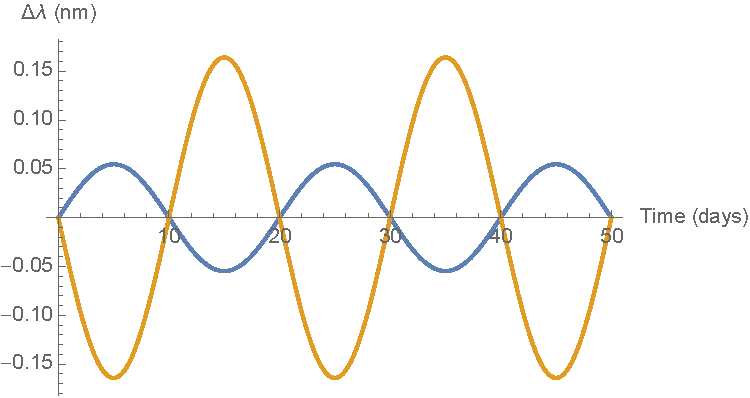
\includegraphics[width=4in]{binarycalcs/binary1.pdf}}
\index{color_page}

What's plotted on this graph are the wavelength shifts of the spectral line.
So when $t=0$ days, there is no shift at all, and both lines appear right
where they would be in the lab. A day or two later, the spectral line is split
in two, with one line (represented by the blue curve) having a wavelength slightly longer than expected, and one (represented by the yellow curve)
having a wavelength slightly shorter than expected. By 10 days, the two
spectral lines have come back together again, and then they split apart again.

As you probably know, the reason this is happening is that this star
is really a \textit{double-line spectroscopic binary system}. The two graphs
show the spectral lines due to the two stars in the system, which alternately
move toward you and away from you as they orbit around each other.

To save you the trouble of reading numbers off the graph, I'll
tell you that when $t=5$ days, the blue curve is at a height of 0.055 nm,
and the yellow curve is at $-0.16$ nm. This moment is when the two graphs
are at their highest and lowest points, meaning that one star is
moving directly toward you and one is moving directly away from you.
You can assume that the stars are moving in circular orbits.


Let's
call the star whose spectral line is given by the blue curve star number
1, and the other one star number 2. The wavelength of the H$\alpha$ line, 
when measured in the lab, is 656.3 nm. 
Armed with this information, I want you to tell me the following
about these stars and their orbits. 
(You may need some unit conversions. If so, look them up.)

\begin{enumerate}
\item How fast are the two stars moving?

\answerspace{2in}

\pagebreak[3]
\item Which star is heavier? What is the ratio of their masses $M_1/M_2$?
(Remember that the masses and speeds of the orbits are related,
so that $M_1v_1=M_2v_2$.)

\answerspace{1.5in}

\item What is the period of the orbit? (That is, how much time does
it take for the graph to repeat itself?)

\answerspace{1in}

\item What are the radii of the two stars' orbits? (Suggestion: 
How far does each star travel during one period of its motion? How
is that number related to the radius?)

\answerspace{1.5in}

\item At the end of this document is a picture of the two stars' orbits. 
You, the observer, are way off to the left. Say both stars
are moving counterclockwise.
When $t=5$ days, where are the two stars in this diagram? (Hint:
is star 1 moving toward you or away from you at this moment? What about
star 2?)
Mark the locations on the diagram with a ``5''.

\item Mark the locations of the two stars when $t=10,15$, and 20 days.
\item What is the distance between the two stars at any given time?
(Hint: How is it related to the radii of the two orbits, which you know?)
The distance between the two stars is the $a$ in Kepler's Third Law.

\answerspace{1in}

\item What is the total mass $M_1+M_2$?

\answerspace{1in}
\item What are the masses $M_1$ and $M_2$?
\end{enumerate}

\centerline{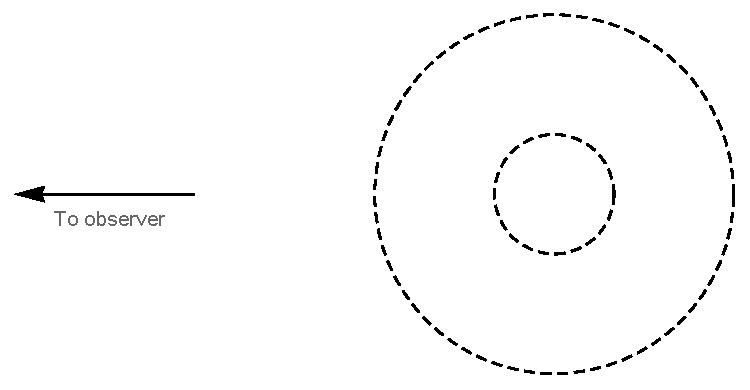
\includegraphics[width=4in]{binarycalcs/binary2.pdf}}

%% \vfil

%% {\bf Answers} (without all the detailed steps, and skipping the ones whose 
%% answers are pictures, because I'm lazy):

%% 1. $v_1=\SI{25000}{m/s}$, $v_2 = \SI{73000}{m/s}$.

%% 2. $M_1/M_2 = 2.9$.

%% 3. 20 days.

%% 4. $r_1=\SI{6.8e9}{m}$, $r_2 = \SI{2.0e10}{m}$.

%% 7. \SI{2.7e10}{m}.

%% 8. $1.95M_\odot$.

%% 9. $M_1 = 1.45M_\odot, M_1=0.5M_\odot$.



\section{Planetary Nebulae}

\makelabheader

This lab is available at http://web.williams.edu/astronomy/research/PN/nebulae/exercise1.php.

\bigskip\bigskip

\bigskip\bigskip

\bigskip\bigskip

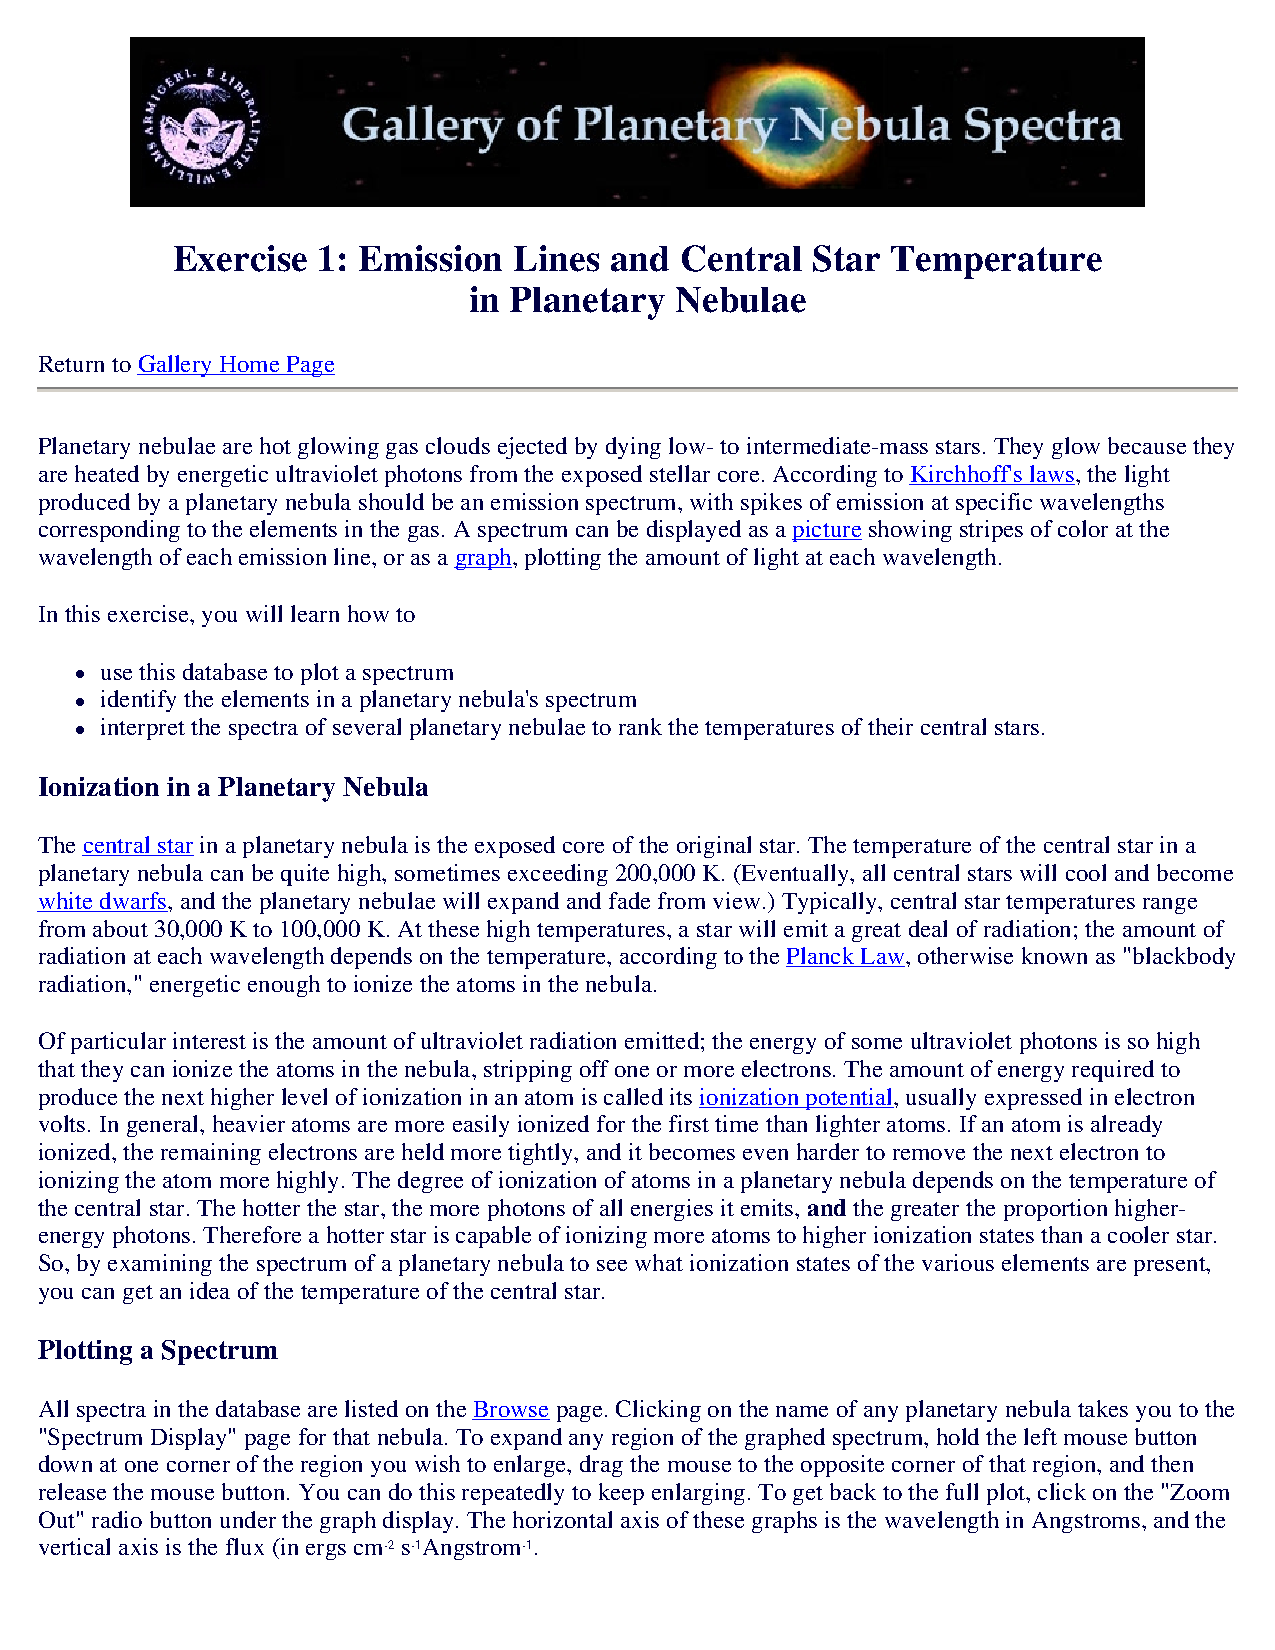
\includegraphics[height=7in,trim=-0.5in -0.6in 0 1.6in]{pna/pna1.pdf}
\newpage

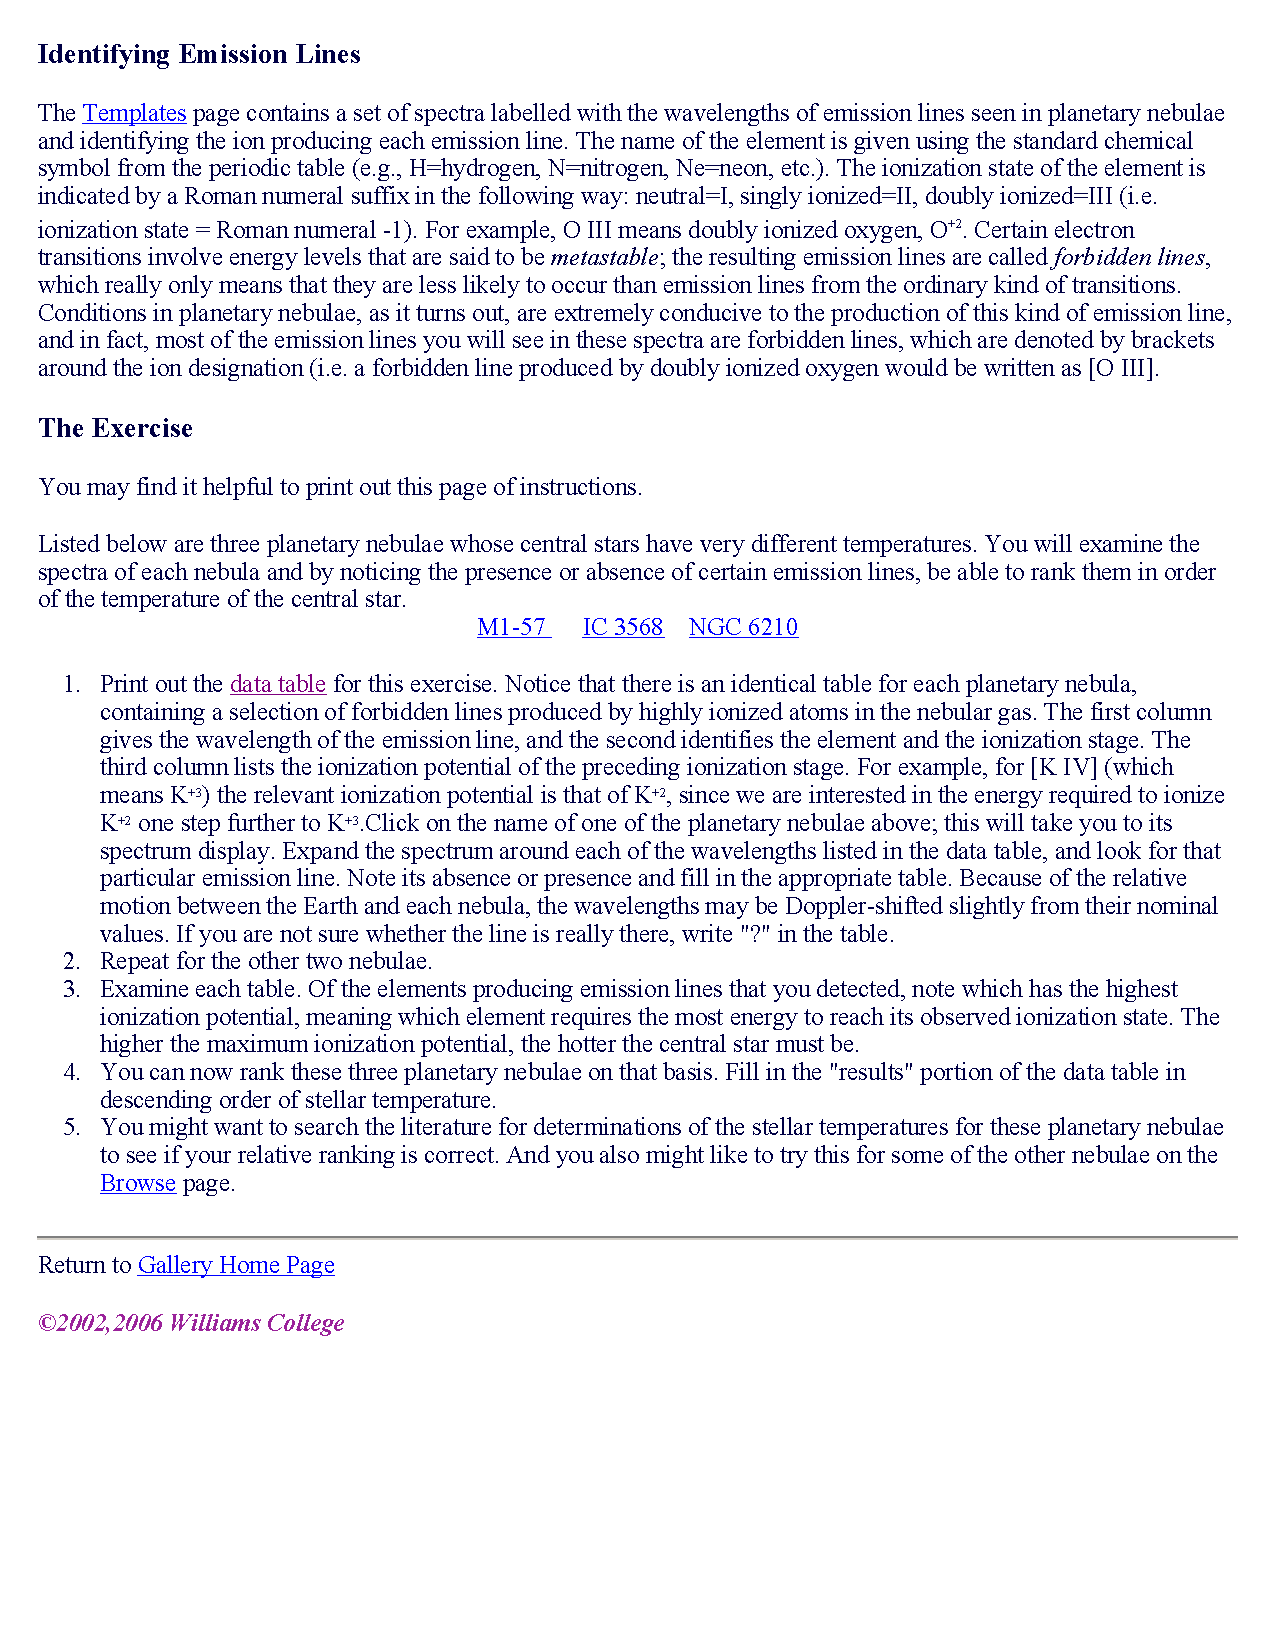
\includegraphics[height=8in]{pna/pna2.pdf}
\newpage

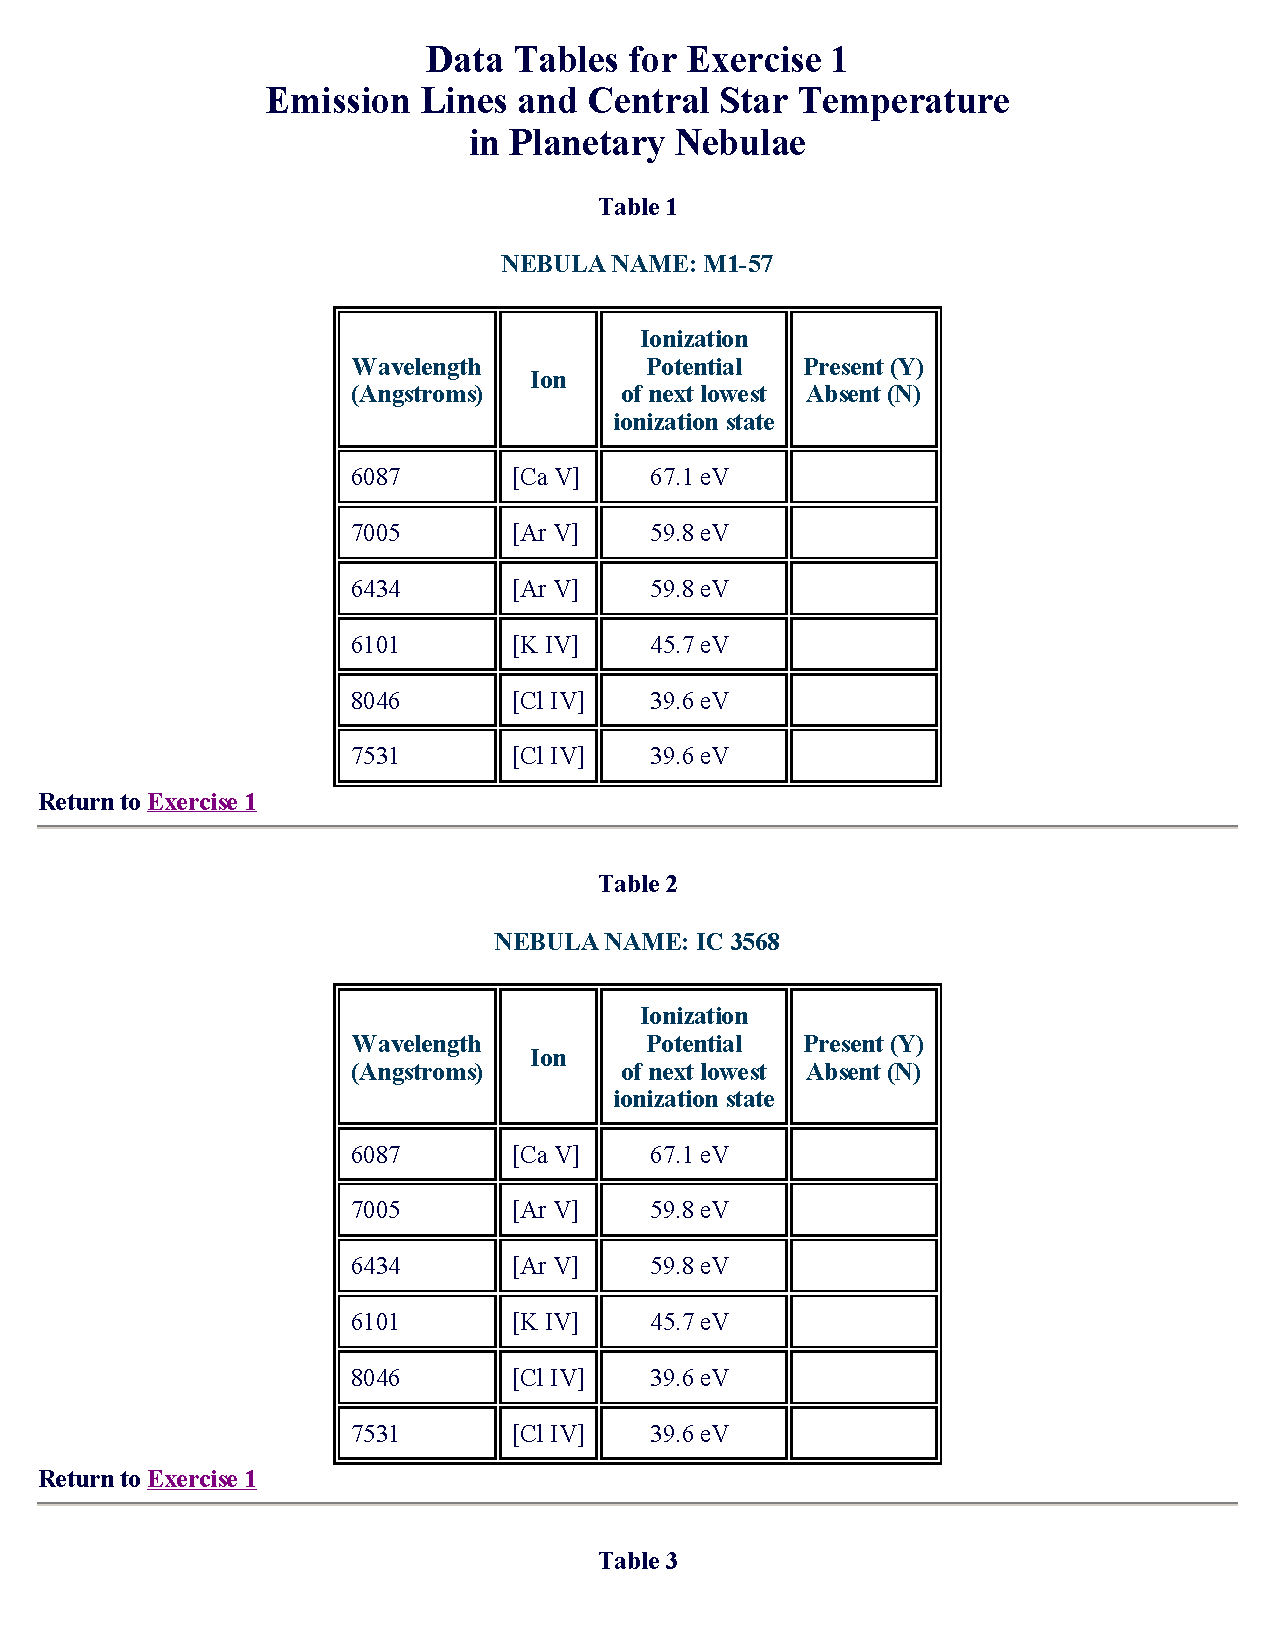
\includegraphics[height=8in]{pna/pna3.pdf}
\newpage
%\vfil\eject

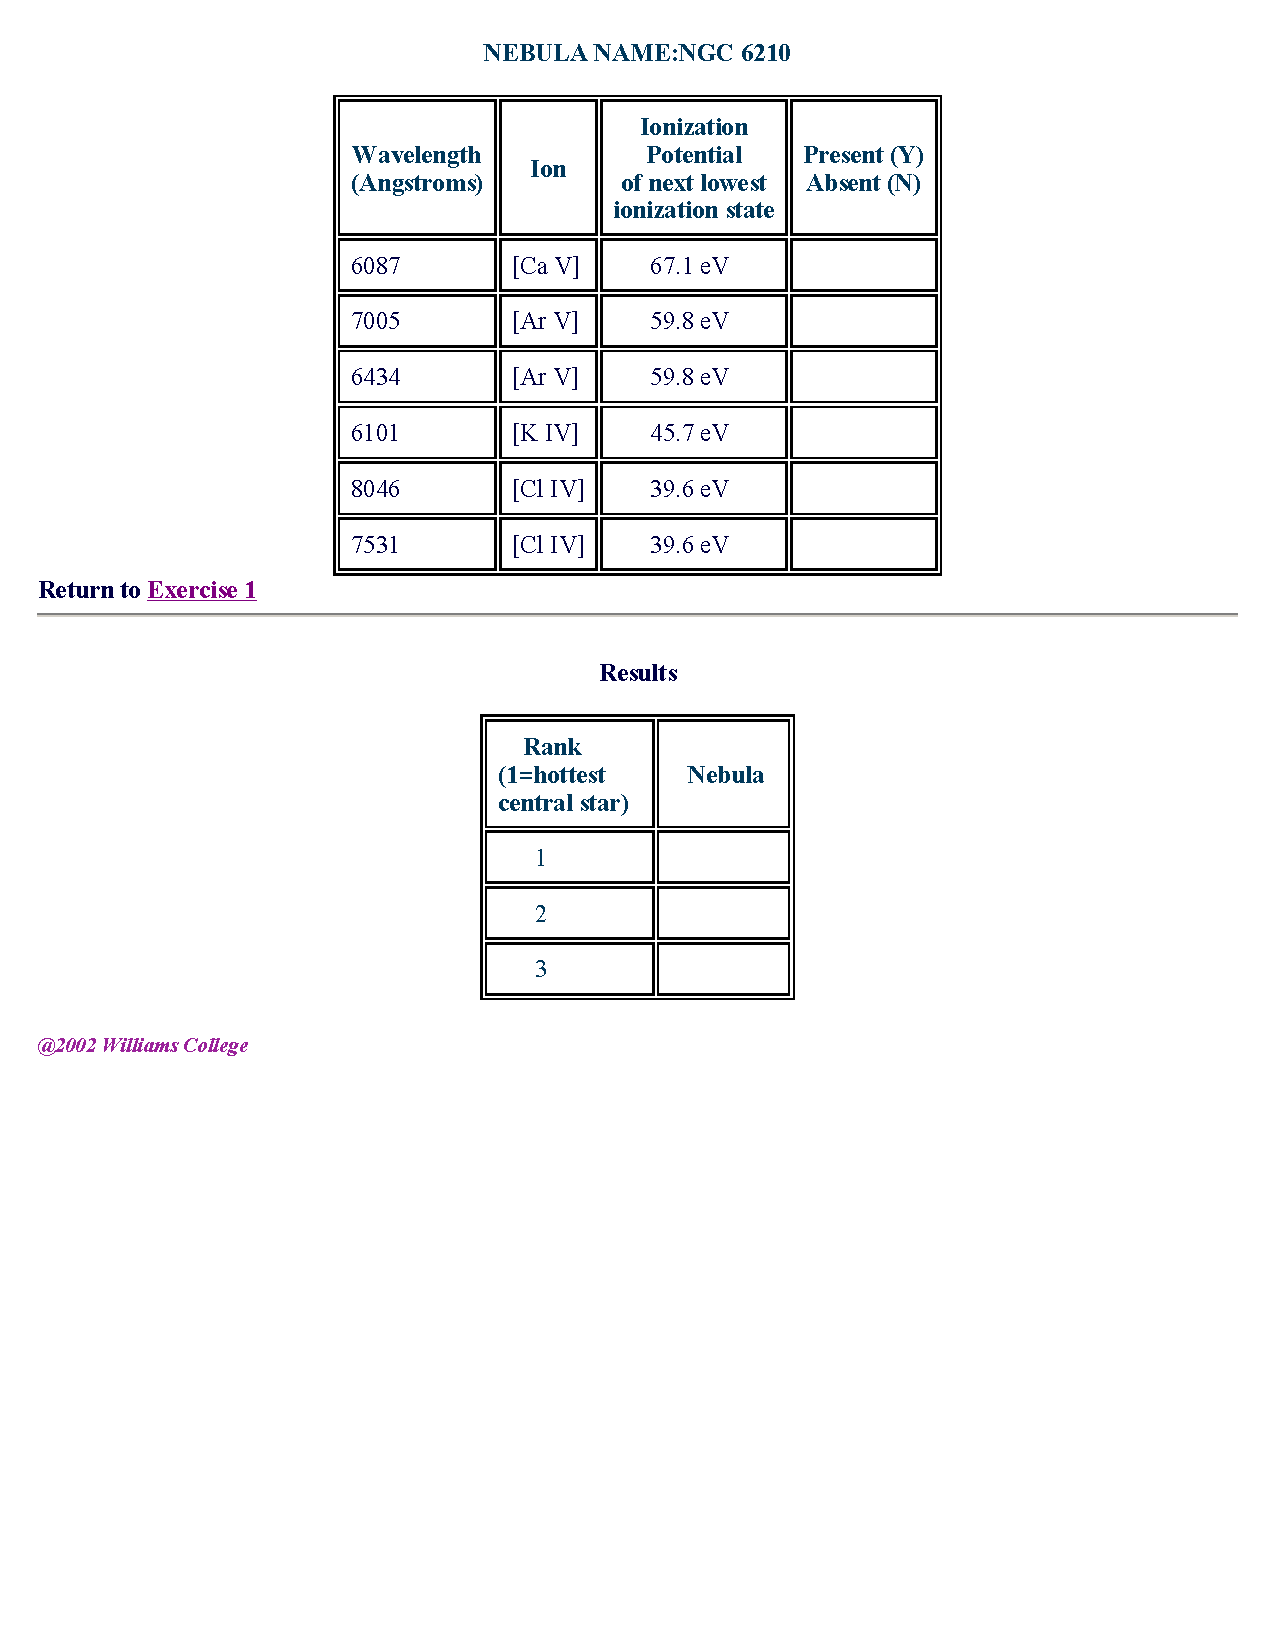
\includegraphics[height=8in]{pna/pna4.pdf}
\newpage
%\vfil\eject

\chapter{Planetary Nebulae 2}

This lab is available at http://web.williams.edu/astronomy/research/PN/nebulae/exercise2.php .

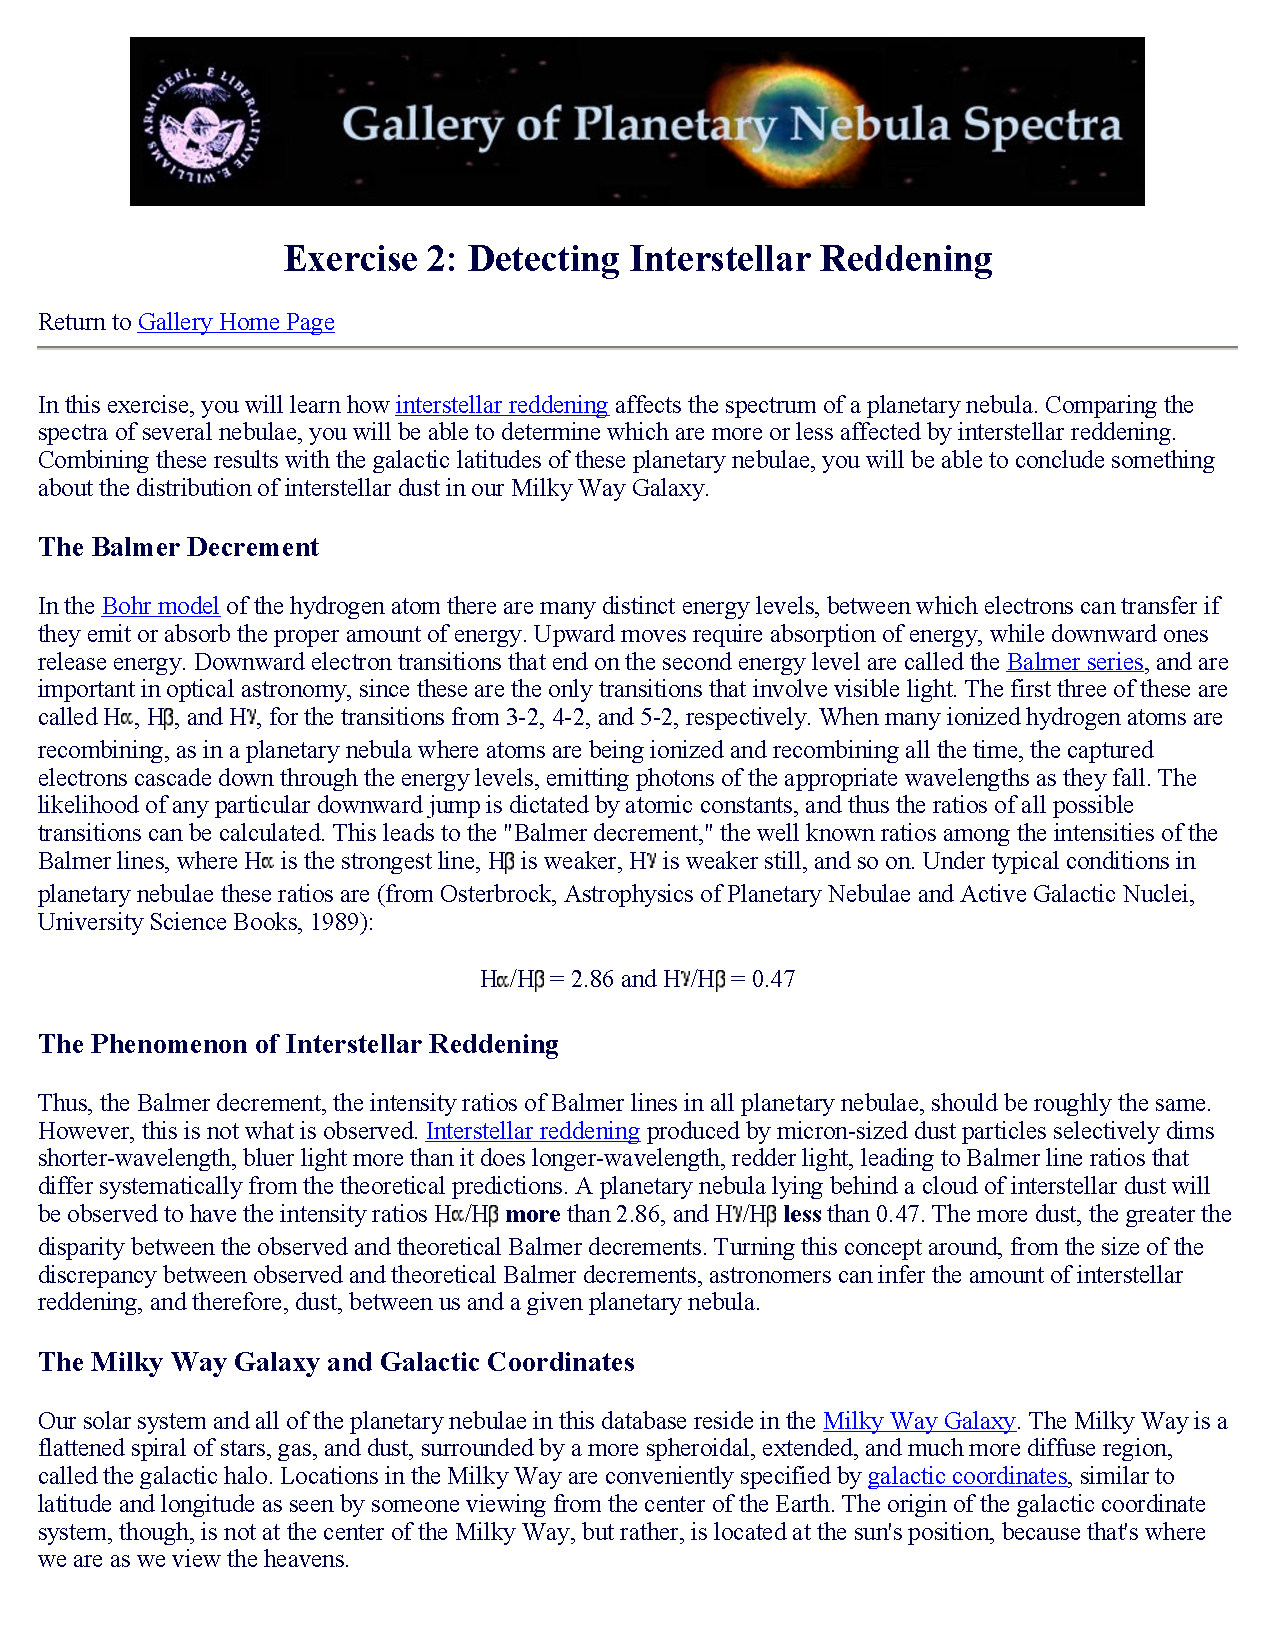
\includegraphics[height=6in]{planetary/pnb1.epsi}

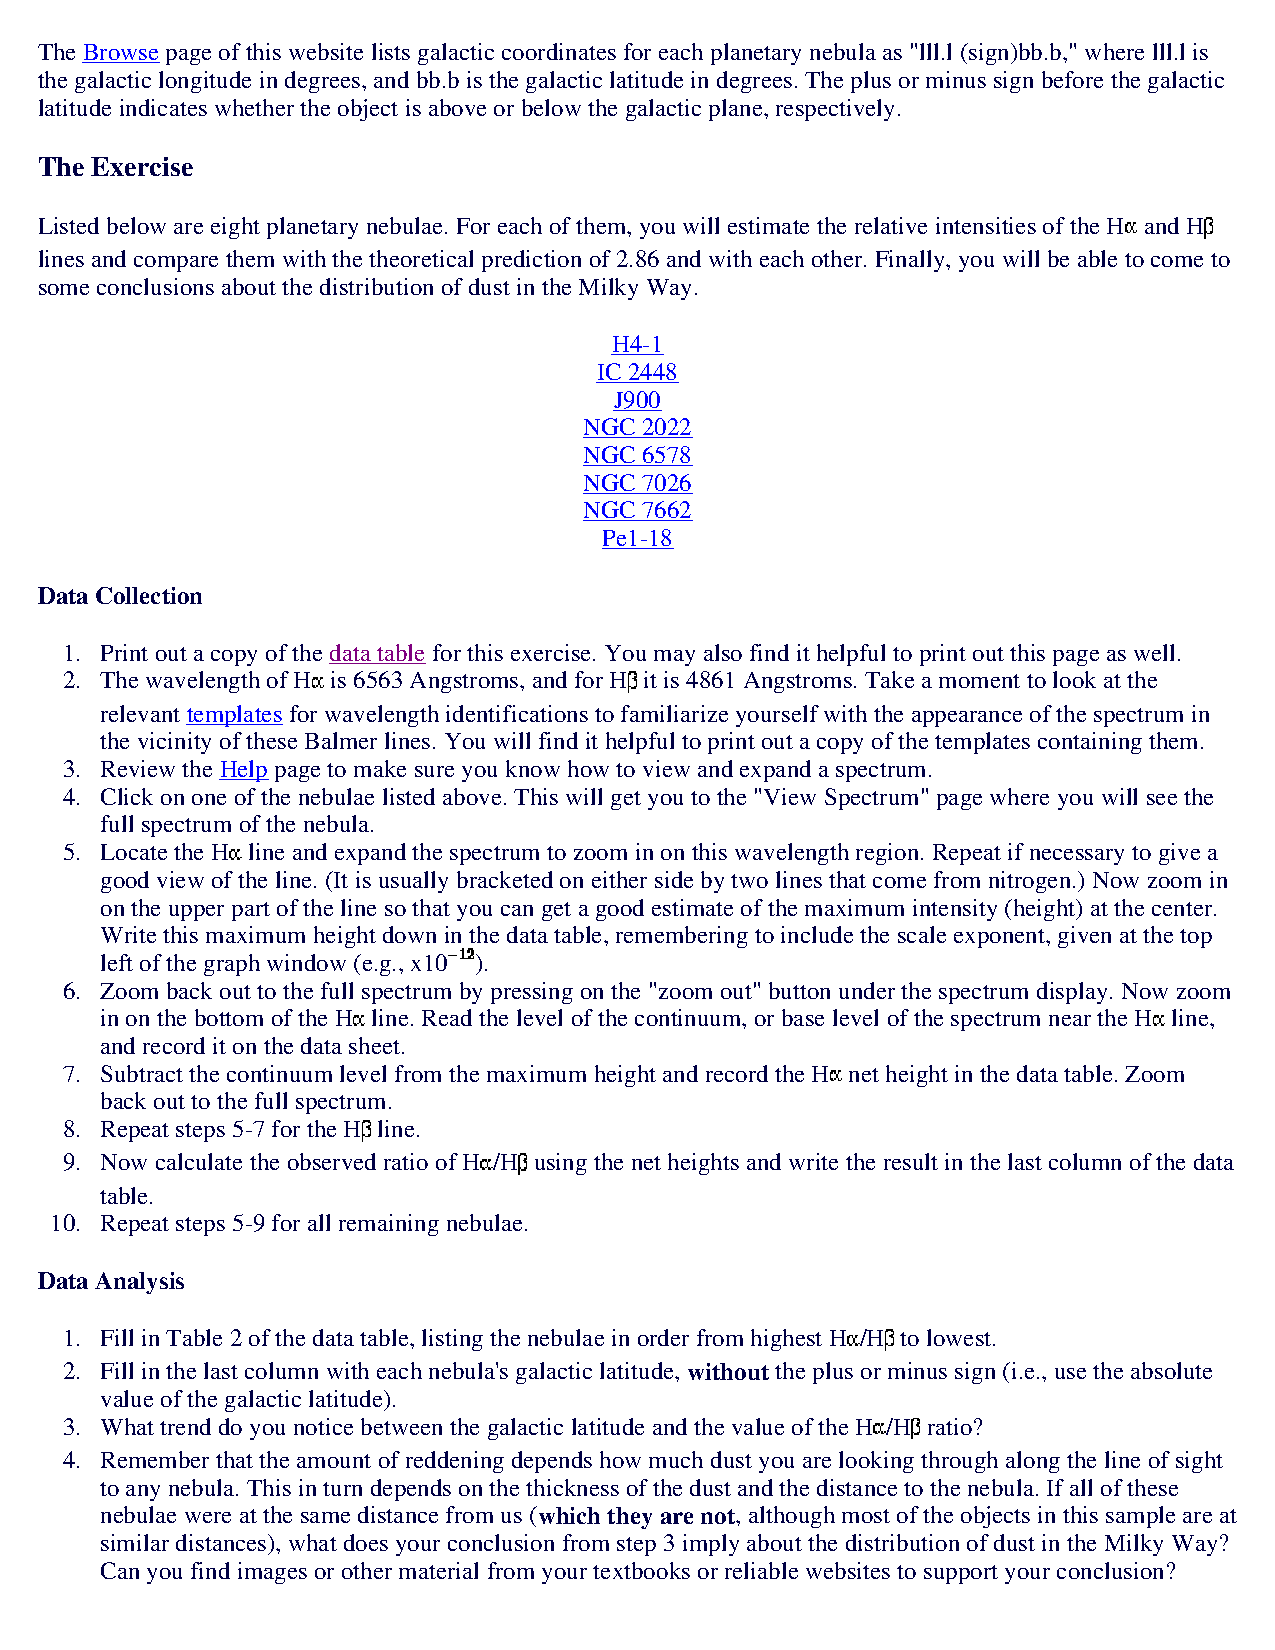
\includegraphics[height=8in]{planetary/pnb2.epsi}

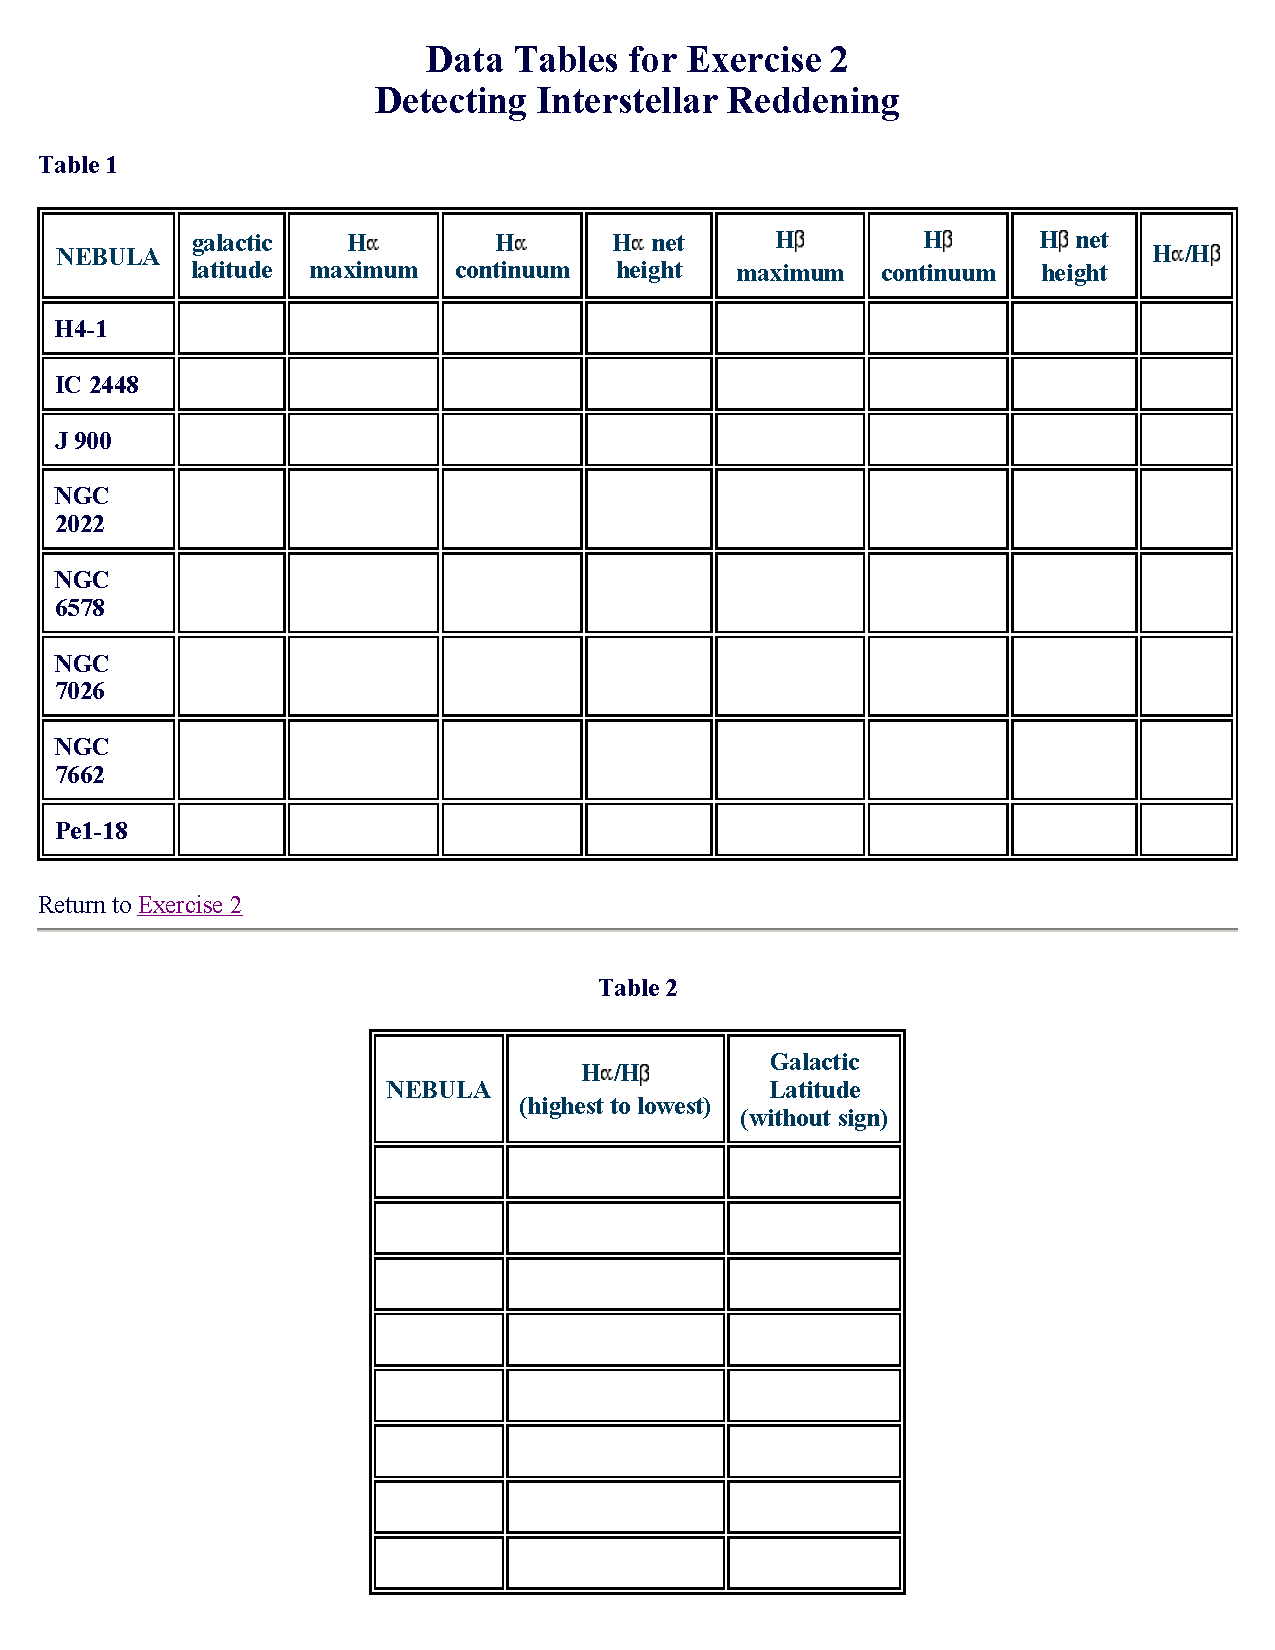
\includegraphics[height=7in]{planetary/pnb4.epsi}


\section{Radio Astronomy of Pulsars}

\makelabheader

\bigskip\bigskip

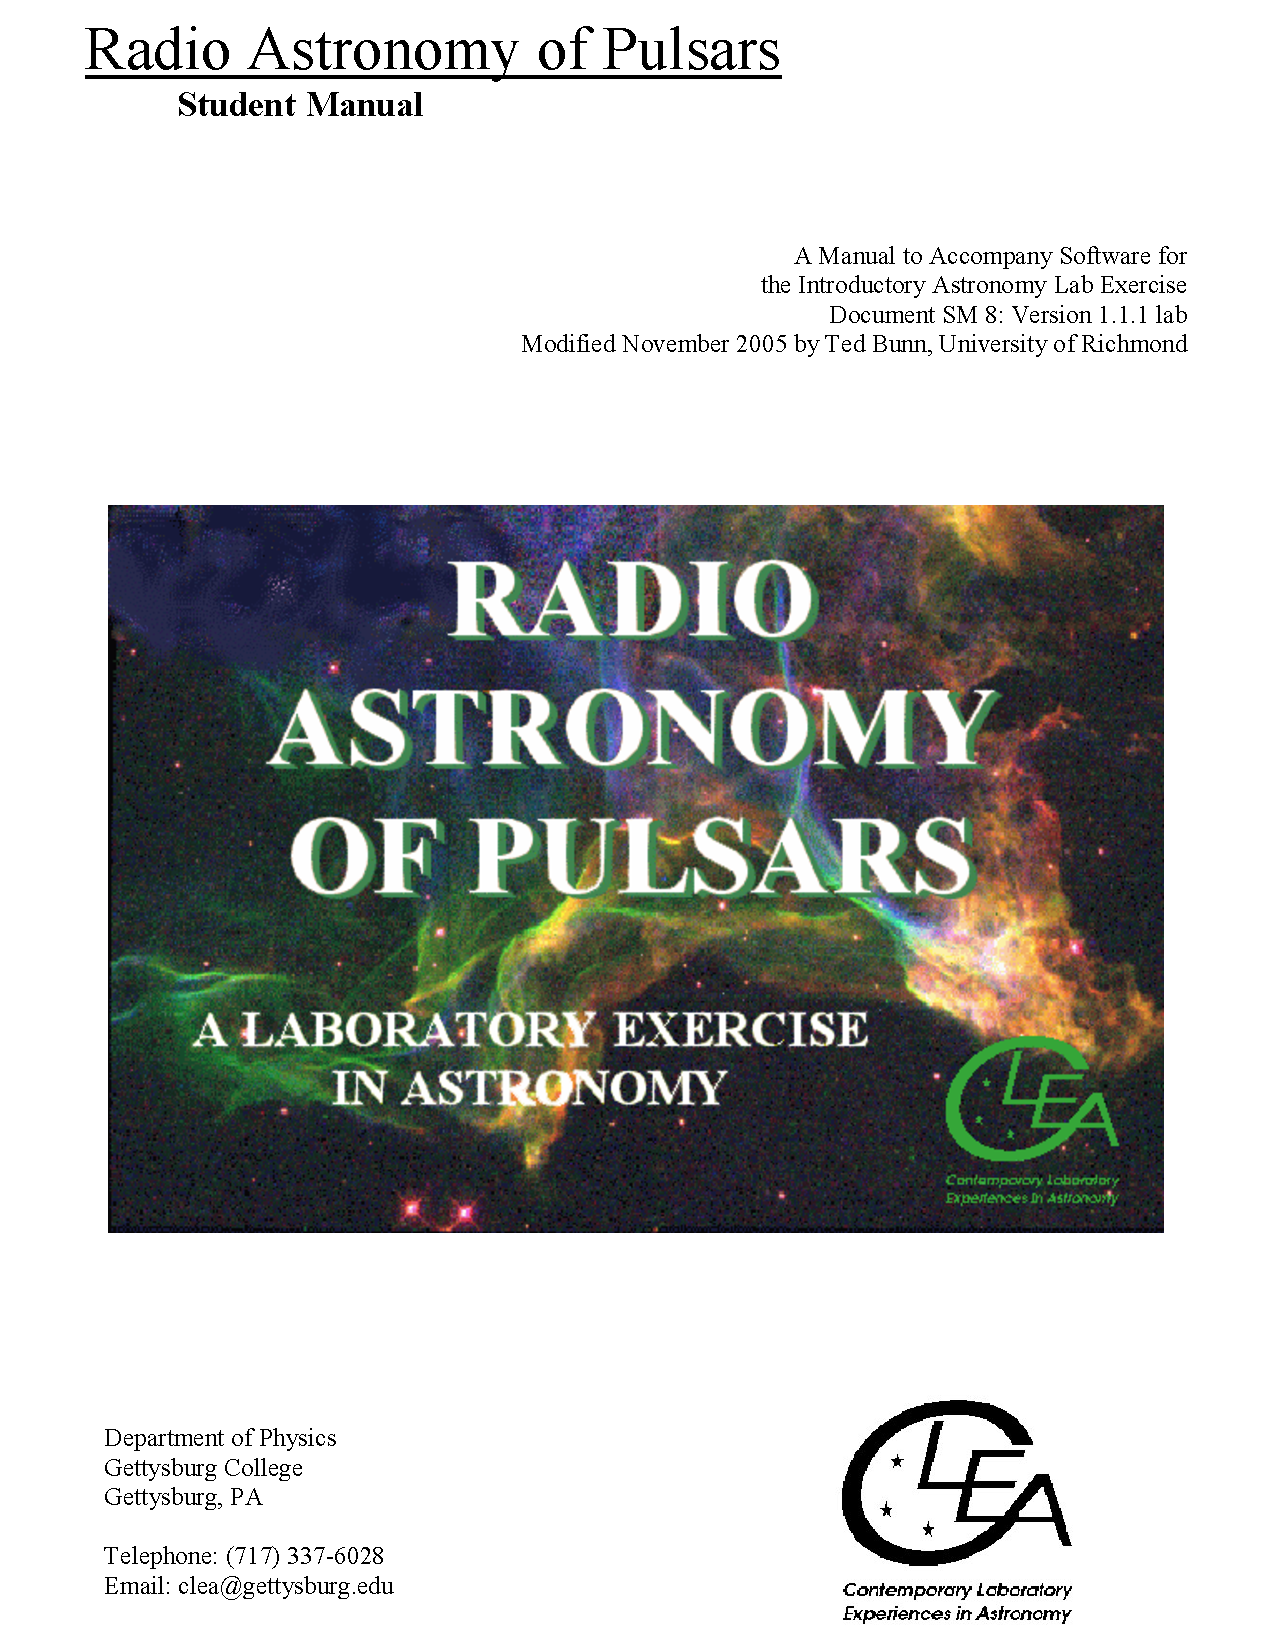
\includegraphics[height=8in]{pulsars/pulsar1.pdf}
\vfil\eject

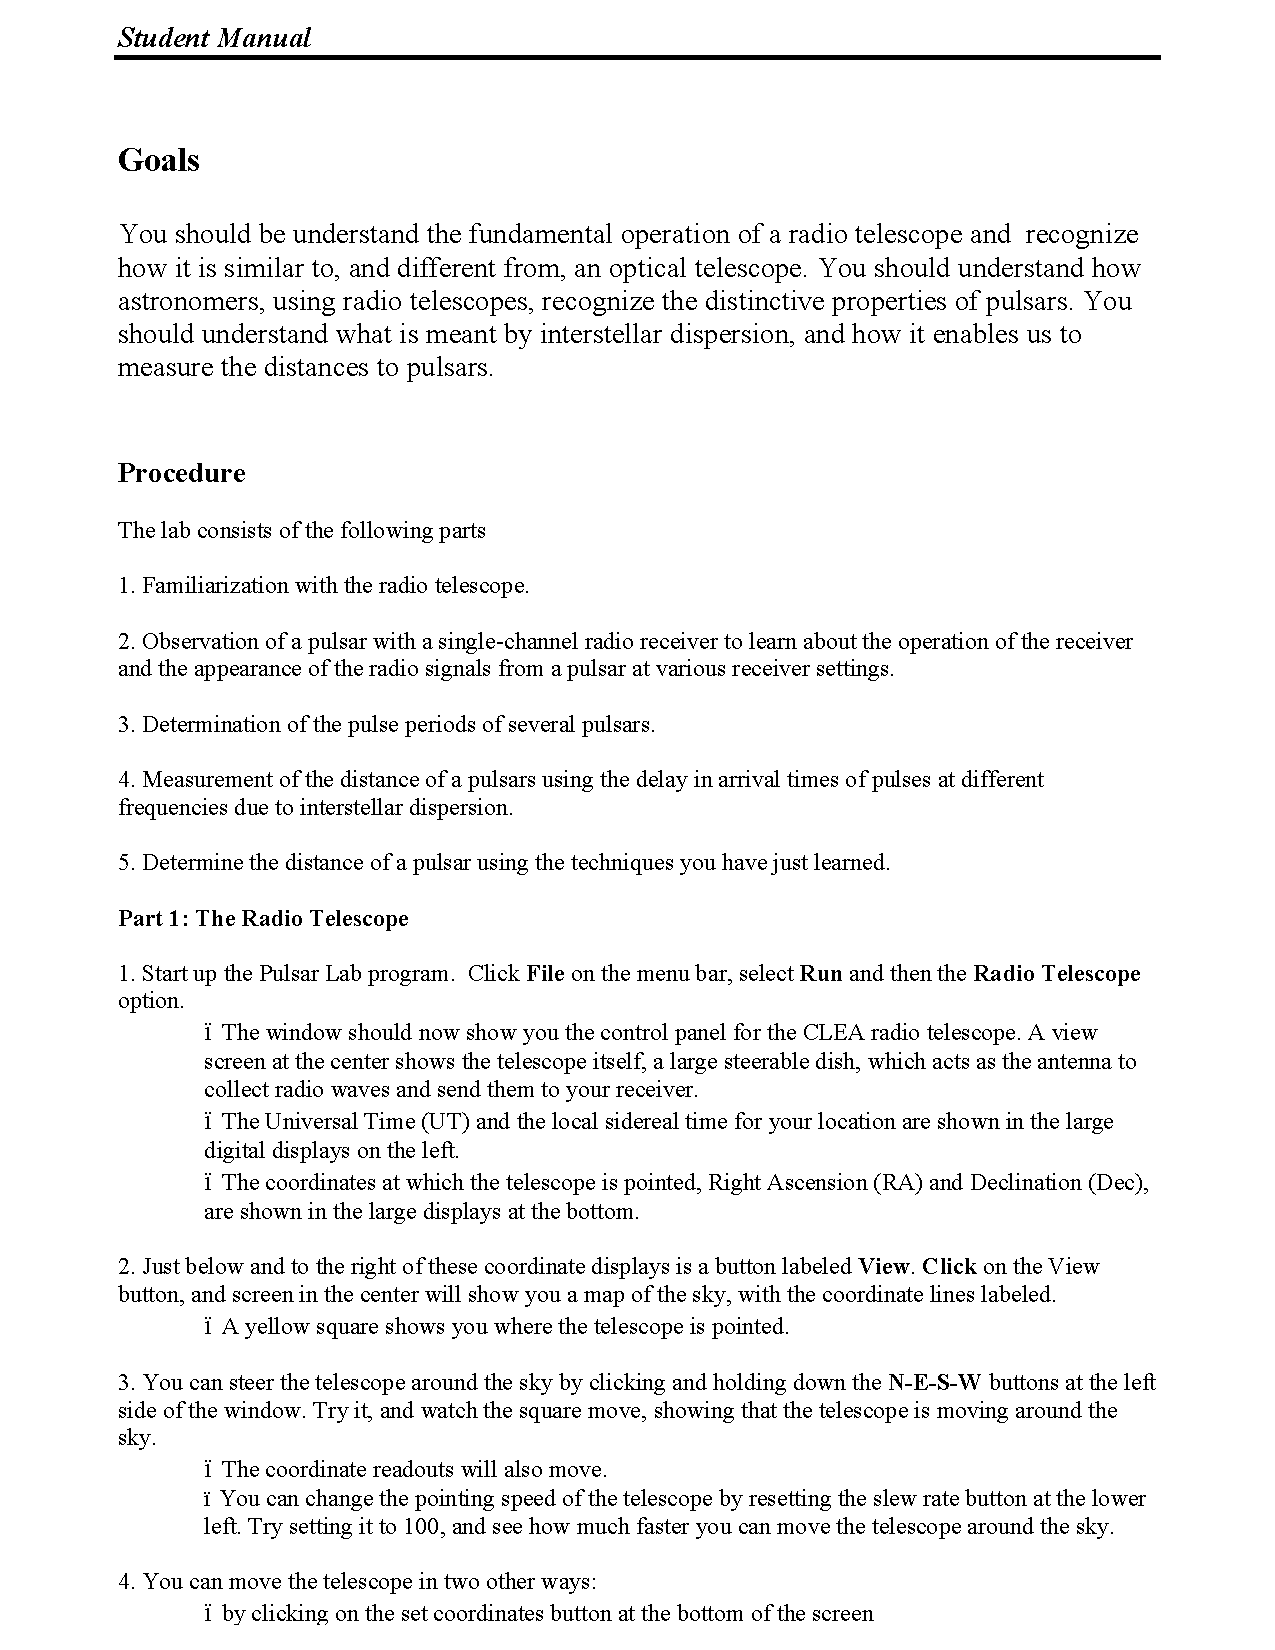
\includegraphics[width=\textwidth]{pulsars/pulsar2.pdf}
\vfil\eject

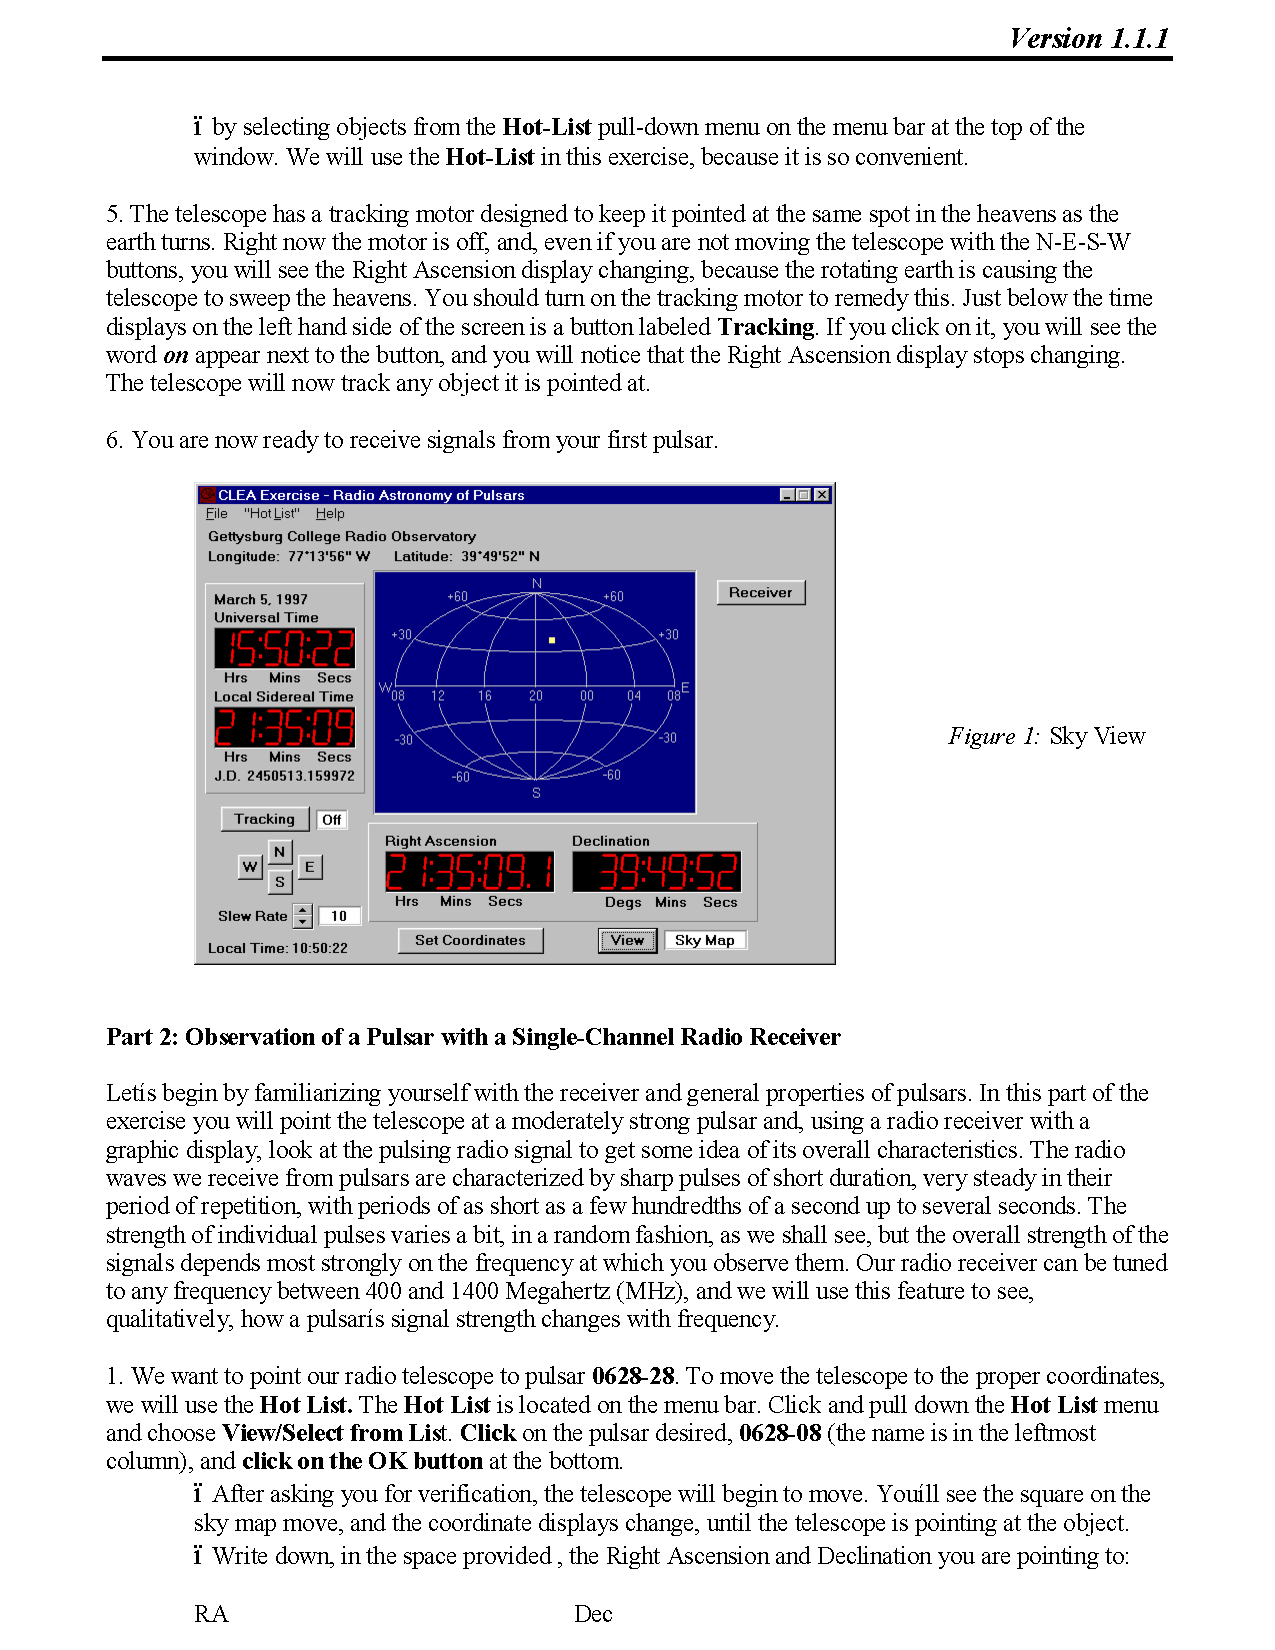
\includegraphics[width=\textwidth]{pulsars/pulsar3.pdf}
\vfil\eject

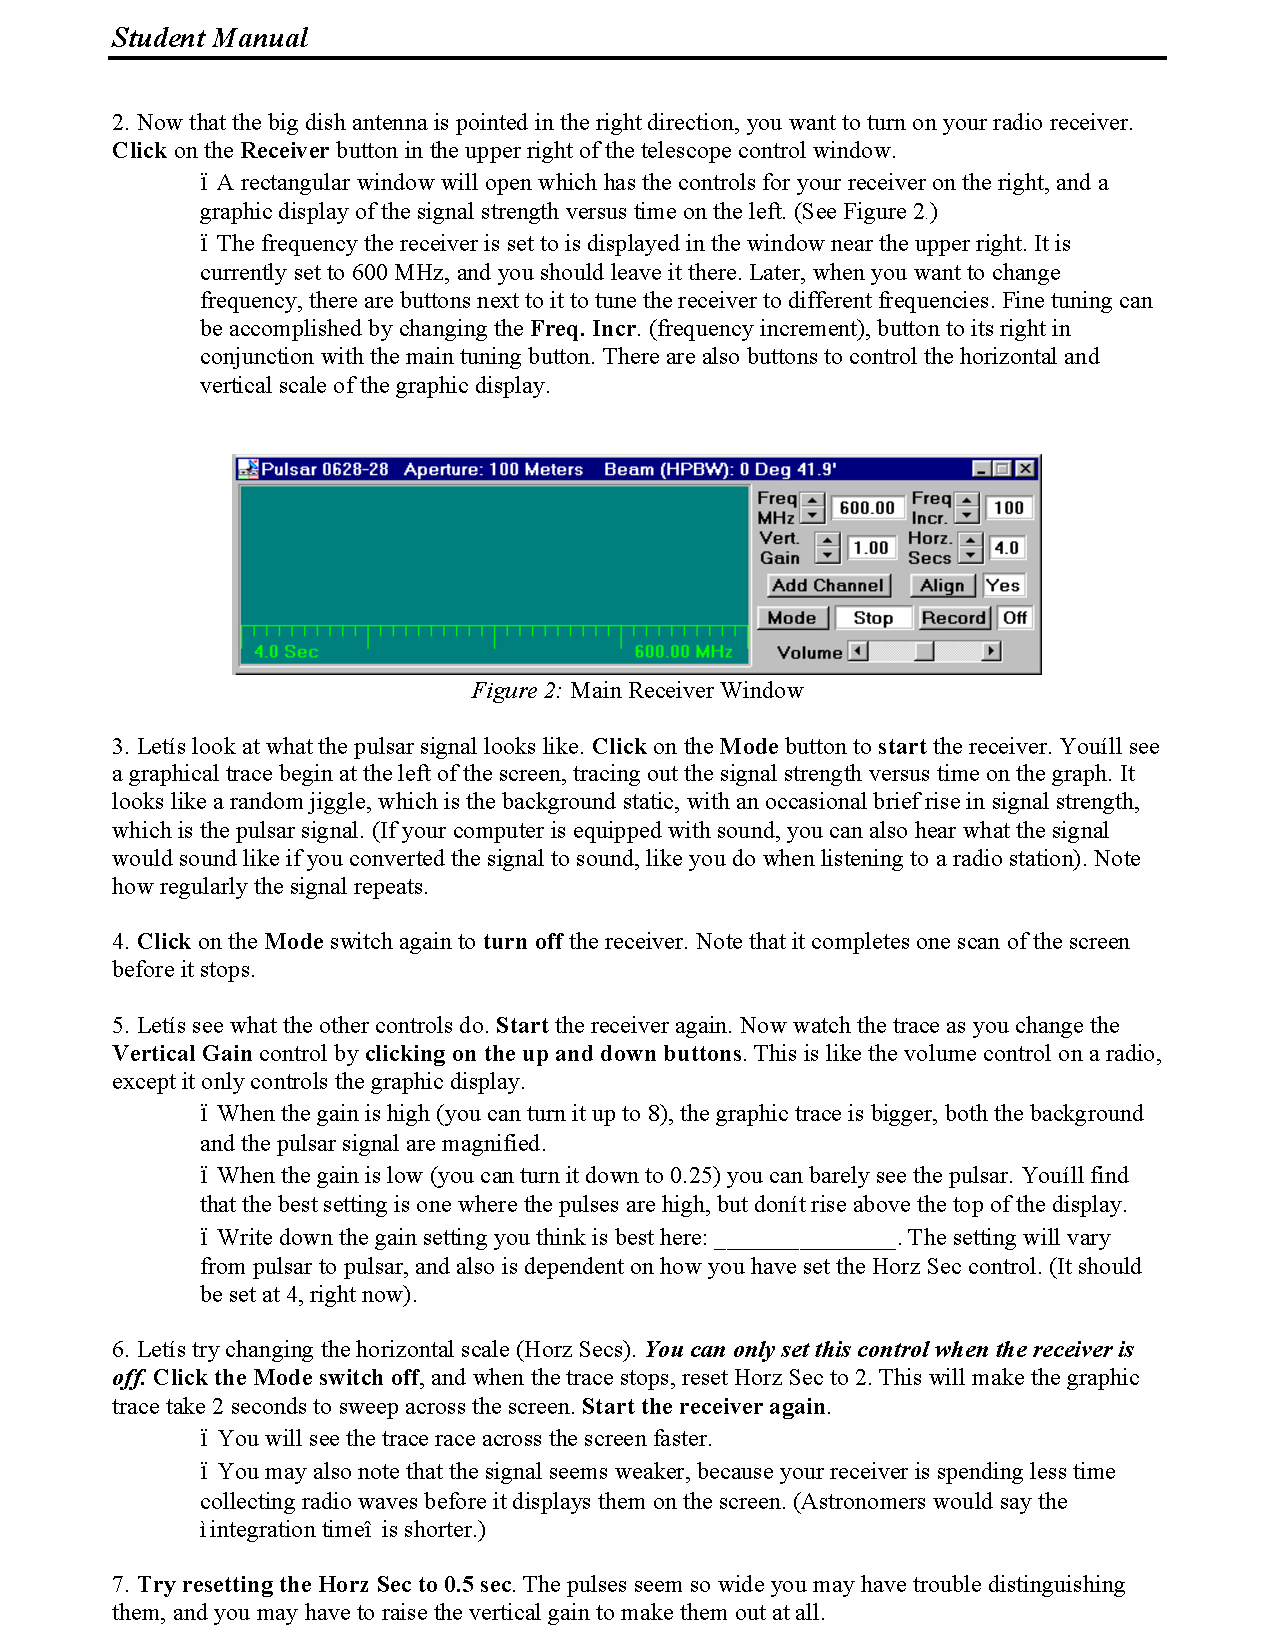
\includegraphics[width=\textwidth]{pulsars/pulsar4.pdf}
\vfil\eject

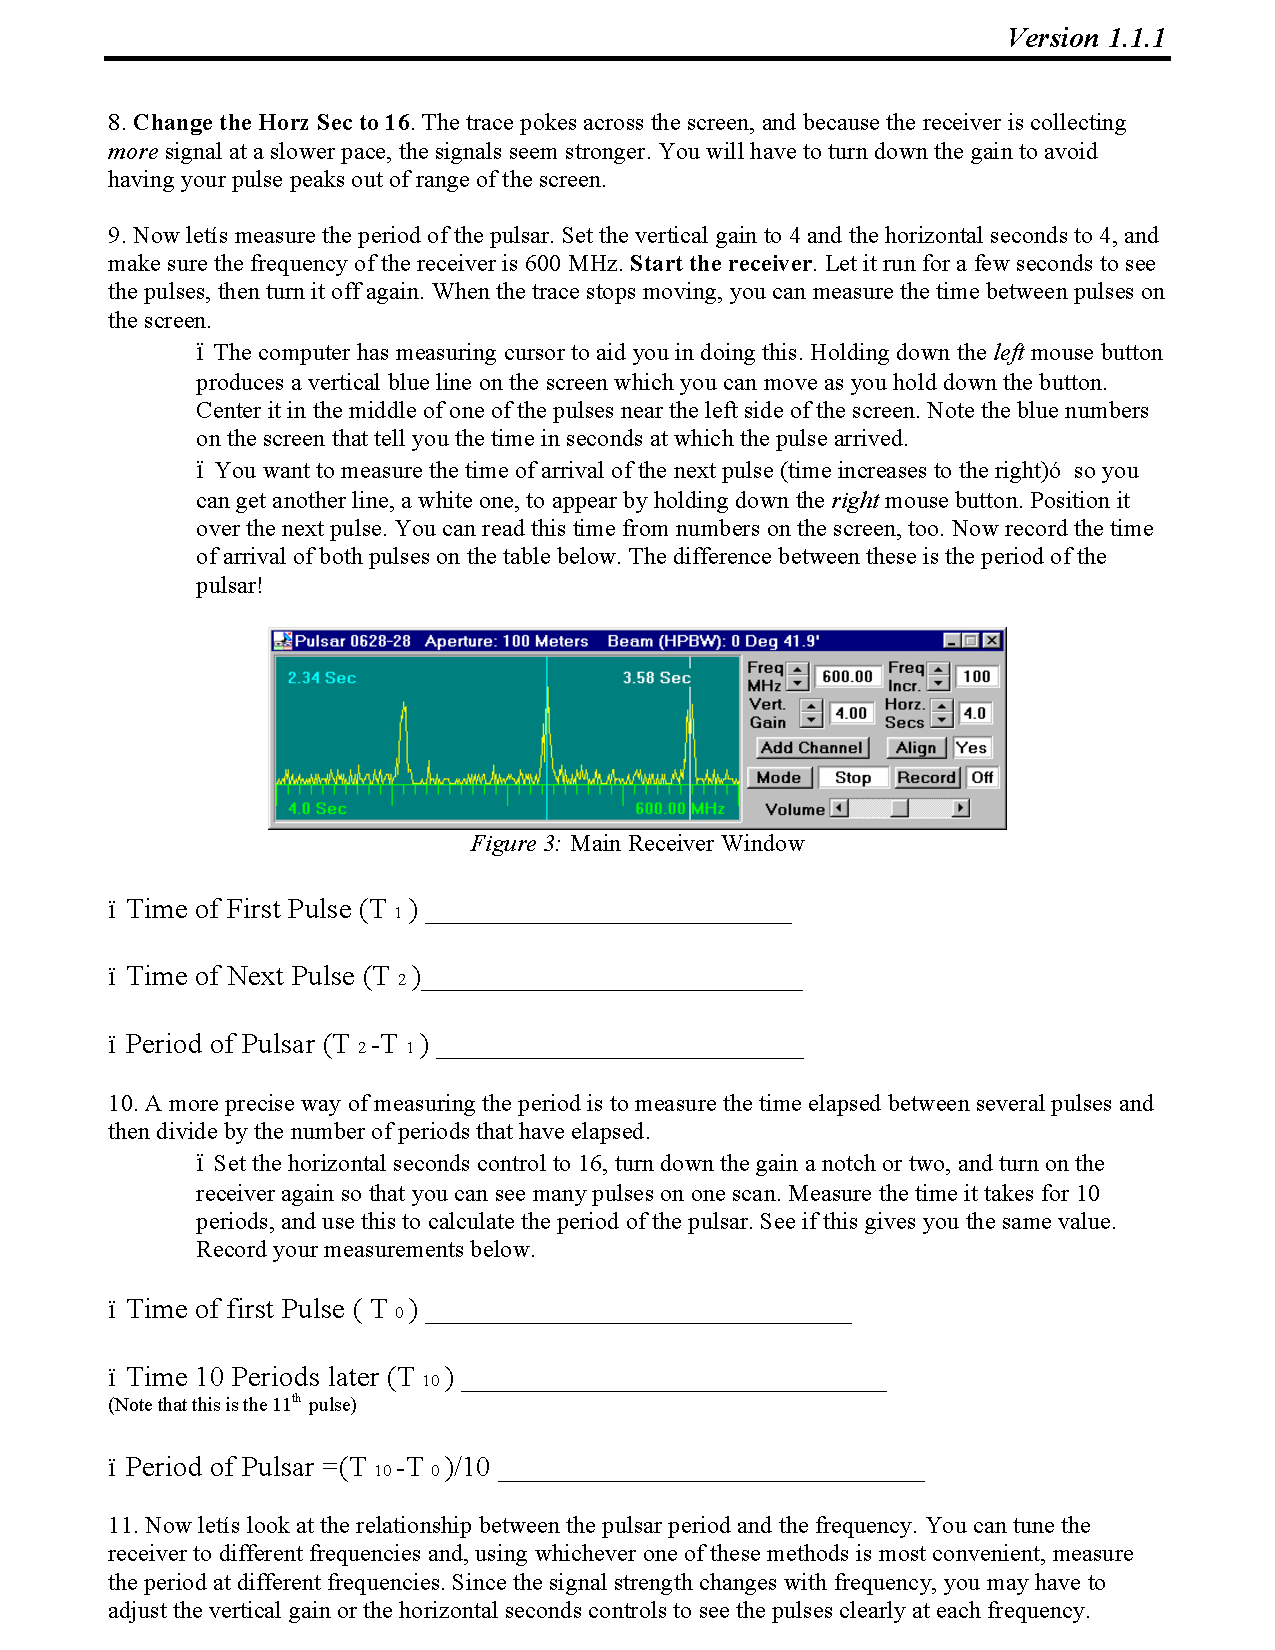
\includegraphics[width=\textwidth]{pulsars/pulsar5.pdf}
\vfil\eject

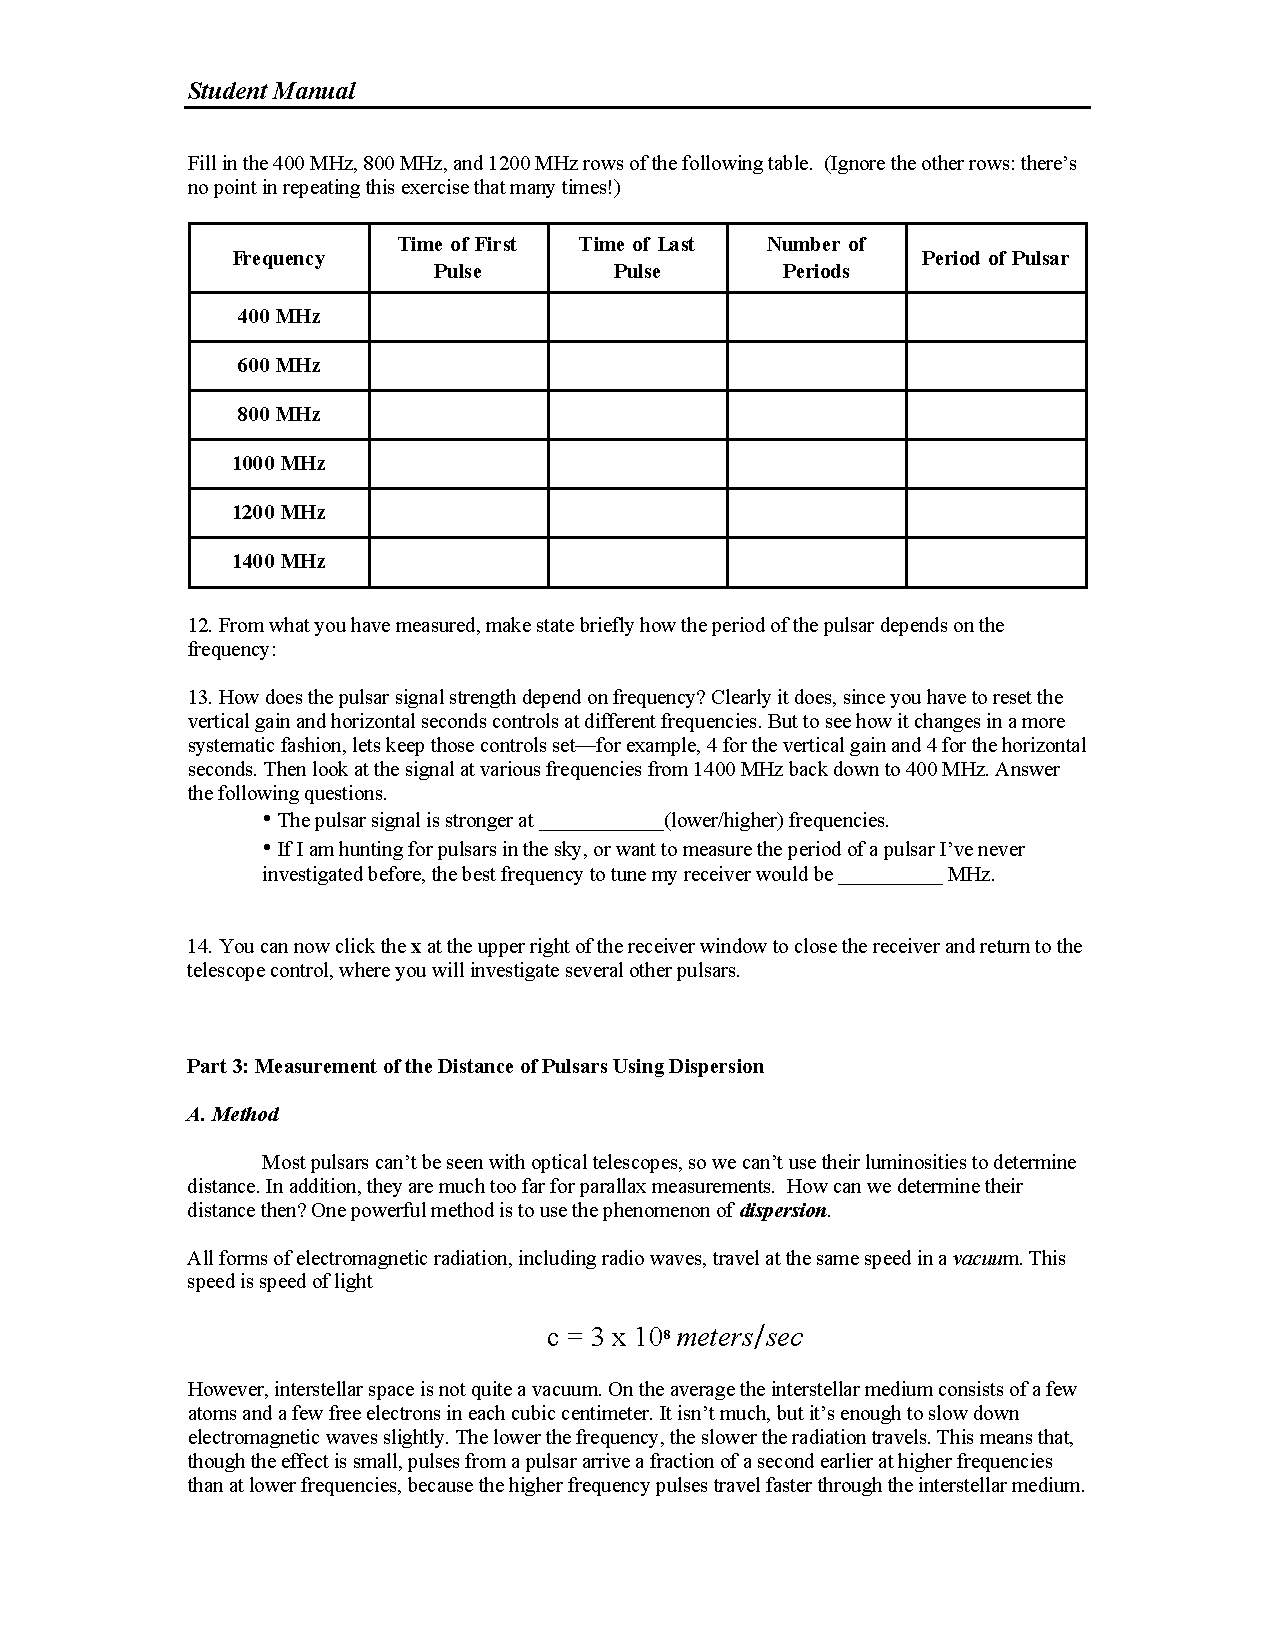
\includegraphics[width=\textwidth]{pulsars/pulsar6.pdf}
\vfil\eject

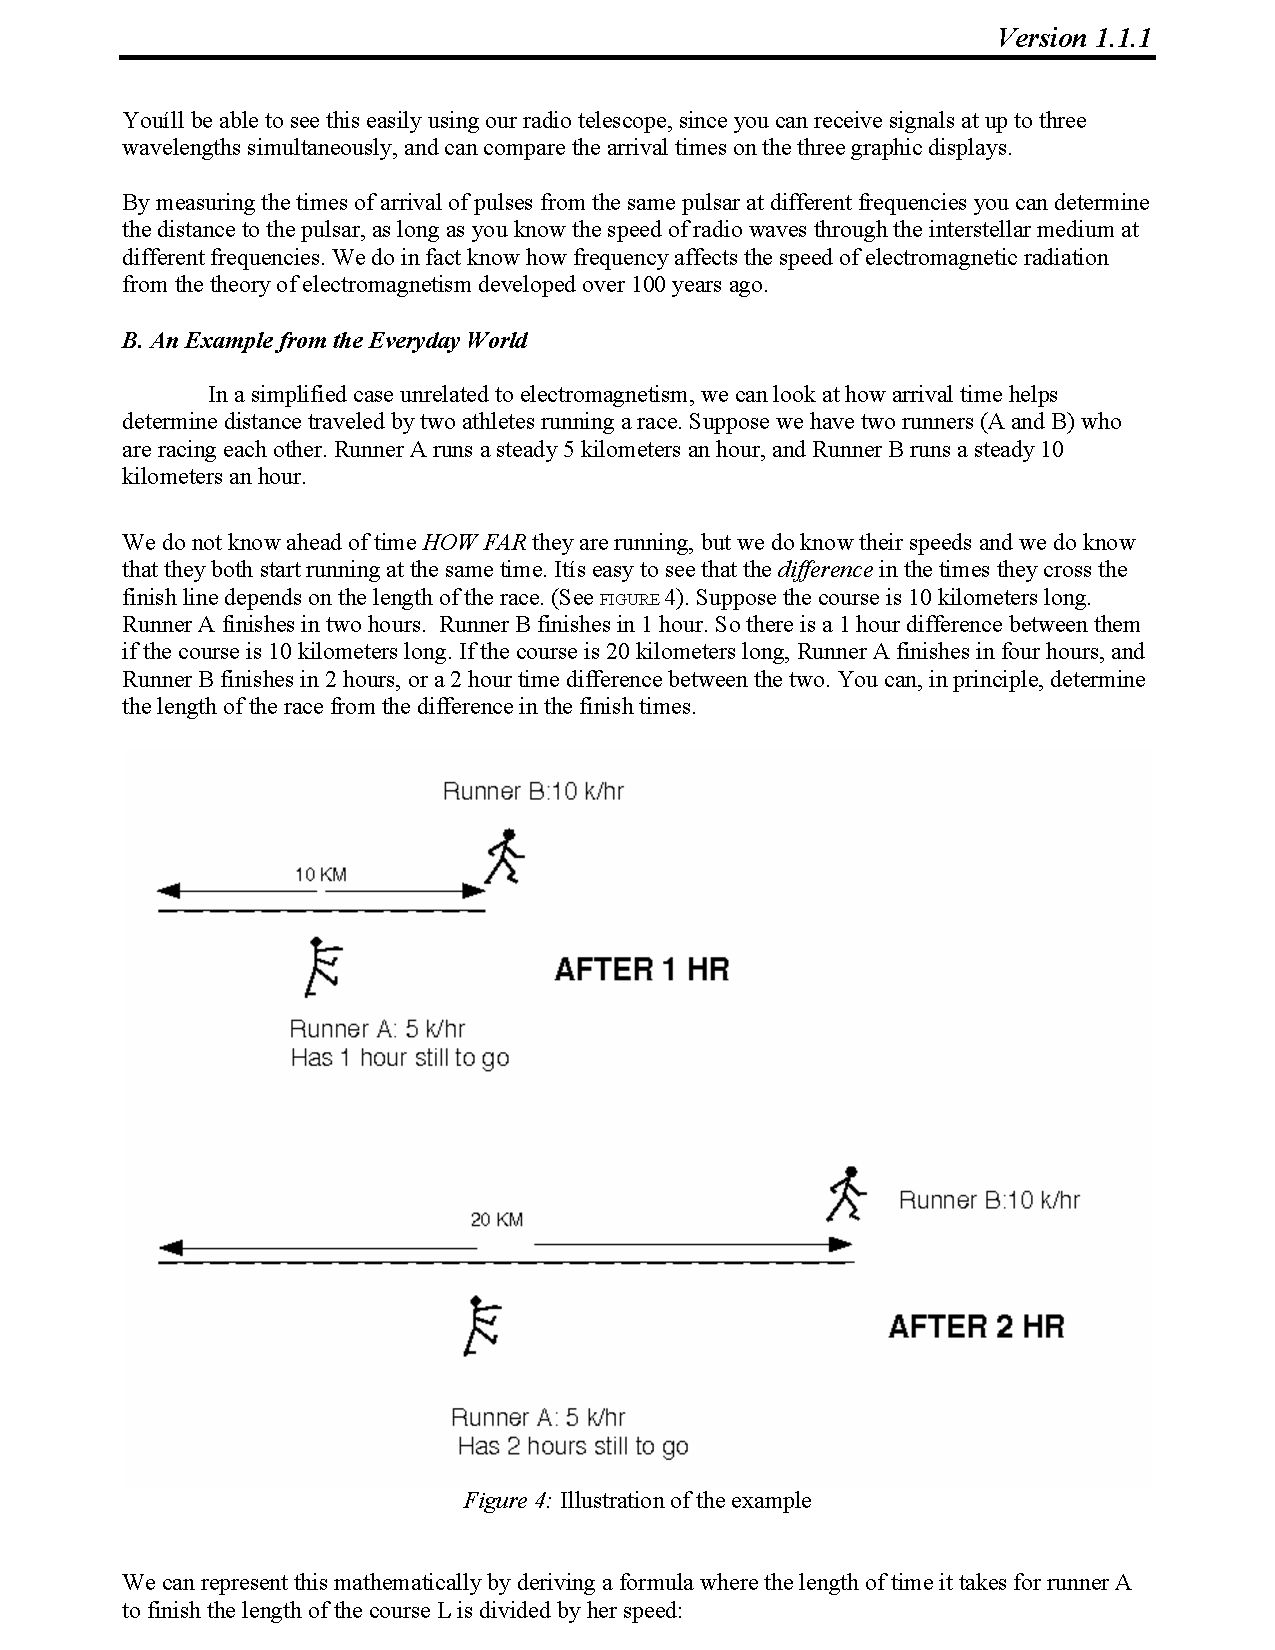
\includegraphics[width=\textwidth]{pulsars/pulsar7.pdf}
\vfil\eject

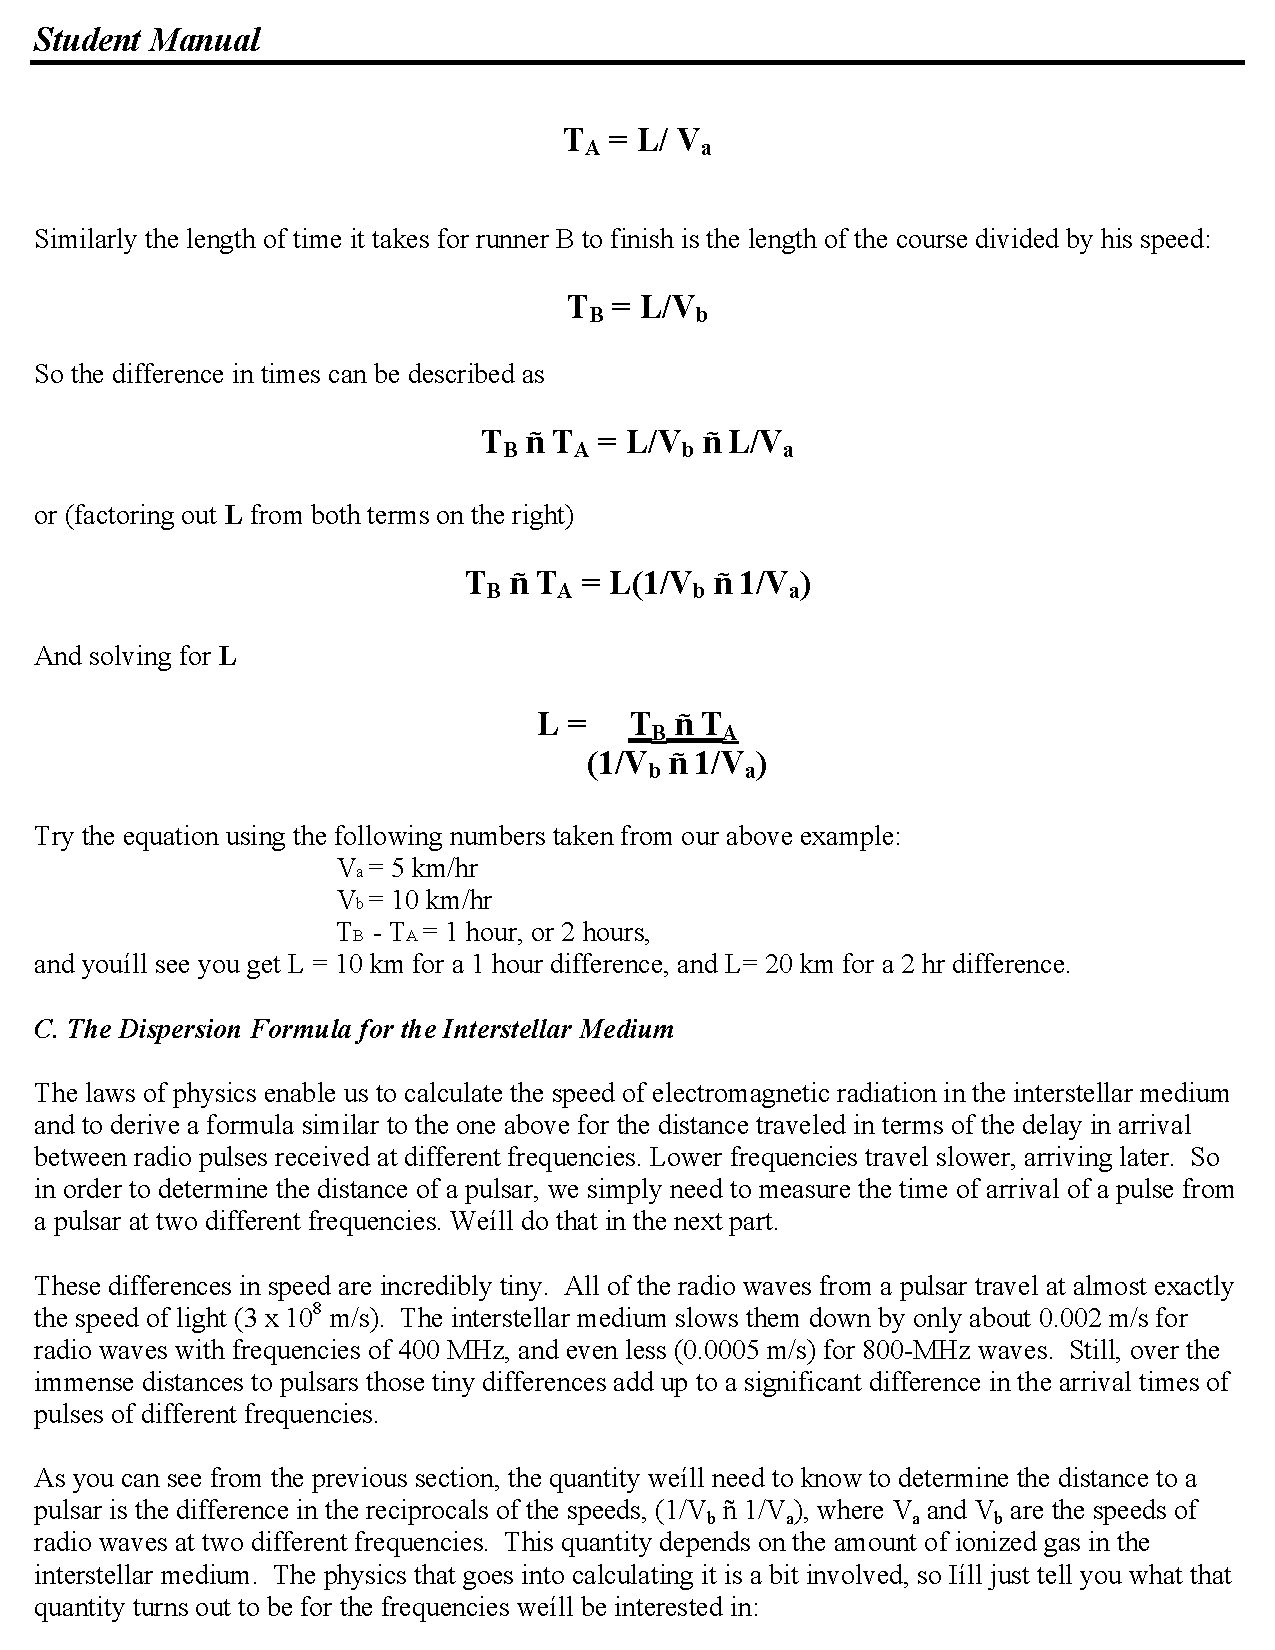
\includegraphics[width=\textwidth]{pulsars/pulsar8.pdf}
\vfil\eject

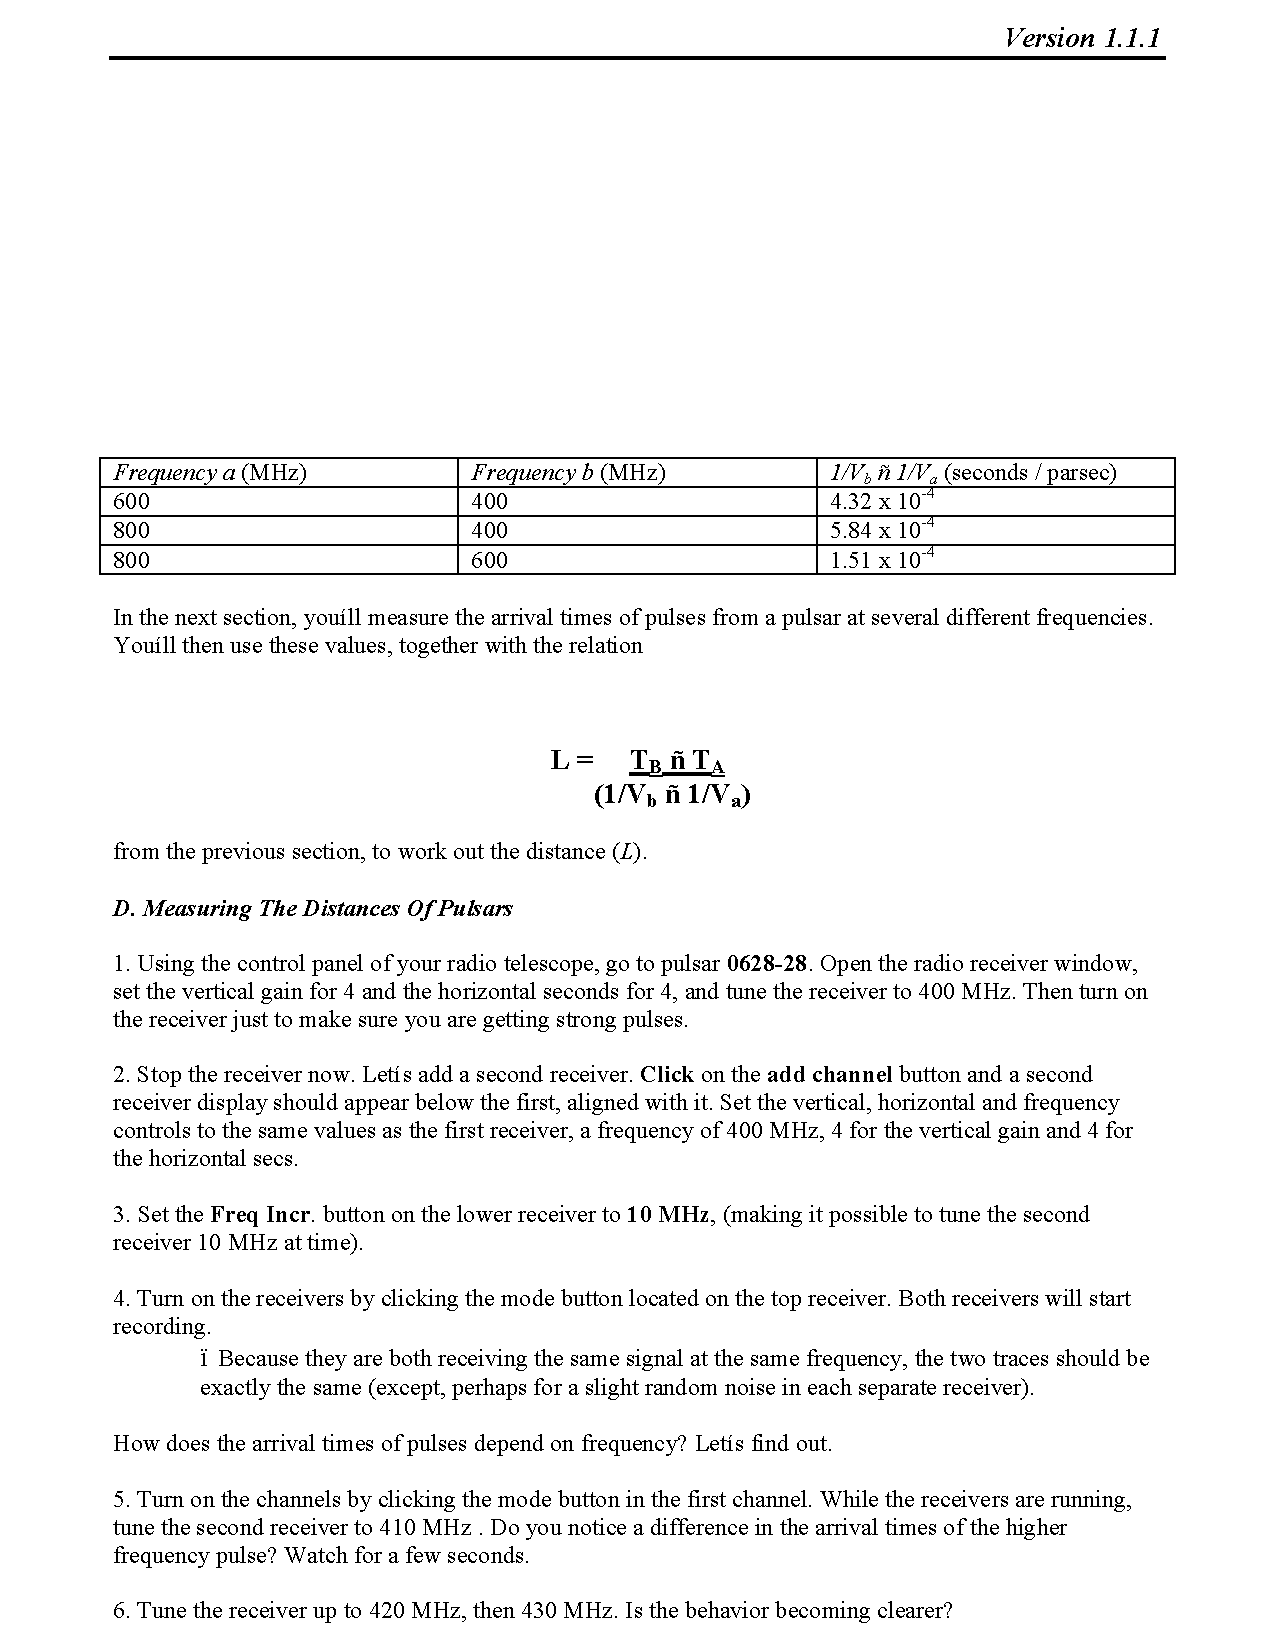
\includegraphics[width=\textwidth]{pulsars/pulsar9.pdf}
\vfil\eject

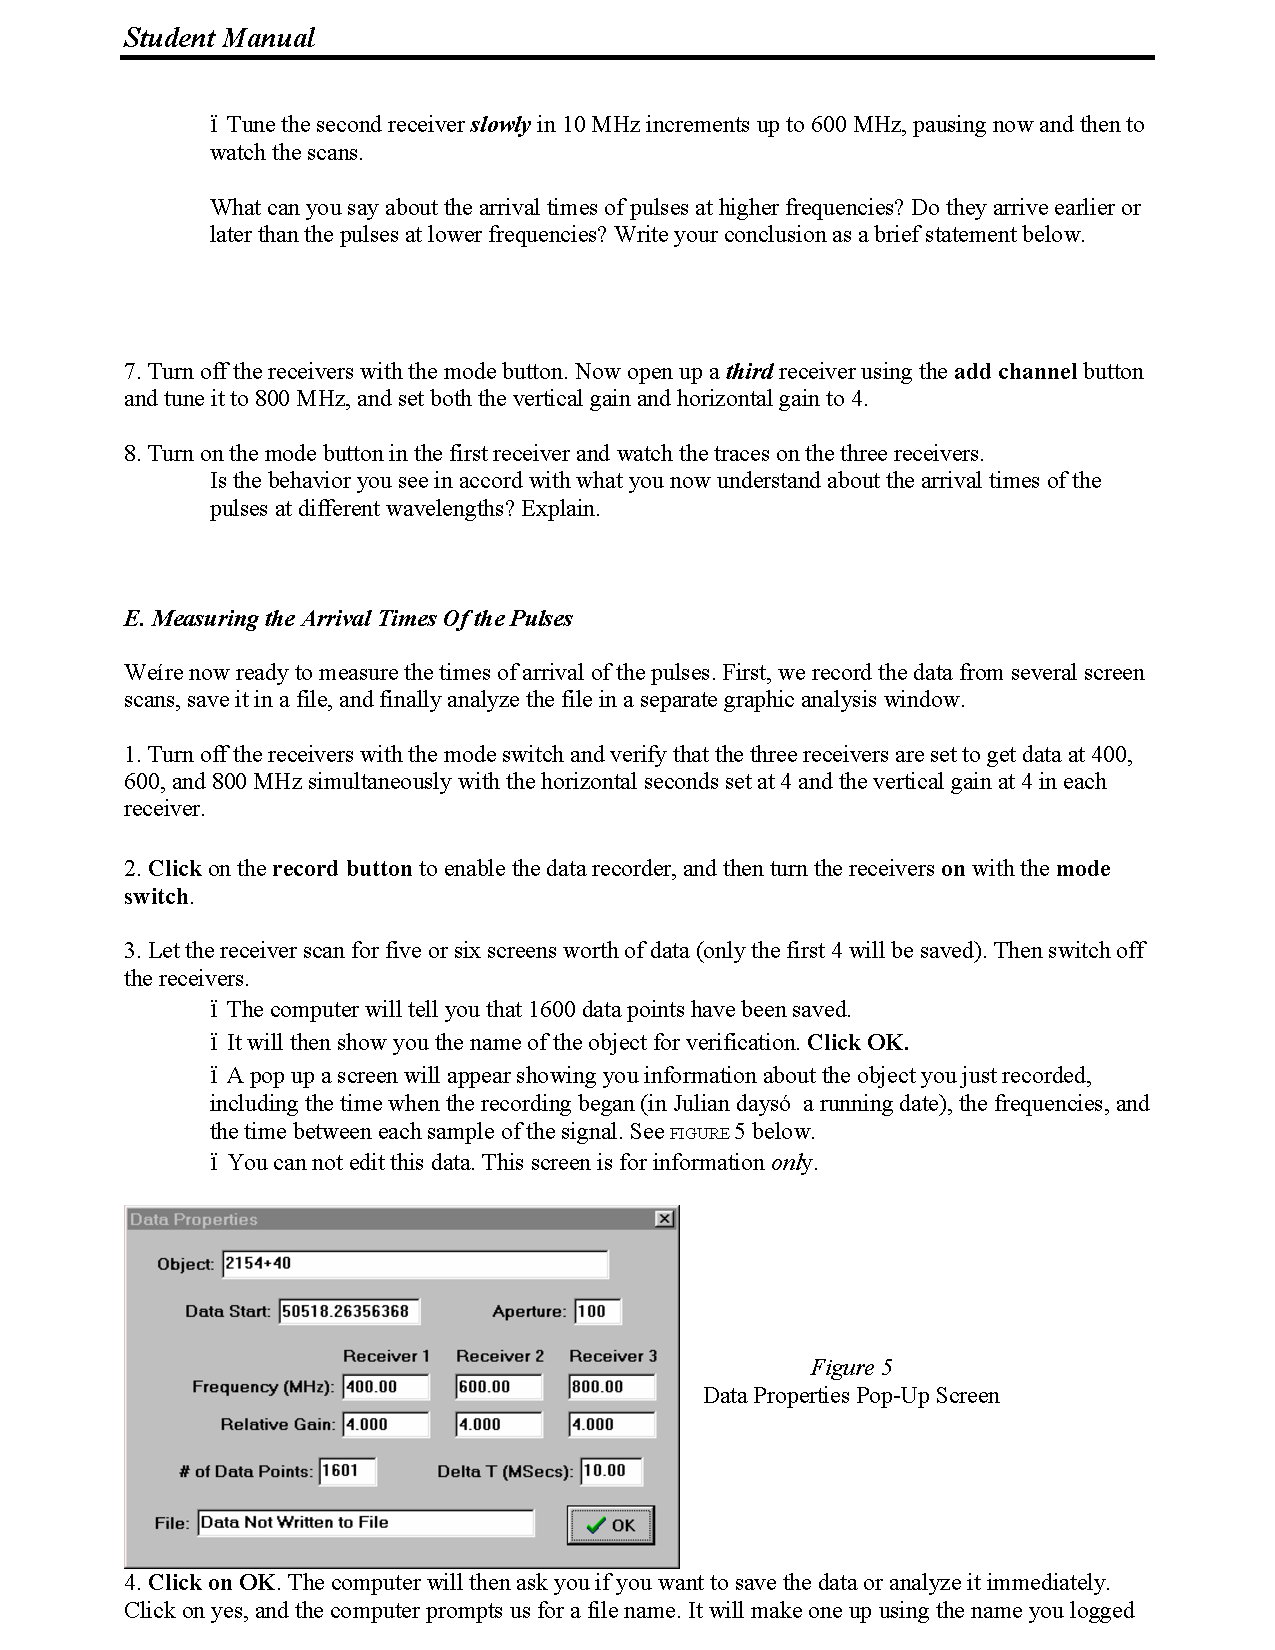
\includegraphics[width=\textwidth]{pulsars/pulsar10.pdf}
\vfil\eject

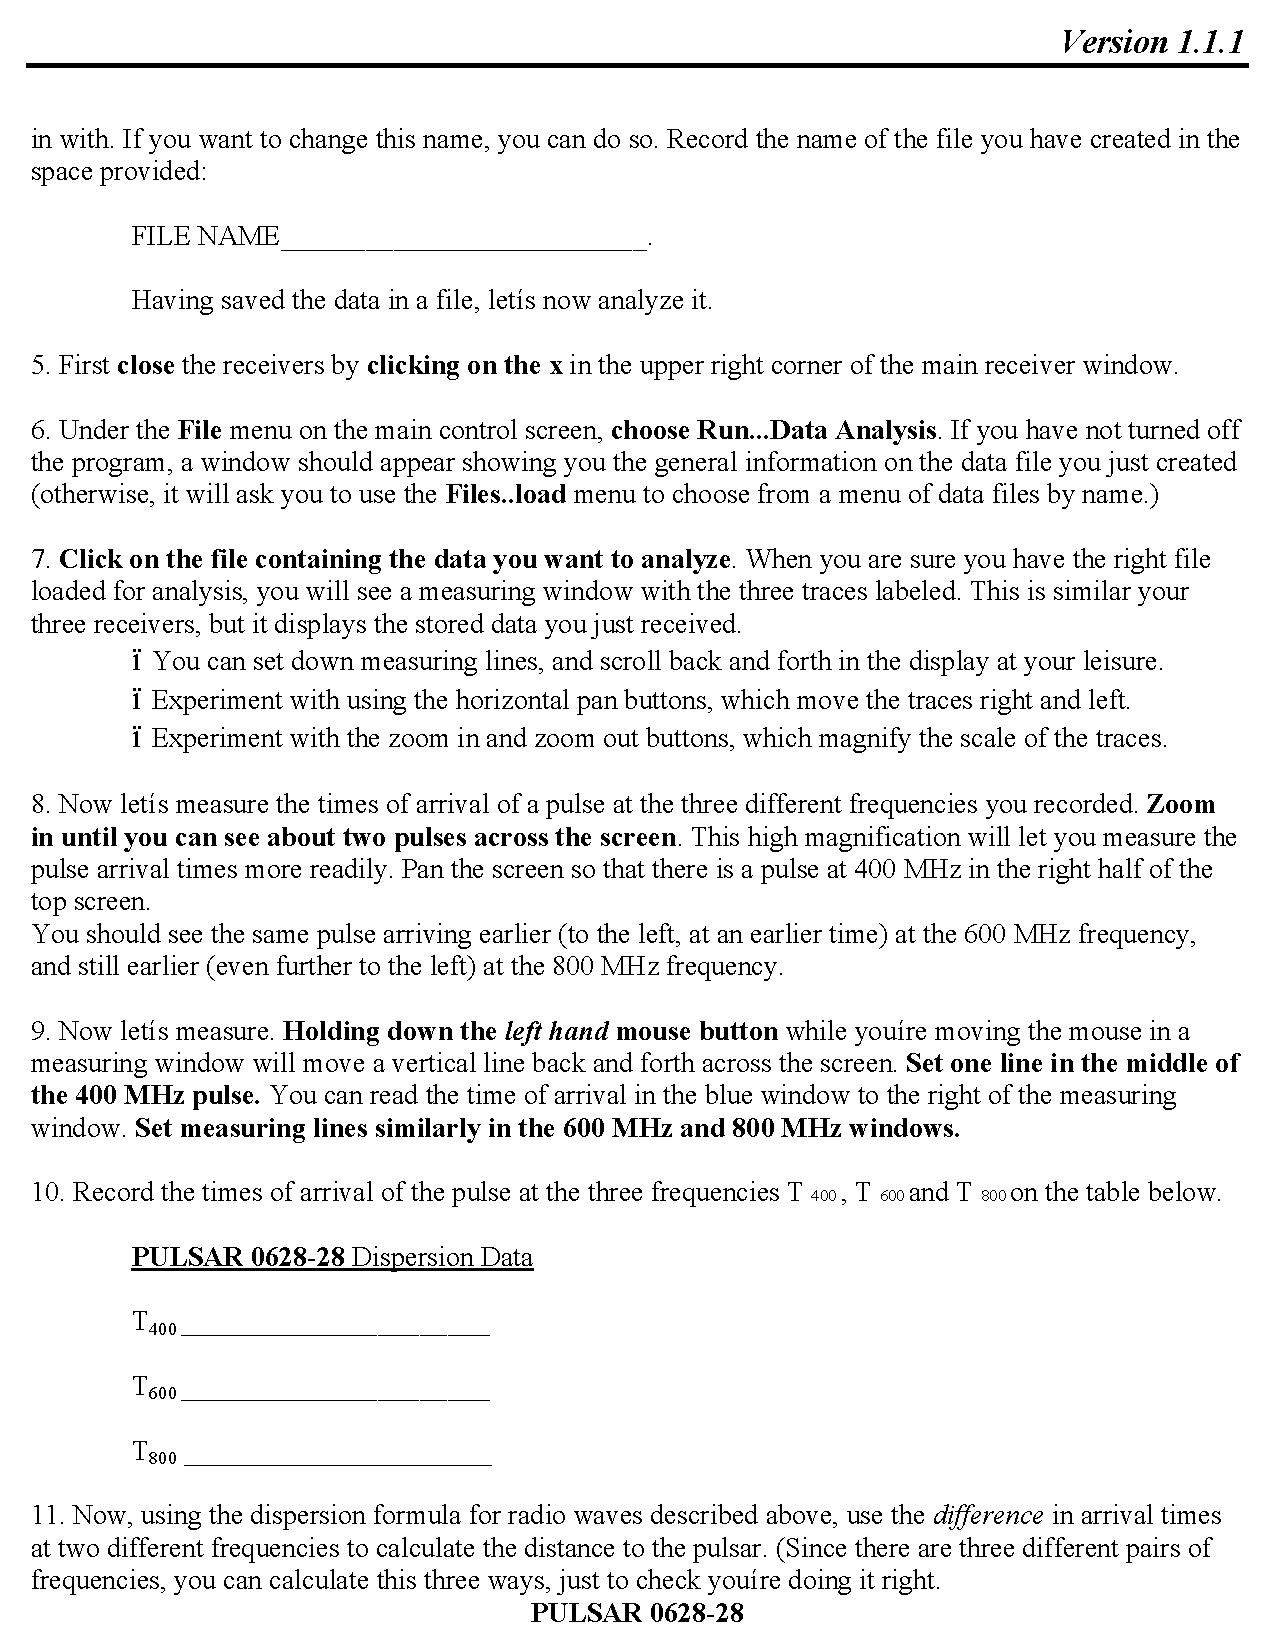
\includegraphics[width=\textwidth]{pulsars/pulsar11.pdf}
\vfil\eject

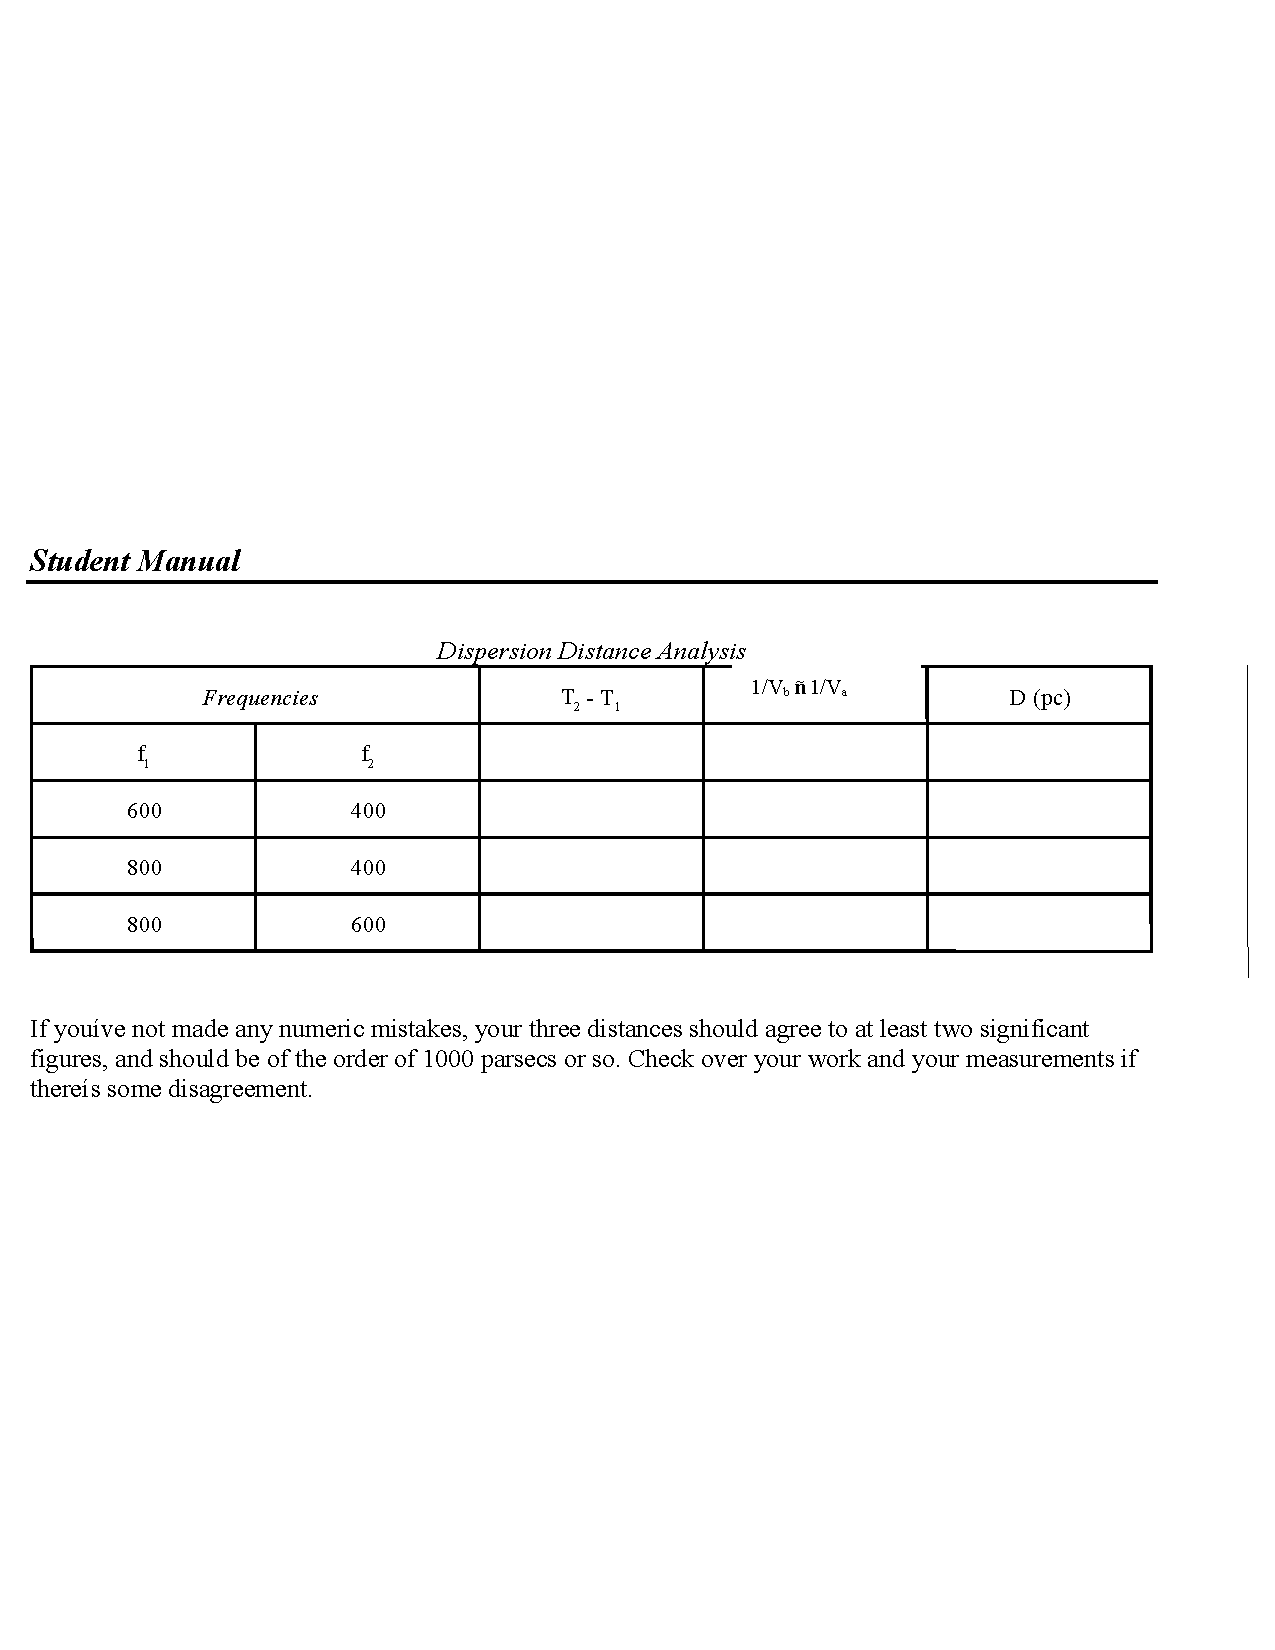
\includegraphics[width=\textwidth]{pulsars/pulsar12.pdf}
\vfil\eject

\chapter{The Crab Pulsar}


In this lab you'll use the same software as last time to examine the 
rotation period of the Crab pulsar.  In particular, you'll measure the
rate at which the pulsar is slowing down.
\bigskip\bigskip

{\bf Part 1: Period of the Crab Pulsar.}

Start up the radio telescope, turn on tracking, and use the Hot List to
point the telescope at the Crab pulsar (known to its friends as ``0531+21'').
Start up a receiver, and observe the pulses from this star.  Because this star
pulses very quickly, you'll need to set the {\bf Horz.\ Secs} level to 2.0.
Adjust the gain to some appropriate value.  Turn on the {\bf Record} button,
and start the receiver.  Let it run for at least four full traces across
the screen (8 seconds).  Once you have acquired your data, open it up
in the data analysis window.  You will use this data to determine the
period of the pulsar as accurately as possible.

First, zoom in as far as you can on the leftmost portion of the data.
Determine the time of the very first pulse (by dragging the vertical
cursor over the peak of the pulse).  The software is supposed to start
the clock right at the moment of the first pulse, so the time of this pulse
should be zero.  If this is not the case, talk to me.

Let's call that very first pulse ``pulse number zero.''  We'll
number all the pulses after it 1,2,3, etc.
Scroll forward to pulse number 20 and measure its time:

\medskip
$$
\mbox{Time of Pulse \# 20}=\hbox to 2in{}
$$
\medskip

Use this value to calculate the period of the pulsar:

\medskip
$$
\mbox{Period of Pulsar}=\hbox to 2in{}
$$
\medskip

Our goal today is to measure the {\it change} in the period
of the pulsar over time.  This change is very tiny, so we're going to
need to be highly accurate.  The number you just calculated for the period
isn't quite good enough.  

We could improve our measurement of the period if we count more pulses.
For instance, if you had measured the time of pulse \# 200 instead
of pulse \# 20, you'd get a better result.  It's tedious to count
200 pulses, though, so we'll use a shortcut.

Based on the value you found for the period, estimate the time at 
which pulse number 50 should occur.  (Don't count 50 pulses -- just
predict when it should occur.)

\medskip
$$
\mbox{Predicted time of Pulse \# 50}=\hbox to 2in{}
$$
\medskip

Now scroll ahead through your data to test this prediction.  Position
the cursor at the time you just calculated, and see if there's a pulse 
there.  You should find that there's a pulse at almost, but not exactly,
the time you predicted.  Measure the actual time of that pulse
as accurately as possible:

\medskip
$$
\mbox{Actual time of pulse \# 50}=\hbox to 2in{}
$$
\medskip

Note: you don't have to count the pulses to make sure this really is
\# 50.  Since you made a pretty accurate prediction of when \# 50
should occur, and you found a pulse at just about that time, you can
be confident you've got the right pulse even without counting.

Using the value you just measured the time of pulse \# 50, determine
the period of the pulsar.  This should be nearly the same as the
value you got before, but the new value is more accurate:

\medskip
$$
\mbox{Period of Pulsar (2nd estimate)}=\hbox to 2in{}
$$
\medskip

Record this value to at least four significant figures (for instance,
0.03283 seconds, although this isn't the right value).

We just ``leapfrogged'' from a 20-pulse estimate of the period to a 
50-pulse estimate.  Let's play that game one more time to get a 200-pulse
estimate.  That'll be accurate enough for our purposes.

Use your most recent estimate of the period of the pulsar to predict
when pulse \# 200 should occur:

\medskip
$$
\mbox{Predicted time of Pulse \# 200}=\hbox to 2in{}
$$
\medskip

Then go to that portion of your data, and find the pulse that's closest
to that time.  This is the

\medskip
$$
\mbox{Actual time of Pulse \# 200}=\hbox to 2in{}
$$
\medskip

From this value, determine yet another estimate of the

\medskip
$$
\mbox{Period of Pulsar (3rd estimate)}=\hbox to 2in{}
$$
\medskip

Record this value to at least five significant figures.

In principle, we could continue this ``leapfrog'' procedure, but
there's no need: this value is an accurate enough estimate.  There's
just one more bit of information we'll need: the uncertainty in this
measurement of the period (that is, an estimate of how far off
this number might be).  

One way to determine this is to measure the period several different times
and see how much it changes from measurement to measurement.  You
just determined the period by using the time of pulse \# 200.  
Determine it again using pulse \# 199 and pulse \# 201:

\medskip
\begin{eqnarray*}
\mbox{Time of Pulse \# 199}&=&\hbox to 2in{}\\
\mbox{Period determined from Pulse \# 199}&=&\hbox to 2in{}\\
\mbox{Time of Pulse \# 201}&=&\hbox to 2in{}\\
\mbox{Period determined from Pulse \# 201}&=&\hbox to 2in{}\\
\end{eqnarray*}
\medskip

Now that you have three different determinations of the period (from pulses
199,200,201), average them together to get your best estimate of the
true period.  Then figure out the uncertainty associated with this
value.  The uncertainty is how far off the worst of your three
measurements was from the mean.

Give your final answer here, in the form ``({\it Number}
 $\pm$ {\it Number}) seconds,''  with the two numbers being your
best estimate and its uncertainty.  Your best estimate should have five
significant figures.

\medskip
$$
\mbox{Final Value for Period (with uncertainty)}=\hbox to 2in{}
$$

\bigskip\bigskip

{\bf Part 2. The Period of the Pulsar in the Future.}

To see whether the Crab pulsar is slowing down, we need to wait
a while and measure the period again.  Since the slowdown is very
gradual, we need to wait a long time.  Five years works well.
Rather than actually waiting five years, which would be inconvenient,
we can tell the software to pretend that five years have gone by
and simulate data from a future date.

Close down the data analysis window and the receiver window.  Under
the {\bf File} menu, click on {\bf Date/Time}, and change the date to
five years from today.  After you've done that, you'll need to tell
the telescope to point toward the Crab pulsar again.

Now {\it repeat the entire procedure} to determine an accurate measurement
of the period of the pulsar, together with its uncertainty.

\newpage

\ \ \ 
\vfill

Based on the values you determined, {\it and their uncertainties},
can you conclude that the Crab
pulsar is slowing down?  (Is the difference between the two periods so great
that it lies outside the bounds of the measurement uncertainties?)

\vskip 1in

What is the rate at which the period is changing, in seconds per year?

\vskip 1in

The Crab pulsar was created in a supernova explosion in the year 1054.
Assuming that it has been slowing down at a steady rate ever since that
time, what was its period just after it was created?

\vskip 1in
\eject

\chapter{Black Holes}


\paragraph{Mass and radius.}
One of the key facts about black holes is the mathematical relationship
between the radius of the black hole and its mass:
$$
R_{\rm Sch}={2GM\over c^2}.
$$
The radius is called the ``Schwarzschild radius'' after Karl Scharzschild,
who first worked out the mathematics of black holes.  First, let's work out
Schwarzschild radii for some different sized black holes.  It's convenient
to group all of the constants together like this:
\begin{equation}
R_{\rm Sch}=\left(2G\over c^2\right)M.
\end{equation}
Remember that the gravitation constant is $G=6.67\times 10^{-11}\,{\rm
m^3/(kg\,s^2)}$ and the speed of light is $c=3.00\times 10^8$ m/s.
What is the numerical value of the combination $(2G/c^2)$, and what
are its units?  

(Remember how to determine the units: substitute the values of $G$
and $c$ into the expression $2G/c^2$, with their units, and then manipulate
the units algebraically just as if they were numbers or variables or anything
else -- for instance, cancel anything that appears in both numerator and
denominator of a fraction.)

\vskip 0.3in
$$
{2G\over c^2}=\qquad\qquad\qquad\qquad
$$
\vskip 0.3in

According to equation (1) above, you can convert any given mass into
the corresponding Schwarzschild radius by simply multiplying by this
value.  Are the units you found above consistent with this statement?
What units do you need to use for the mass?  What about for the radius?

\vskip 1in

What is the Schwarzschild radius for a black hole the mass of the Earth 
($5.98\times 10^{24}$ kg)?

\vskip 1in

A typical black hole that formed from a star has a mass of about 5 times
the mass of the Sun.  What is the Schwarzschild radius for such
a black hole?
(The Sun's mass is $1.99\times 10^{30}$ kg.)

\vskip 1in

The black hole at the center of our Galaxy may have a mass as high as 
$4\times 10^6$ solar masses.  What is its Schwarzschild radius?

\vskip 1in

Suppose we wanted to make a black hole whose radius was $10^{-10}$ meters
(about the size of an atom).  How much mass would we need?

\vskip 1in

\paragraph{Density.}
One way to get a feel for the extreme conditions required to form
a black hole is to consider the density of matter involved.
If we wanted to produce a black hole of a certain mass, we'd have
to compress all of that matter into a sphere whose radius was
equal to the Schwarzschild radius.  Remember that density is
mass divided by volume, and that the volume of a sphere is
$$
V={4\over 3}\pi R^3.
$$

Using this information, 
write down an expression giving the density required to form a black
hole in terms of the mass $M$.  Your expression should just have $M$
and constants such as $G$ and $c$ in it.  In
particular, it should not involve the radius $R$ --- 
if it does, use equation (1) to 
express the radius in terms of $M$.

\vskip 2in

Density = 

\vskip 0.5in

Note: It's not really correct to say that this is the {\it density
of the black hole} (although sometimes people do say this).  Rather,
it's the density of matter required to cause the black hole to form in
the first place.  After the black hole forms, all the mass gets concentrated
into a very small volume at the center, so the final central density after the
black hole has formed is much higher.

Does a very massive black hole require a larger or smaller density
than a not-so-massive black hole?

\vskip 1in

What is the density of matter required to form a 5-solar-mass black hole?
(Be sure to include units!)

\vskip 1in

What is the density of matter required to form a million-solar-mass
black hole?

\vskip 1in

What would the mass have to be if the required density is equal to the
density of water?  (Note: the density of water is 1 gram per cubic
centimeter, but grams per cubic centimeter are not the units you 
want to use in this expression!  If you're not sure how to express
the density in the correct units, ask me.)

\vskip 2in


You meet an alien from the Andromeda galaxy, who asks you the following
question: ``To make a black hole with a mass of 10 slurms, the required
density is 50 quatloos.  What density is required to make a black
hole with a mass of 40 slurms?''  You don't know how large a unit of 
mass a slurm is, nor do you know how large a unit of density a quatloo is.
Nonetheless, you can answer the alien's question.  What is the answer?

\vskip 2in



\paragraph{Orbital Periods.}
Black holes often have smaller objects orbiting around them.  When they do,
we can use the orbital periods to determine the black hole's mass
using Kepler's third law.  Remember Kepler's third law:
$$
P^2={4\pi^2a^3\over G(m_1+m_2)}
$$
For the next couple of calculations, it may help you to recall that
1 AU is $1.50\times 10^{11}$ meters and that 
1 year is $3.155\times 10^7$ seconds.

Suppose you observe a possible supermassive black hole at the center
of a galaxy.  A star is orbiting the center with an orbital radius of 1 AU
and is going at a speed of $6\times 10^7$ m/s.

What is the star's orbital period?

\vskip 2in

What is the mass of the black hole?

\vskip 2in

Express the radius of the star's orbit as a multiple of the 
black hole's Schwarzschild radius.  



\chapter{Galaxy Rotation Curves and Dark Matter}

\paragraph{Introduction.}

As you know by now, the way we (almost always) measure masses
in astrophysics is by measuring orbits and applying Kepler's Third
Law.  When we apply this technique to galaxies, we get a total
mass that is much larger than the mass of all of the visible
stuff we see.  This is the main way astrophysicists infer that
galaxies contain large amounts of unseen ``dark matter.''

In this lab, you will use observations of the spiral
galaxy NGC 3521 to figure out the mass distribution of the galaxy.
The data you will use was taken by Y. Sofue and collaborators
with a radio telescope in Japan.\footnote{In case you're
wondering, further information about the data is at
http://www.ioa.s.u-tokyo.ac.jp/$\sim$sofue/h-rot.htm,  but you don't
need to do anything with the information at that site.}
(This is real data, unlike
the various simulation labs we often do.)  

\paragraph{Useful facts for this lab.}

You'll need to use the small-angle formula,
$$
s={\alpha d\over 206,265}.
$$
You'll also need Kepler's Third Law,
$$
P^2={4\pi^2a^3\over G(m_1+m_2)}.
$$
Remember that in units of years, AU, and solar masses, the
constants $4\pi^2\over G$ come out equal to one and so can
be ignored.  Finally, some unit conversions:
$$
1\,{\rm pc}=206,265\,{\rm AU}.
$$
$$
1\,{\rm AU}=1.49\times 10^8\,{\rm km}.
$$


\paragraph{Procedure.}

\begin{enumerate}

\item Download and open the Excel file {\bf NGC 3521 rotation curve},
which is in the {\bf Downloads for labs} section of the Blackboard
site for this course.  This file contains measurements of the
radial velocity (the speed towards or away from us) of gas clouds
in this galaxy as a function of the clouds' distance from the center
of the galaxy.  The first column is the apparent location of the cloud
relative to the galaxy's center.  The fourth column is the speed
of that gas cloud towards or away from us.  (The speed is towards
us on one side of the galaxy and away on the other side.  Both
sides have been combined in this data set.)

\item How do you think that the speed information was obtained?

\vskip 1in

\item You'll need to know the actual distances of the various gas clouds
from the center of the galaxy.  Use the small-angle formula to figure
those out in both kiloparsecs and AU, entering the results in the
second and third columns of the spreadsheet.  The distance to the
galaxy NGC 3521 is 8900 kpc.  Since there are many rows of data, you'd
be very unwise to do this step one row at a time; use an Excel formula
to do them all at once.  See Appendix C for reminders about how to do this sort
of thing.

\item Plot a graph showing the distance from the center in kpc on the
$x$ axis and the rotation speed on the $y$ axis.  Be sure that
the axes of your graph are clearly labeled including both the
name of the quantity being plotted and its units.  This graph
is called the ``rotation curve'' of the galaxy.

\item Using another Excel formula, 
create a new column in the spreadsheet giving the period
of the orbit of each gas cloud in years.  (The orbits can
all be assumed to be circles.)  As usual, be sure the column
is labeled with both a name and units.

Your formula will probably give an error in the very first line,
because the radius and speed are both zero there.  That's OK,
as long as it gives correct results for the other lines.  The
same thing is true for the next step.

\item Next you will use Kepler's Third Law to determine the mass contained
within each gas cloud's orbit.  Create a new column to contain
this information, and use an appropriate Excel formula.

\item Plot a graph showing the distance from the galaxy's center
in kiloparsecs on the $x$ axis and the mass on the $y$ axis.

\item From your graph, it should be clear that something has gone 
wrong at large distances.  Explain how you know.  (What does the graph
do at large distances?  Why is this impossible?)

\vskip 1.5in

As it turns out, the data are reliable out to about 17 kpc.

\item Other measurements have been made to determine the 
distribution of light coming from this galaxy.  They have determined
that 90\% of the total light from the galaxy comes from the
innermost 9 kpc of the data.  Assuming that the maximum value
of mass you found is the total mass of the galaxy, what percentage of the
total mass of the galaxy lies within 9 kpc of the center? 
Based on this information, would you conclude that the total mass
in the galaxy is more spread out than the stars, or less spread out?

\newpage
%\line{\ }

\vskip 1.5in

\item In answering the previous question, you assumed that the
largest mass value you found was equal to the total mass of the galaxy.
That might be wrong: the graph of mass might continue to go up if
we had reliable data at greater distances.  If you did discover
that the total mass of the galaxy continued to go up as you observed
out to greater distances, would it strengthen or weaken
the conclusion you drew in the previous question?

\vskip 1in

\item The luminosity of this galaxy is about $1.5\times 10^{10}$
times the luminosity of the Sun.  Calculate the ``mass-to-light
ratio'' of this galaxy by dividing the total mass (in solar masses)
by the total luminosity (in solar luminosities).  

\vskip 0.5in

\item If the galaxy were made
up of nothing but stars just like the Sun (with no gas, dust,
or dark matter), what would the mass-to-light ratio be?

\vskip 0.5in

\item Astrophysicists think that a typical collection of gas,
dust, and stars in a galaxy (with no dark matter) 
should have a mass-to-light ratio of about 2.  Assuming that
that's correct, use the luminosity to 
determine the mass of all of the gas, dust, and
stars in this galaxy.  How many times greater is the total mass
of the galaxy than the mass of all the visible stuff?

\end{enumerate}



\chapter{Hubble's Law}

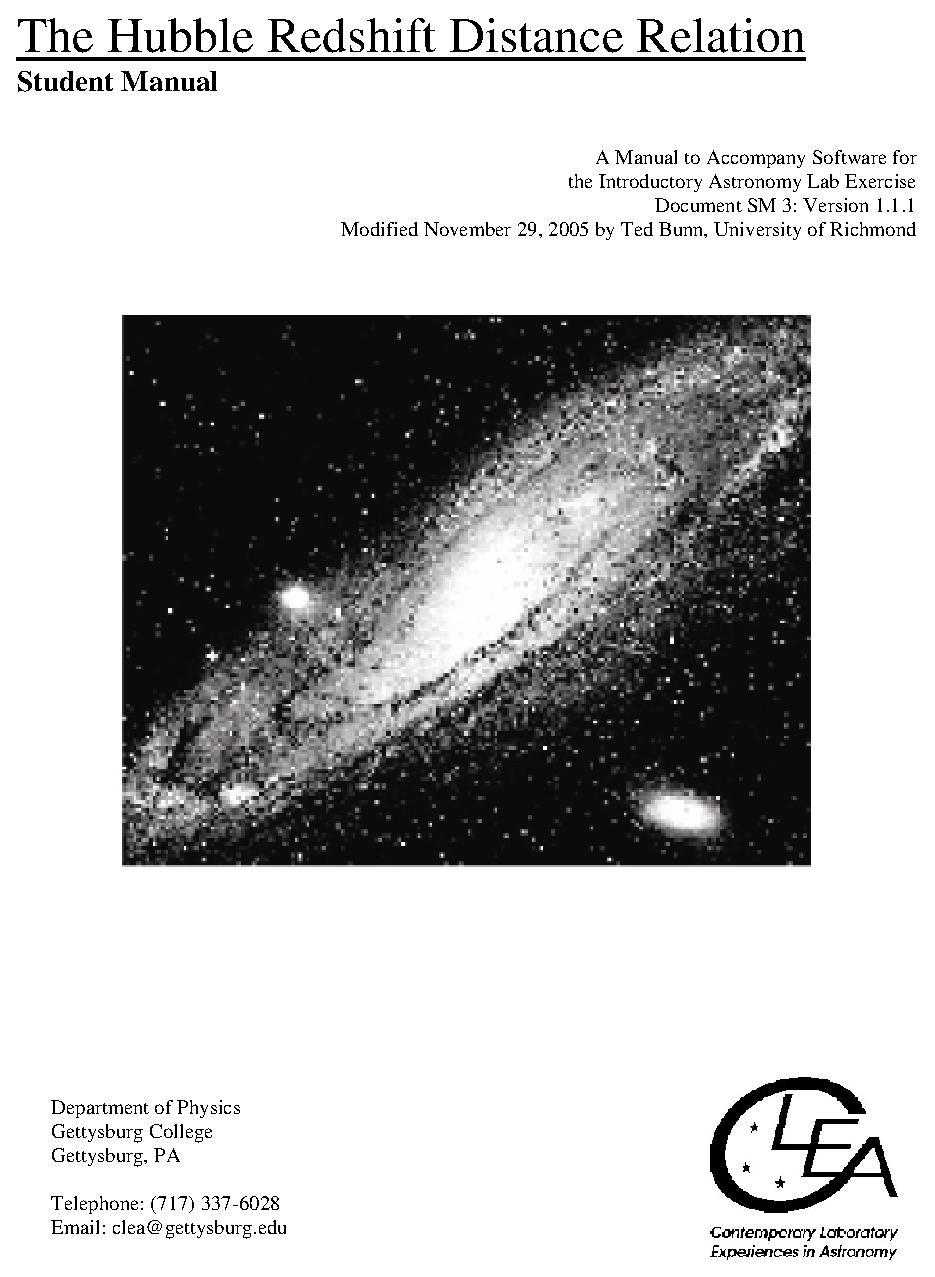
\includegraphics[height=6.3in]{wordtops/hubble1.eps}

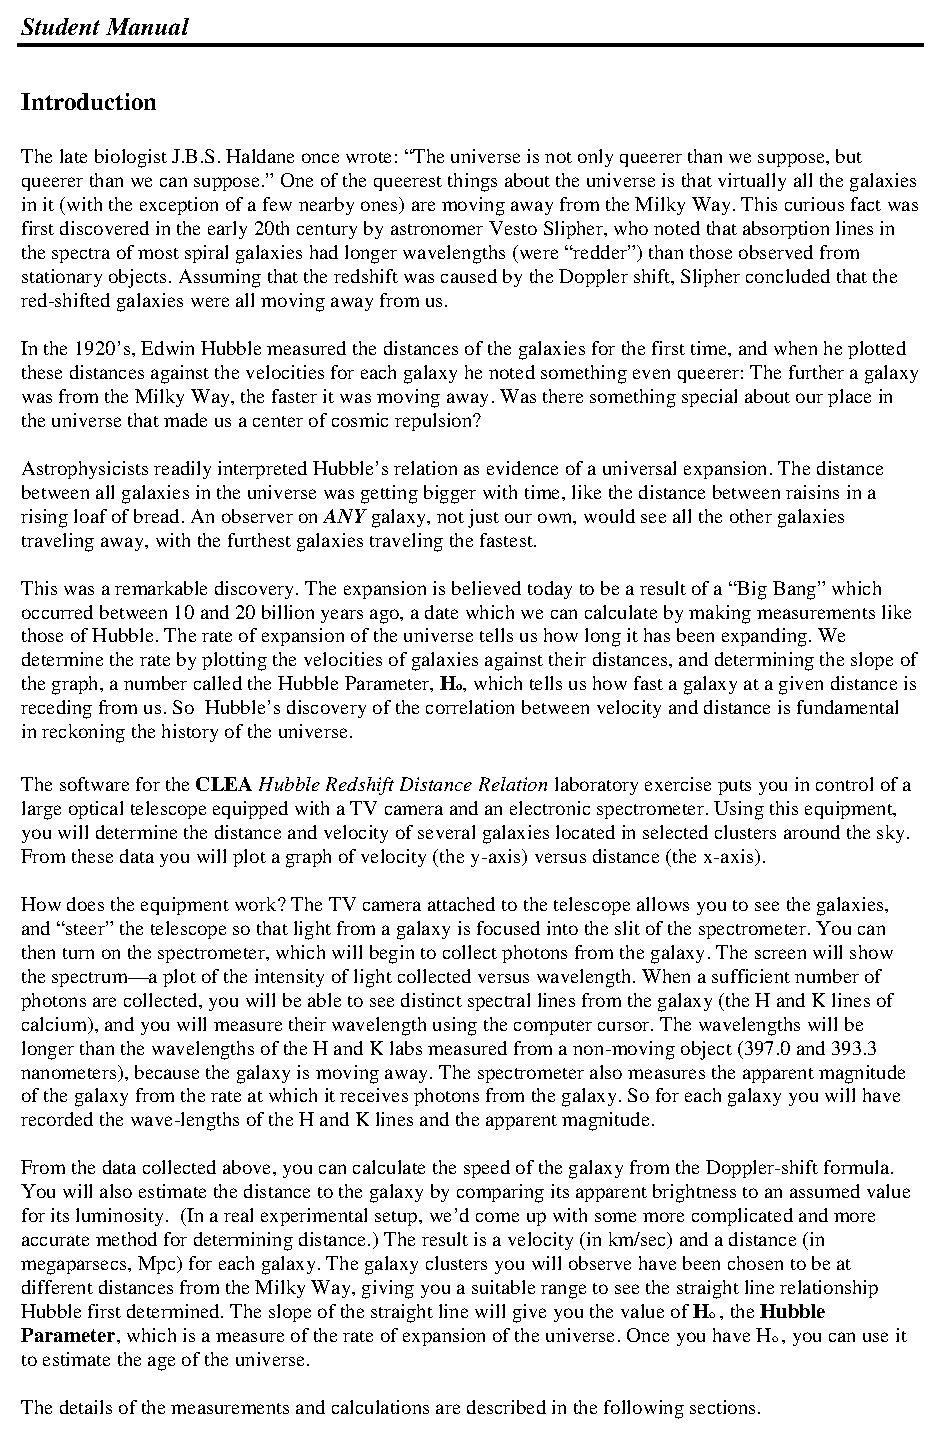
\includegraphics[height=9in]{wordtops/hubble2.eps}

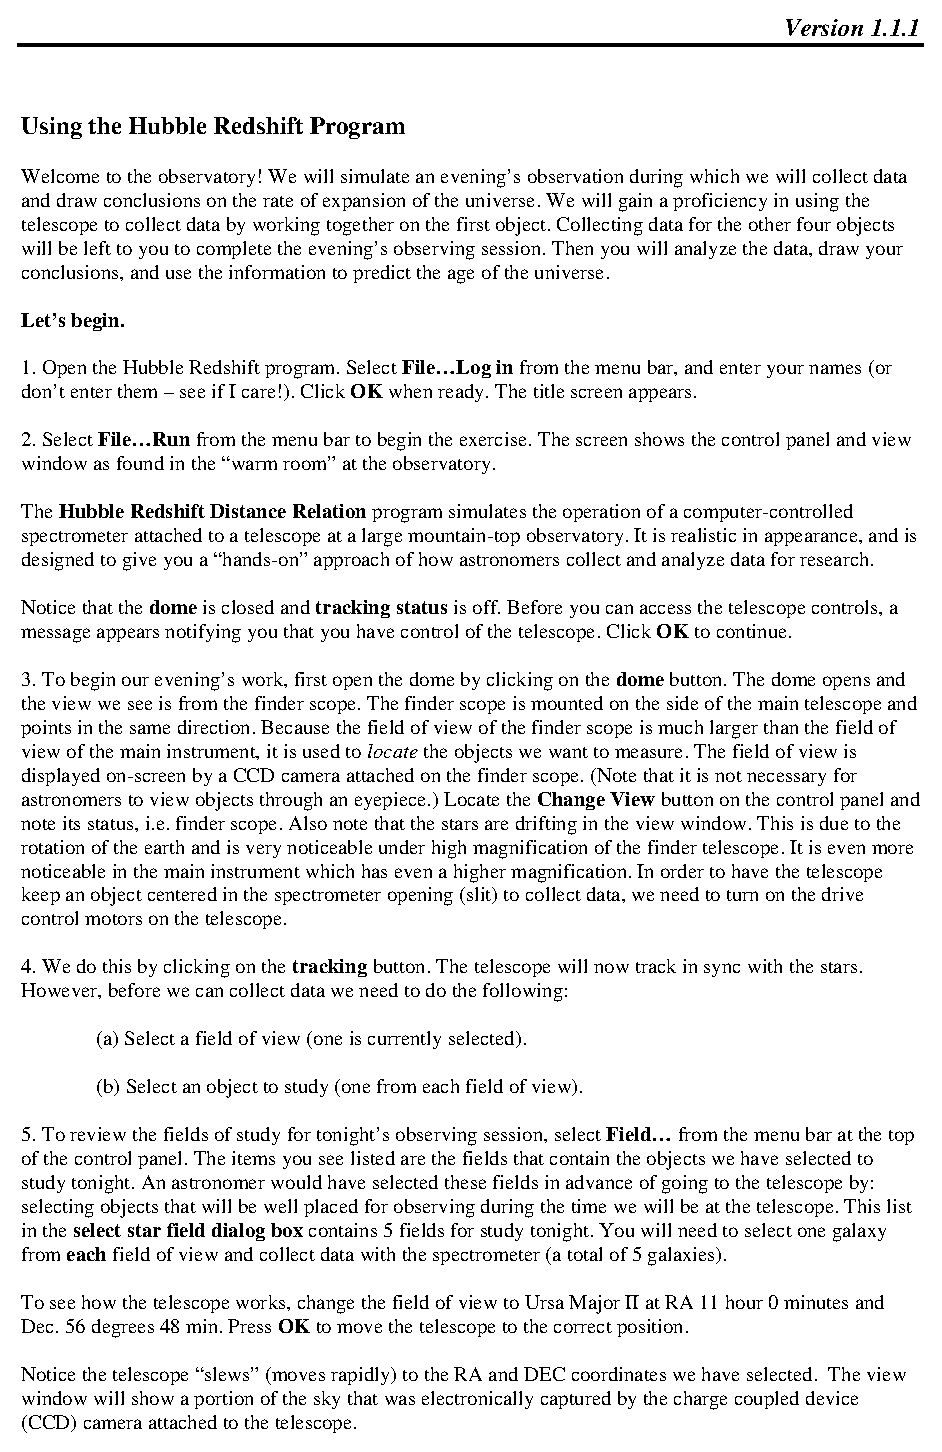
\includegraphics[height=9in]{wordtops/hubble3.eps}

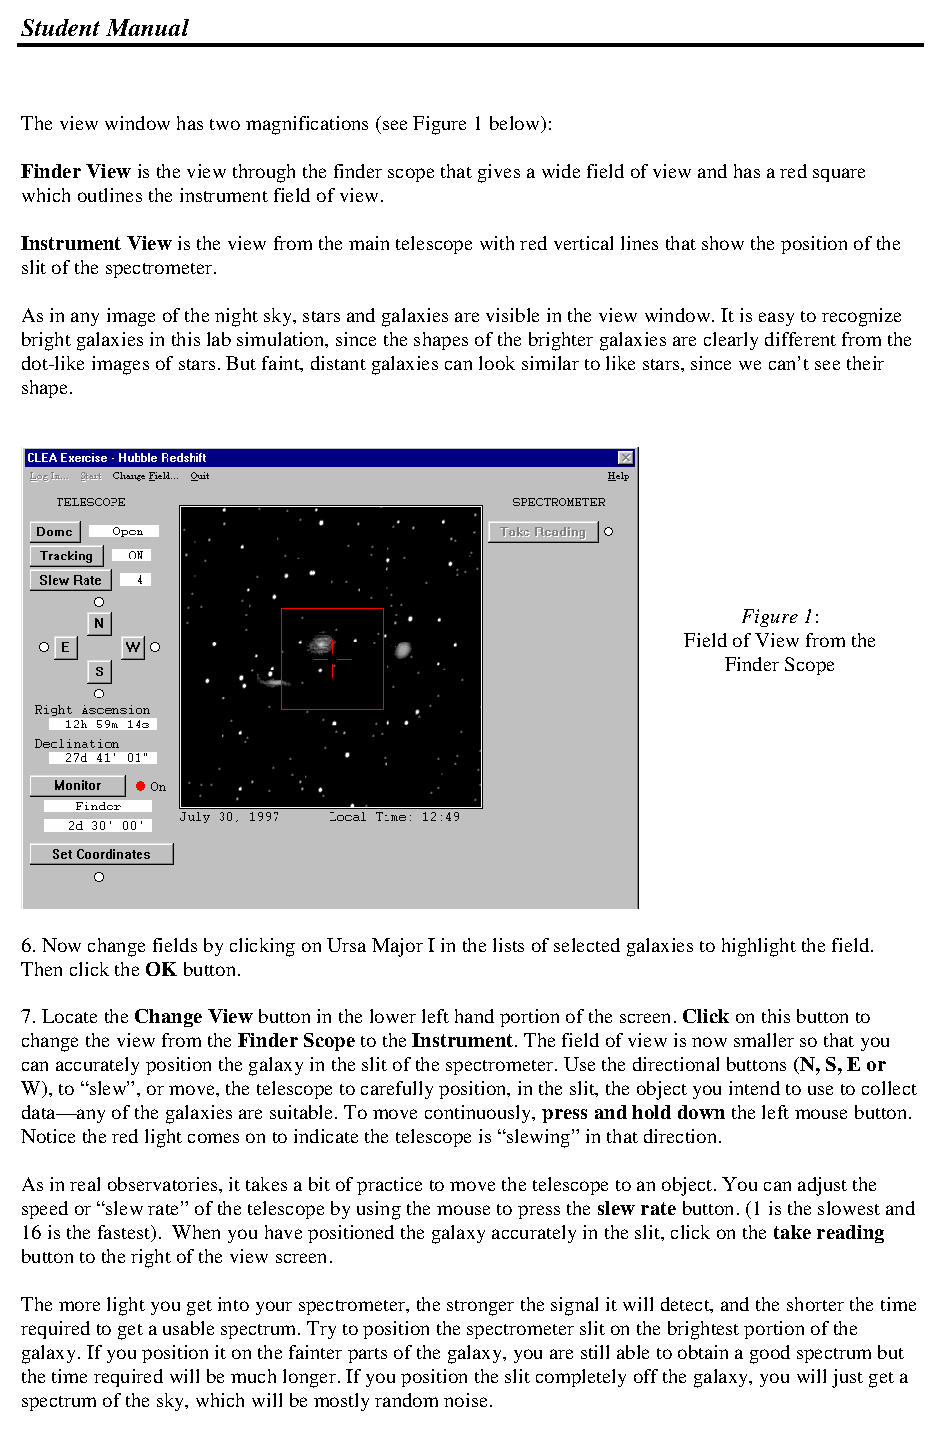
\includegraphics[height=9in]{wordtops/hubble4.eps}

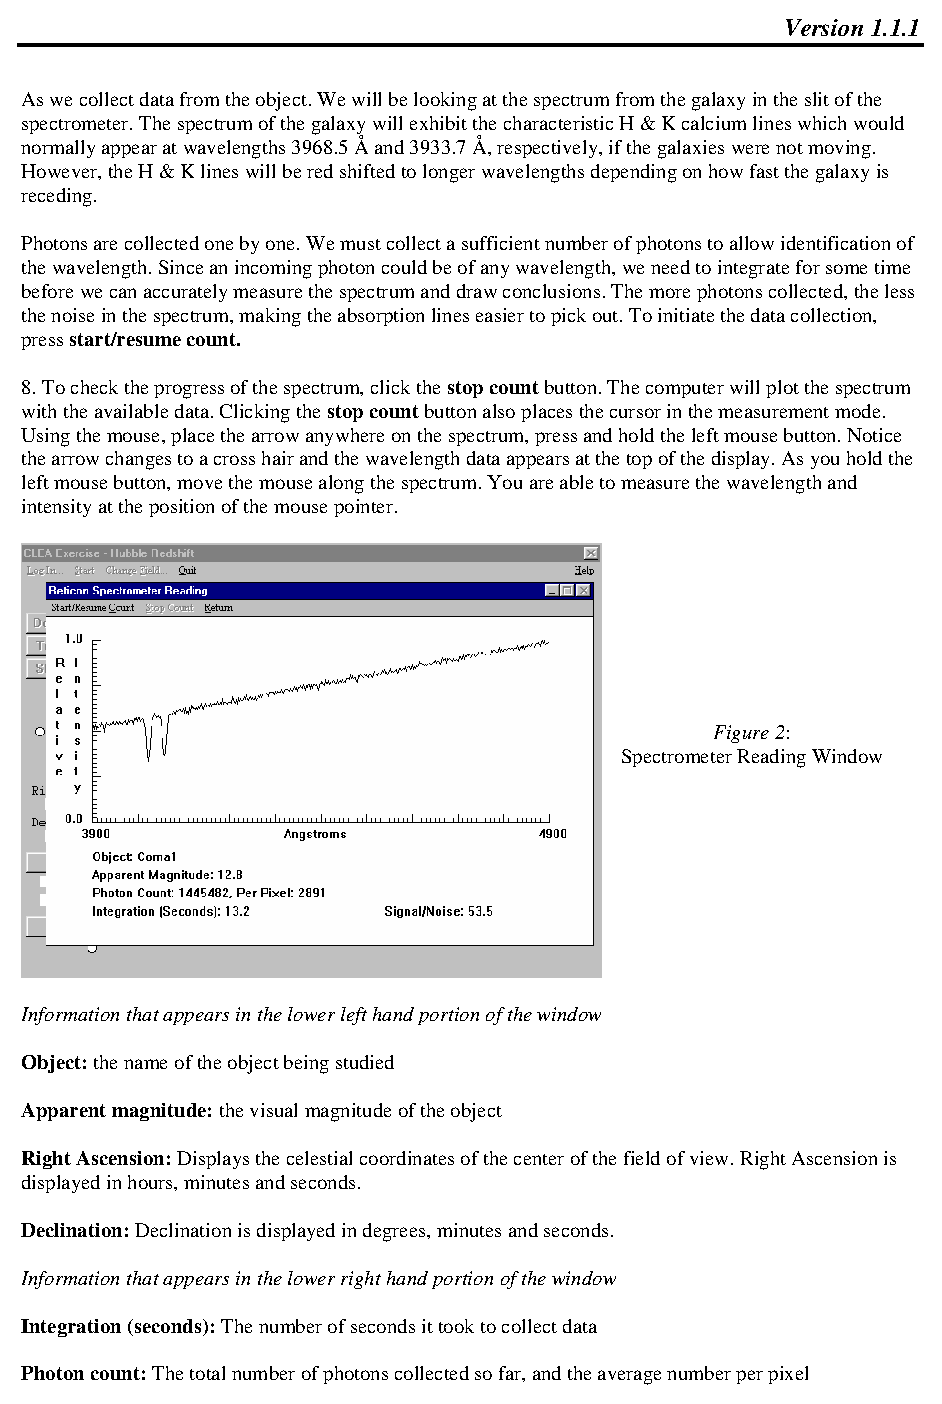
\includegraphics[height=9in]{wordtops/hubble5.eps}

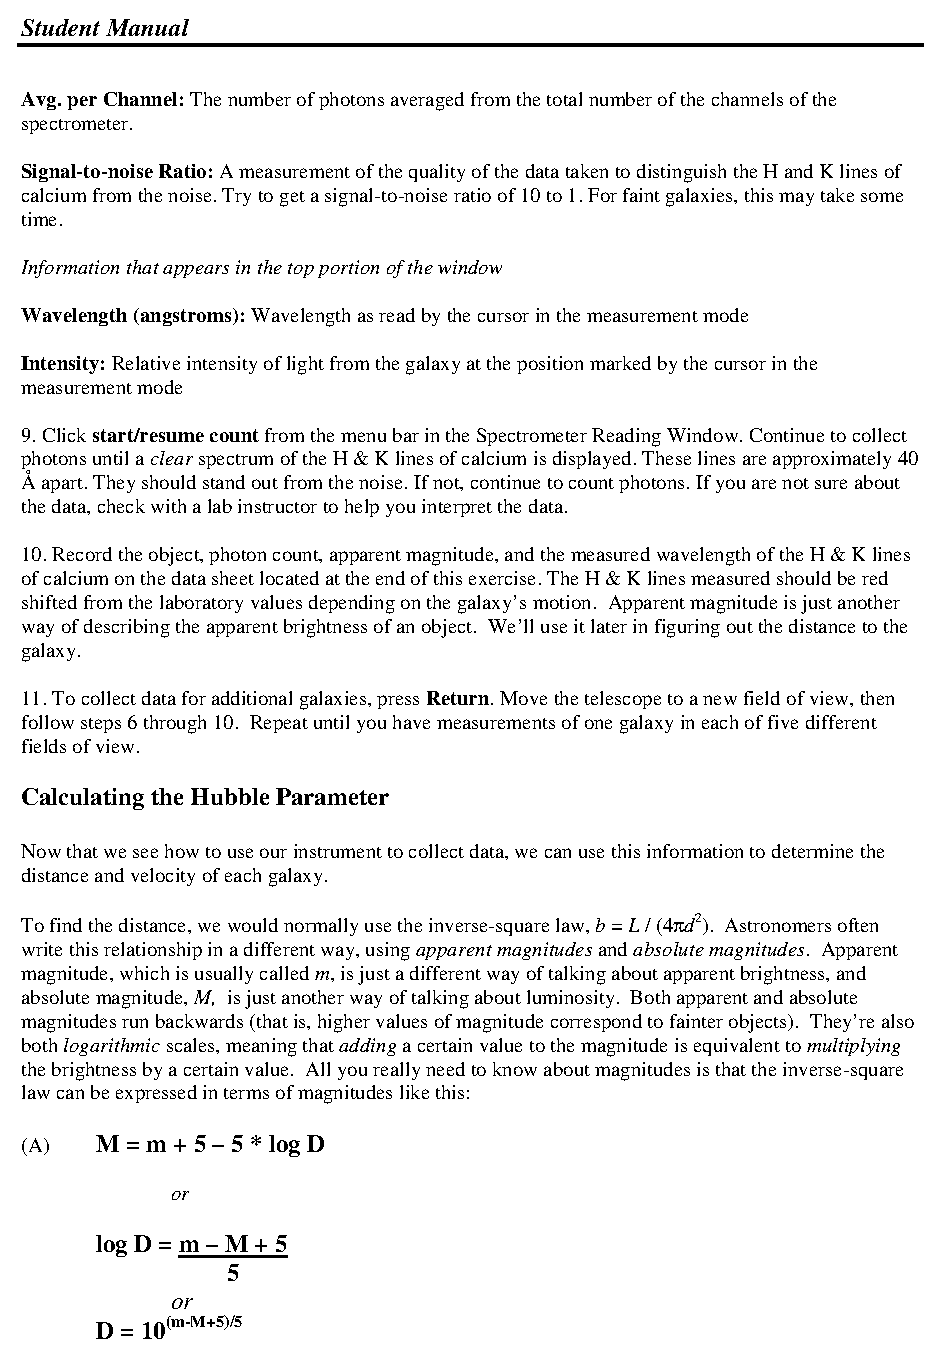
\includegraphics[height=9in]{wordtops/hubble6.eps}

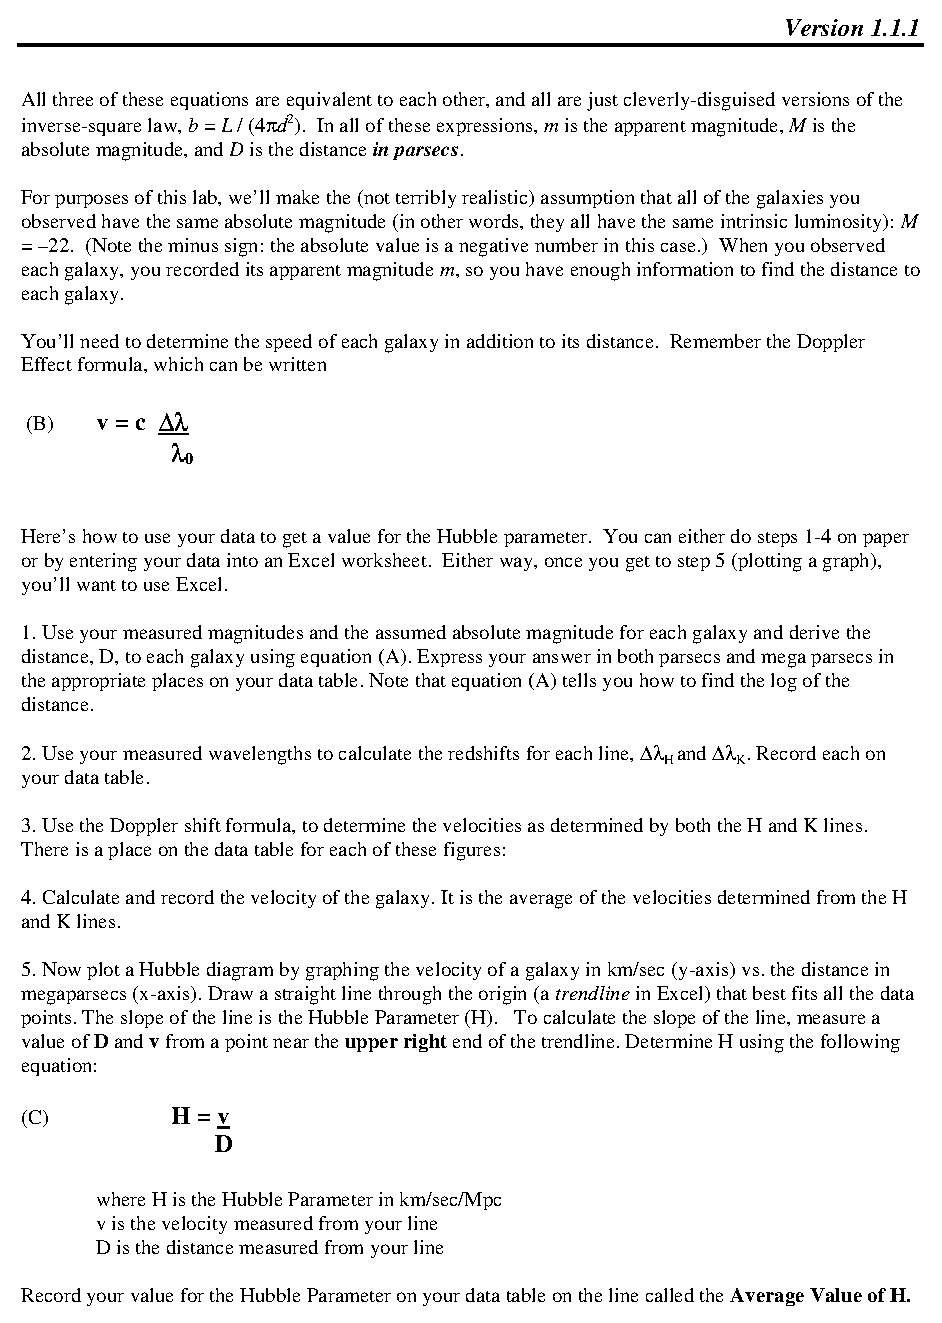
\includegraphics[height=9in]{wordtops/hubble7.eps}

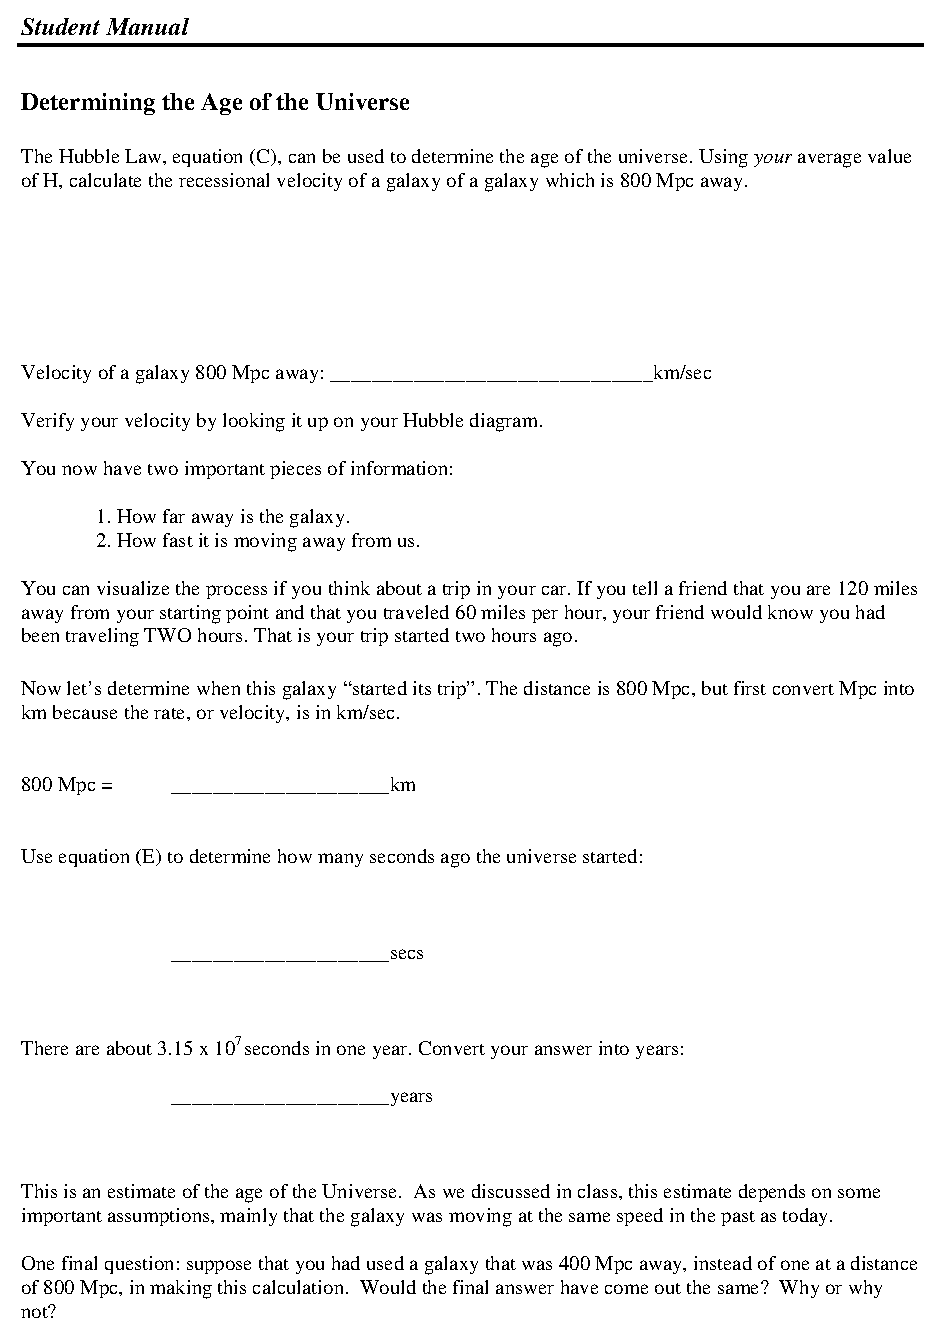
\includegraphics[height=9in]{wordtops/hubble8.eps}

\includegraphics{wordtops/hubble9.eps}

\section{Are We Alone?}

\makelabheader

\bigskip

As far as we can tell, our Sun is a fairly typical star in a fairly
typical galaxy.  The Universe contains a huge number of stars very much
like our own.  Do any of them have life?  Nobody knows, but that doesn't
stop us from trying to find out!

First, let's get a feel for the number of stars in the Universe.
Here are some useful numbers to get us started:

\begin{itemize}
\item There are about 300 billion stars in our own Milky Way Galaxy.
\item The observable Universe is a sphere with a radius of about
5000 megaparsecs.
\item There's about one large galaxy like our own for every 100 cubic
megaparsecs (Mpc$^3$) of volume.
\end{itemize}

About how many large galaxies are there in the observable Universe?

\answerspace{1.5in}

Assuming all of those large galaxies have about the same number
of stars as our own Galaxy, about how many stars are there in the
observable Universe?

\answerspace{1in}

Suppose that a star has a one-in-a-million chance of having
a planet that develops life.
How many stars in our Galaxy have life?

%\vskip 1in
%\newpage

Continuing to suppose that a star has a one-in-a-million chance
of developing life, how many stars in the observable Universe have life?

\answerspace{1in}

Now suppose that life is less likely: say that only one in a trillion
($10^{12}$) stars develops life.  How many stars in the observable Universe
have life?

\answerspace{1in}

Of course, the problem is that we have no idea what the probability
of life developing around any given star is.  It could be
one in a million, one in a trillion, or something much larger or much smaller!

Suppose that there are planets out there with life on them.  How could we
detect them?  If we were really lucky, maybe the creatures on them
would have developed a technological society similar to ours.  
In that case, they might actually send out radio broadcasts
into the Galaxy, to see if anyone's out there.  Even if they
didn't do that, 
they might use radio waves to communicate with each other (just 
as we do).  In that case, we
might be able to detect their broadcast signals.  (Just as an alien
civilization 20 light-years away might just now be receiving our radio
and television broadcasts from 20 years ago.  I wonder if they like
``Seinfeld.'')

Back in 1961, the astronomer Frank Drake wrote down an equation that
can be used to estimate the number of alien civilizations that we might
hope to detect in this manner.  Here's one way of writing the {\it
Drake Equation}:
$$
N_c=N_*f_pn_ef_lf_if_cf_L.
$$
Here's what this means.

The quantity $N_c$ is the number of civilizations in our Galaxy
from which we might possibly be able to detect signals.  That's what
we want to find.  The things on the right are
\begin{itemize}
\item $N_*$ is the number of stars in our Galaxy.
\item $f_p$ is the fraction of all of those stars that have planets.
\item $n_e$ is the average number of planets around each such star
that can sustain life.  (One way people often interpret this term
is that it's the number of planets with liquid water.  It's much
easier for the complex chemical reactions that cause life to occur
if there's liquid water around.)
\item $f_l$ is the fraction of all of such planets on which life actually
evolves.
\item $f_i$ is the fraction of all such life-containing planets on which
{\it intelligent} life arises.
\item $f_c$ is the fraction of all such intelligent-life-containing
planets where the inhabitants are communicating with us.  (This could mean
either the fraction that are deliberately beaming signals out into space
to let us know they're there, or the fraction that are using 
broadcast signals to communicate with each other.)
\item $f_L$ is the fraction of the Galaxy's life during which
the civilization is communicating.  The life of the Galaxy so far is
about 10 billion years, so this last term is the lifetime of the
technologcal civilization divided by 10 billion years.
\end{itemize}

Although this equation looks complicated and 
has a lot of terms in it, I hope it makes sense where all the terms come from.
Most of the terms (all the ones called $f$) are fractions that could
be anywhere from 0 to 1.

The problem is that we have very little idea what a lot of the numbers
on the right side of this equation should be!  

For instance, maybe
life evolves pretty much every time it possibly can, so that every
planet that can possibly sustain life does in fact evolve life.
If that's true, then $f_l$ would be about equal to 1 (that is, 100\%).  
On the other hand,
maybe it takes an incredible stroke of luck for the molecules on a planet
to organize themselves in such a way that life gets started.  If that's
true, then $f_l$ would be an extremely small number.

Similarly, it might be the case that intelligent life is very rare
-- maybe there are lots of planets oozing with bacteria but very few
with big-brained creatures like us.  In that case, $f_i$ would be small.
Or maybe once life gets started it's inevitable that it grows in complexity
until something intelligent arises.  In that case, $f_i$ would be nearly equal
to 1.

\pagebreak[2]

Using Google (or some other search engine), dig around the web for a while
to come up with a range of plausible estimates for these numbers.\footnote{Just
in case there's any doubt, let me mention that ``dig around the web''
is not generally considered to be part of a good scientific methodology.
In this case, though, we just don't know what the right answers are,
and I just want to get an idea of a plausible range of answers.}
  (``Drake
equation'' is a good search term.  Be warned: there are slightly
different ways of writing the equation, with different choices
of symbols for the various quantities.)  Feel free to use your own
judgment along with anything you find on the web.
Let's assume
that the number of stars in our Galaxy is known to be 300 billion:
$$
N_*=3\times 10^{11}.
$$
For each of the other numbers, list two values: a ``pessimistic'' estimate
and an ``optimistic'' one.  There's not one right answer for these,
of course!

\begin{itemize}
\item $f_p=$
\item $n_e=$
\item $f_l=$
\item $f_i=$
\item $f_c=$ 
\item $f_L=$ 
\end{itemize}

Using all of your low numbers, estimate the number $N_c$ of communicating
civilizations.  Then use all of your high numbers to estimate the number.
Give a range of plausible values for $N_c$:

\answerspace{1in}

There is an ongoing project called the Search for Extraterrestrial
Intelligence (SETI) looking for radio signals from intelligent beings
on other planets.  Based on your estimates, do you think SETI is likely
to succeed?  


\appendix
\renewcommand{\chaptername}{Appendix}
%\chapter{Introduction to Sky Safari}
\newcommand{\skysaf}{\textit{Sky Safari$+$}}
\newcommand{\icon}[1]{\includegraphics[height=0.2in]{figs/stell-#1.eps}}

\bigskip\bigskip

\skysaf\ is an iPad / Android app that simulates the appearance
of astronomical objects in the sky. The user can adjust lots of
features of the view, including the observer's location,
the time, etc. We'll make heavy use of it as we try to understand
how objects appear to move in the night sky.

Although it's certainly not required, 
I encourage you to download it onto any suitable device
you own. \skysaf\ is not free, but it doesn't cost much.
There is a free version
of \textit{Sky Safari} that does many but not all of the things we'll want.

In this Appendix, I'll list some of the features of the program that will
be most useful to us. The best way to learn about these features is not
just to read about them here, though. Spend some time playing around, to learn
what you can do.


\paragraph{Moving around the sky.} 
This all works in the way that you're surely used to.
Drag across the screen to change what area you're looking at,
and zoom in and out using the usual two-fingered pinching motion.

Note that the ``Field of View'' (FOV) is indicated
at the upper right (something like $99.3^\circ\times 76.1^\circ$, for
instance). The FOV is the size (in degrees) of the
patch of sky that's visible on the screen at that moment.

\paragraph{Selecting and centering on an object.}
You can select a star or planet (or other celestial object)
by tapping it.
If you hit the ``Info'' button at the bottom,
you'll get a bunch of information about the object
(more than you wanted to know).
If you hit the
``Center'' button, the object will be moved
to the center of the screen. Once an object has been centered, it will
stay centered until you choose a new object or drag to view
a different part of the sky.

\paragraph{Changing the observer's location.} Hit
``Settings'' and then select ``Location'' to 
choose where the observer is located. You can either enter latitude
and longitude or choose a city from a list. 

\paragraph{Changing time.} Hit the ``Time''
button to bring up a set of options for adjusting the time.
The ``Now'' button, unsurprisingly, will return the time to the present.
The button to the right of ``Now'' will advance the time forward
by one step. The buttons in the next row let you choose the step size to be a year, month, day,
hour, minute, or second. The button to the left of ``Now'' steps
backwards.
The triangular buttons on the left and right make time advance 
steadily, with a speed that depends on the step size you've chosen.
In case it's not clear what this means, select ``Hour'' and then
hit the triangular button. Then select ``Minute'' or ``Day'' and
see what happens.

The date and time are indicated in the upper right.

\paragraph{Finding a specific object.} Hit the search button
and enter the name of the object you're looking for.

\paragraph{Miscellaneous display options.} 

You can find all of these under the ``Settings'' menu.

The ``Horizon \& Sky'' tab under ``Display Options'' lets you customize
how the Earth's surface is displayed. If you turn off the ``Show 
Horizon \& Sky'' option, then you'll get to see how things would
look if the Earth were invisible. That is, you'll get to see even
the stars that lie below the Earth's surface. 
You can also turn on and off the effects of daylight. With daylight turned
off, you can see the stars as they would appear during the day.
Of course, these are things we can't do in real life
(no matter how much astronomers wish we could), but they're
useful tools for helping to build intution about how
objects move in the sky.

By default, the program is set up to show you the horizon as a 
(somewhat) realistic landscape. Sometimes it's nicer to see what
things would look like if we were surrounded by a completely flat horizon
(no hills, trees, etc.). To do this select the option to show
the horizon as an ``opaque area.''

The ``Constellations'' tab under ``Display Options'' lets you
change how constellations are indicated.
In particular, you can turn on or off the display of names
of constellations (``Show constellations''). You can also have
the program display lines connecting the stars in a constellation or even
indications of the mythical figures that the constellations represent.
Personally, I don't think the last one is very helpful, but
some people like it.

Astronomers label points in the sky with two kinds of coordinates, 
which \skysaf\ calls ``horizon coordinates'' and ``equatorial coordinates.''
In other sources, you'll often see ``horizon coordinates'' called
``azimuthal coordinates.''
We'll talk about these in detail in class,
but for the moment here are the basics.
Both of these are like latitude and longitude on Earth. The
difference is that the equatorial grid is ``attached'' to the sky, so
that each star's coordinates stay the same as time passes.
The
horizon (or azimuthal)
grid, on the other hand, is attached to the Earth. 
The ``Grid and Reference'' tab under ``Display Options''
lets you turn on and off a grid showing either one of these coordinates.


\paragraph{Measuring angles.}
Often, we want to know the \textit{angular separation} between two
objects in the sky. Angular separation is the angle between a line from your eye
to one object and a line from your eye to the other object; it's a measure
of how far apart the objects appear to be. To determine
angular separation, select the the first object, then
select the second, and then hit the ``info'' button. Near
the bottom of the information screen, you'll find the angular separation.

For instance, to find the angular separation between Jupiter and Saturn,
you'd tap Jupiter, then Saturn, then ``info.'' Then you'd
look for the line that says
``Angular separtion from Jupiter.'' (It'd say ``from Jupiter''
because it's currently displaying information \textit{about}
Saturn. In general, you want the line that refers to 
angular separation from the first object you tapped.)

\paragraph{Stationary-Earth and stationary-sky points of view.}
As we'll see in detail, objects in the night sky appear to rotate
approximately once per day about a point in the sky called the ``north
celestial pole.'' This apparent motion is due to the 
Earth's rotation on its axis: the stars are really (more or less)
sitting still. 
Often, it's useful to examine what the sky would look like if
we could see things from a point of view in which 
the Earth's rotation has been taken away, so that the sky appears
to sit still. 

In \skysaf, this is called switching to the ``equatorial coordinate system.''
To do this, go to ``Settings,'' and then find the ``Coordinates''
tab (under ``Time \& Coordinates''). If you hit ``Equatorial,''
then the display will be shown in the point of view in which the sky sits
still. If you hit ``Horizon'' (which is probably where you started),
then you'll see things in the usual point of view in which the Earth
sits still.

For reference, it may help to know that other sources call
these two points of view ``azimuthal mount'' (stationary-Earth)
and ``equatorial mount'' (stationary-sky). The reason for the word
``mount'' is that these two points of view describe the two
ways that telescopes are generally set up (``mounted''). A
telescope with an equatorial mount is set up with a motor that turns
the telescope at just the right rate to cancel out the Earth's
rotation, so that it shows us the stationary-sky point of view.

\paragraph{Finding things in the actual sky.}
You can use \skysaf\ to locate objects in the night sky. Naturally,
this only works outdoors at night, so we won't do this in class, but if you
install it yourself you may want to play around with it. Tap the
``compass'' button and hold the device up. It'll show you
an image of the sky in the
same direction as you're looking in real life. This is very helpful
in identifying objects in the sky. If you want to find a given
object in the sky, search for it in \skysaf\ and hit ``center'' while
the compass is on. \skysaf\ will indicate with an arrow which direction 
you should turn to find the object. Keep on following the arrows
and eventually you'll be facing (and holding your device) in a way
that points right at the object you're looking for.

\chapter{Introduction to Stellarium}
\label{app:stell}
\newcommand{\stellarium}{\textit{Stellarium}}
\newcommand{\icon}[1]{\includegraphics[height=0.2in]{figs/stell-#1.eps}}

\bigskip\bigskip

\stellarium\ is a software application that simulates the appearance
of astronomical objects in the sky. The user can adjust lots of
features of the view, including the observer's location,
the time, etc.
%We may not use it all that much this semester,
%because we'll be using the \textit{Sky Safari$+$} app on the iPads
%instead, but \textit{Stellarium} is more powerful than
%\textit{Sky Safari$+$}, so we'll use it on occasion.

\stellarium\ is free. I encourage you to download it onto your own computer
by going to the Web site {\tt http://stellarium.org},
so that you can play with it outside of class. You may find it helpful when 
studying or answering homework questions.

In this Appendix, I'll list some of the features of the program that will
be most useful to us. The best way to learn about these features is not
just to read about them here, though. Spend some time playing around, to learn
what you can do.

Many of the useful features in \stellarium\ are in two menus that pop up
on the bottom left of the screen when you move the mouse over to
that region:

\includegraphics[width=4in]{figs/stellarium-icons.eps}

In the descriptions below, I'll refer quite a bit to
the various icons in these menus. 

\paragraph{Starting up and closing down the program.}
You start \stellarium\ in the usual way.
When you're done with the program, you exit by
clicking on this icon: \icon{exit}.

When you first start \textit{Stellarium}, position the mouse
near the bottom of the screen so that the horizontal
row of icons appears. You may find that the
Angle Measure icon \icon{angular} doesn't appear in this row.
If you're going to want to measure angular separations (which is
something we'll do pretty often), you'll need to fix this before proceeding.
Here's how. Click on the configuration icon \icon{config}, then click on
``Plugins.'' The words ``Angle Measure'' should be highlighted at the 
upper left of the configuration box. There's a checkbox at the bottom
of this box, next to the words ``Load at startup.'' Check this box.
Then exit \stellarium\ (\icon{exit}), and start it again.


\paragraph{Moving around the sky.} Hold down the left mouse button
(starting anywhere on the screen) and drag to look at different parts
of the sky.


\paragraph{Zooming in and out.} Use the mouse wheel or the page-up and 
page-down keys to
zoom in and out. Note that the ``Field of View'' (FOV) is indicated
at the bottom of the screen. The FOV is the size (in degrees) of the
patch of sky that's visible on the screen at that moment.

\paragraph{Selecting and centering on an object.}
If you click on a star or planet (or other celestial object), it will
be highlighted, and some (possibly cryptic) information on
the object will appear in the upper left corner. If you hit the
space bar or click on \icon{center}, that object will be moved to the
field of view.

\paragraph{Changing the observer's location.} Click on 
\icon{loc} to pull up a box that lets you
choose where the observer is located. You can either enter latitude
and longitude or choose a city from a list. You can even change your
observation location to the Moon or another planet.

\paragraph{Changing time.} There are two ways to adjust the 
time.

The first is to use these icons: 
\icon{time1}. These let you adjust
how fast time is flowing in the simulation.
The second icon in is a play/pause button, which starts and stops the flow
of time. The ones on the left and right adjust the speed of the playback.
The third one resets the time to the present moment.

If you want to go to a specific moment in time, you're better off
using the clock icon, \icon{time2}. This causes a
box to pop up in which you can adjust the date and time to anything
you like. You can also use this box to jump forward in time by fixed
increments (one hour, one day, etc.)

Note that the clock icon lets you display the date and time in two different
ways: the default is the normal date and time, but you can also
switch it so that it displays something called the \textit{Julian Day (JD)}
or the \textit{Modified Julian Day (MJD)}. 
The JD is  the number of days that have elapsed from an
arbitrarily-chosen starting date, which happens to be noon on
January 1, 4713 BCE.
The MJD works the same way, but its starting date is midnight
on November
17, 1858. Times of day are expressed as decimal portions of a day --
for every hour that elapses, the JD or MJD goes up by ${1\over 24}$, or
0.416667.

The JD and MJD are very useful if you want to quickly calculate the
time elapsed between two events: all you have to do is subtract them.
If you record dates in the usual way, it's much more trouble
to figure out the elapsed time: you have to remember that ``30 days hath
November,'' keep track of leap years, and all that.

\paragraph{Finding a specific object.} Click \icon{find}.

\paragraph{Miscellaneous display options.} 

These three icons help you identify
constellations: \icon{constellations}. The first draws lines connecting
the stars in each constellation. The second labels the constellations by
name. The third draws pictures of each constellation. (Personally, I
don't think the last one is much use.) All three of these are toggles --
that is, repeatedly clicking them flips the feature on and off.

Astronomers label points in the sky with two kinds of coordinates, equatorial
and azimuthal. (Note: \textit{Sky Safari} calls the latter
coordinate system ``horizon coordinates.'') 
We'll talk about these in detail in class,
but for the moment here are the basics.
Both of these are like latitude and longitude on Earth. The
difference is that the equatorial grid is ``attached'' to the sky, so
that each star's coordinates stay the same as time passes. The azimuthal 
grid, on the other hand, 
is attached to the Earth. You can turn on grids showing these two coordinate systems
using these icons: \icon{grids}.

The \icon{planets} icon turns on and off labels identifying the names of 
planets
and their moons.

The \icon{ground} icon switches the Earth's surface between being
solid and transparent. If you turn off the Earth's surface, you can
see objects even when they're below the horizon. 

The \icon{atmosphere} icon switches on and off the effects of 
Earth's atmosphere. When the atmosphere is ``turned off,'' you
can see the stars even in the daytime.

Of course, the last two represent things we can't do in real life
(no matter how much astronomers wish we could), but they're
useful tools for helping to build intution about how
objects move in the sky.

\paragraph{Measuring angles.}
Often, we want to know the \textit{angular separation} between two
objects in the sky. Angular separation is the angle between a line from your eye
to one object and a line from your eye to the other object; it's a measure
of how far apart the objects appear to be. To determine
angular separation, click on the icon \icon{angular}, and then drag
the mouse (holding down the left button) from one object to the other.
When you're done measuring angles, click the \icon{angular} icon again.

\paragraph{Switching between equatorial and azimuthal mounts.}
As we'll see in detail, objects in the night sky appear to rotate
approximately once per day about a point in the sky called the ``north
celestial pole.'' This apparent motion is really due to the 
Earth's rotation on its axis. 
Often, it's useful to examine what the sky would look like if
the Earth's rotation could be taken away. Clicking on the 
\icon{mount} icon switches back and forth between two ways of looking
at the sky: the ``azimuthal'' view shows  the sky as it really looks from 
a given point on surface of the rotating Earth, and the ``equatorial''
view shows
what happens when the Earth's rotation is taken away.

As a matter of fact, astronomical telescopes are often
placed on an ``equatorial mount,'' which has a motor that 
rotates the telescope
in just the right way to cancel out the Earth's  motion. The 
equatorial point of view is what we actually see in this case.  

Note: These two types of ``mounts'' are what I called the
``stationary-Earth'' and ``stationary-sky'' points of view
in the \textit{Sky Safari} appendix. 

\chapter{Introduction to Excel}
%\addcontentsline{toc}{chapter}{Appendix: Introduction to Excel}

\bigskip\bigskip

Microsoft Excel is the spreadsheet program we will use for some of our
data analysis and graphing.  It is a powerful and easy-to-use
application for graphing, fitting, and manipulating data. In this
appendix, I will briefly describe how to use Excel to do some useful
tasks.  

\section{Data and formulae}

The figure below shows a sample Excel spreadsheet containing data
from a made-up experiment.  The experimenter was trying to measure
the density of a certain material by taking a set of cubes
made of the material and measuring their masses and the lengths of
the sides of the cubes.  The first two columns contain her measured
results.  \textbf{Note that the top of each column contains both
a description of the quantity contained in that column and its units.}
You should make sure that all of the columns of your data tables do as well.
You should also make sure that the whole spreadsheet has a descriptive
title and your names at the top.

In the third column, the experimenter has figured out the volume
of each of the cubes, by taking the cube of the length of a side.
To avoid repetitious calculations, she had Excel do this automatically.
She entered the formula ``=B3$\wedge$3'' (without the quotes) into cell C3.
Note the equals sign, which indicates to Excel that a formula is coming.
The $\wedge$ sign stands for raising to a power, so this
formula says ``take the value in cell B3 and raise it to the power 3.''
After entering a formula
into a cell, you can grab the square in the lower right corner of the
cell with the mouse and drag it down the column.  This will copy
the cell, making the appropriate changes, into the rest of the column.
For instance, in this case, cell C4 contains the formula ``=B4$\wedge$3,''
and so forth.

Column D was similarly produced with a formula that divides the
mass in column A by the volume in column C.

At the bottom of the spreadsheet we find the mean and standard
deviation of the calculated densities (that is, of the numbers
in cells D3 through D6). For those who don't know, the mean
is just the average, and the 
standard deviation is a measure of how widely scattered the
individual numbers are about the average. The standard deviation
is often used to characterize the margin of error in a measurement.
 The mean and standard deviation were computed
using the formulae ``=average(D3:D6)'' and ``=stdev(D3:D6)''.


{\par\centering \resizebox{5in}{!}{\includegraphics{figs/excelwindow.eps}} \par}


\section{Graphs}

Here's how to make graphs in Excel.  First, use the mouse
to select the columns of numbers you want to graph.  (If the two
columns aren't next to each other, select the first one, then hold
down the control key while selecting the second one.)
Then click on the ``Insert'' tab at the top of the screen. The
graphs we'll want will always be ``scatter plots,'' 
so click on the ``scatter chart'' item (right above the word ``Charts'').

Sometimes, you may want to make a graph in Excel where the $x$ column
is to the right of the $y$ column in your worksheet.  In these cases,
Excel will make the graph with the $x$ and $y$ axes reversed.  There
are a couple of ways to fix this problem, but the simplest one is to make
a copy of the $y$ column in the worksheet and paste it so that it's
to the right of the $x$ column. 

Once you've got your graph, you'll
want to customize it. The most important thing is to label your axes.
(For some inexplicable reason Excel, by default, doesn't do this.)
Click on the chart, and then click on the big $+$ sign
that will appear to the right of the chart. This will bring
up a list of checkboxes. Check the ``Axis Titles'' box.
Now you can click on each of the two axis titles and edit them.
\textbf{The axes on all graphs must be labeled to indicate both
what quantity is on that axis and what its units are.} For instance,
if a graph showed the distance to an object in meters, the
axis label should say ``Distance (m).''

You should probably also click on the title at the top of the graph,
and replace the text there with something more descriptive than
what's already there. 

For instance, a graph showing the relationship between mass and volume
for the data in the spreadsheet above would end up looking like this:

\centerline{\includegraphics[width=3in]{figs/excel-graph.eps}}


Here are a couple of other customizations you may want to do on occasion.
If you double-click on either the horizontal or vertical axis
of your graph, you'll pull up the ``Format Axis'' box. There
are a couple of potentially useful things here. First, you can change
the range of values shown on the graph by
typing numbers into the Minimum and Maximum Bounds boxes.
You can also make the axis run backwards
(with high values on the left / bottom instead of the right / top) by
checking ``Values in reverse order.''
Finally, there's
a checkbox to cause the axis to be 
logarithmic (meaning that the values on it go, say, 1,10,100,1000
instead of 1,2,3,4). 


\section{Fitting lines and curves}


After you've made a graph, you can have Excel draw a straight line or
curve that is a best fit to the data.  Select the graph,
then click the $+$ sign at the upper right to bring up the
list of chart elements. Check the ``Trendline'' box.
This should cause a straight line to appear on your graph, which passes
as nearly as possible through the points on the graph.
You can double-click on the line to customize the line
in various ways. One of the most useful is to check the box that says
``Display Equation on chart.''
{\bf Excel will not put the correct units on the numbers in this equation,
but you should.}

\end{document}


\end{document}
